\documentclass[a4paper]{memoir}

\usepackage[utf8]{inputenc}
\usepackage[a4paper,margin=3cm]{geometry}
%\usepackage[symbol]{footmisc}
\renewcommand*{\thefootnote}{\fnsymbol{footnote}} % footnotes

\usepackage{booktabs}
\usepackage{caption}
\usepackage[labelformat=simple]{subcaption}
\usepackage{multirow}
\usepackage{geometry}

\usepackage{graphicx}
\usepackage[dvipsnames]{xcolor}
\usepackage{tikz}
\usepackage{pgfplots}
\usepackage{comment}

\usepackage{amsmath, amsfonts}
\usepackage{amssymb}
\usepackage{physics}

\usepackage{bm}
\usepackage{listings}

\usepackage{hyperref}
\hypersetup{
	colorlinks=true,
	urlcolor=tabblue,
	linkcolor=tabblue,
	citecolor=tabblue
}

\usepackage[citestyle=numeric-comp]{biblatex}

%%%%%%% TIKZ OPTIONS FOR PGFPLOTSX
\usetikzlibrary{arrows.meta}
\usetikzlibrary{backgrounds}
\usetikzlibrary{decorations.markings}
\usetikzlibrary{patterns}
\pgfplotsset{compat=newest}
\usepgfplotslibrary{patchplots}
\usepgfplotslibrary{fillbetween}
\pgfplotsset{%
    layers/standard/.define layer set={%
        background,axis background,axis grid,axis ticks,axis lines,axis tick labels,pre main,main,axis descriptions,axis foreground%
    }{
        grid style={/pgfplots/on layer=axis grid},%
        tick style={/pgfplots/on layer=axis ticks},%
        axis line style={/pgfplots/on layer=axis lines},%
        label style={/pgfplots/on layer=axis descriptions},%
        legend style={/pgfplots/on layer=axis descriptions},%
        title style={/pgfplots/on layer=axis descriptions},%
        colorbar style={/pgfplots/on layer=axis descriptions},%
        ticklabel style={/pgfplots/on layer=axis tick labels},%
        axis background@ style={/pgfplots/on layer=axis background},%
        3d box foreground style={/pgfplots/on layer=axis foreground},%
    },
}

\newcommand{\beq}{\begin{equation}}
\newcommand{\eeq}{\end{equation}}
\newcommand{\sgn}{\mathrm{sgn}}

\newcommand{\red}[1]{\color{red}{#1}}

\newcommand{\mref}{{\color{red}0.0}} % missing ref
\newcommand{\todo}{\noindent{\color{tabred}[To be continued\dots]}}

\definecolor{tabred}{RGB}{214, 39, 40}
\definecolor{tabblue}{HTML}{1f77b4}
\definecolor{tabgreen}{HTML}{2ca02c}

%\usepackage[usenames,dvipsnames]{color} % more flexible names for syntax highlighting colors

\lstset{
    basicstyle=\ttfamily, 
    numbers=left, 
    numberstyle=\small\ttfamily\color{ForestGreen},
    stepnumber=1,              
    numbersep=10pt, 
    numberfirstline=true, 
    numberblanklines=true, 
    tabsize=4,
    lineskip=0pt,
    aboveskip=10pt,
    belowskip=10pt,
    extendedchars=true,
    breaklines=true,
    %backgroundcolor=\color{ForestGreen!10},
    keywordstyle=\color{blue}\bfseries,
    identifierstyle=, % using emph or index keywords
    commentstyle=\color{ForestGreen},
    stringstyle=\color{Maroon},
    showstringspaces=false,
    showtabs=false,
    upquote=false,
    texcl=true % interpet comments as LaTeX
}

\lstdefinelanguage{julia}
{
  keywordsprefix=\@,
  morekeywords={
    exit,whos,edit,load,is,isa,isequal,typeof,tuple,ntuple,uid,hash,finalizer,convert,promote,
    subtype,typemin,typemax,realmin,realmax,sizeof,eps,promote_type,method_exists,applicable,
    invoke,dlopen,dlsym,system,error,throw,assert,new,Inf,Nan,pi,im,begin,while,for,in,return,
    break,continue,macro,quote,let,if,elseif,else,try,catch,end,bitstype,ccall,do,using,module,
    import,export,importall,baremodule,immutable,local,global,const,Bool,Int,Int8,Int16,Int32,
    Int64,Uint,Uint8,Uint16,Uint32,Uint64,Float32,Float64,Complex64,Complex128,Any,Nothing,None,MPO,MPS,
    function,type,typealias,abstract
  },
  sensitive=true,
  morecomment=[l]{\#},
  morestring=[b]',
  morestring=[b]" 
}

% Captions

\newcommand*{\CaptionVLineWidth}{0.5pt}
\newcommand*{\CaptionVLineSep}{.5em}

\newcommand*{\CaptionVLine}{%
	\noindent
	\kern\dimexpr-\CaptionVLineSep-\CaptionVLineWidth\relax
	\textcolor{tabblue}{\vline width\CaptionVLineWidth}%
	\kern\CaptionVLineSep\relax
}

\DeclareCaptionFormat{vLine}[%
#1#2\CaptionVLine#3\par % Single line captions
]{% Multi-line captions
	\caption@ifin@list\caption@lsepcrlist\caption@lsepname{%
		\caption@Error{%
			The option `labelsep=\caption@lsepname' does not work\MessageBreak
			with `format=hang'}
	}{%
		\sbox0{%
			\parbox[t]{\linewidth}{%
				\@hangfrom{#1#2}%
				\advance\caption@parindent\hangindent
				\advance\caption@hangindent\hangindent
				\xdef\CaptionHangIndent{\the\hangindent}%
				\caption@@par#3\par
			}%
		}%
		\noindent
		\kern\CaptionHangIndent\relax
		\CaptionVLine
		\kern-\CaptionHangIndent\relax
		\usebox0%
	}%
}

\captionsetup{
	labelsep=quad,
	labelfont={color=tabblue},
	format=vLine,
}
\captionsetup[sub]{
	labelsep=quad,
}
\addbibresource{misc/bibliography.bib}

\begin{document}
	
\pagenumbering{gobble}

\begin{center}
    {\bfseries {\Large Numerical analysis of superconducting phases in the}} \\[0.8em]
    {\bfseries {\Large extended Hubbard model with non-local pairing}} \\[1em]
    \large University of Pisa, a.y.~2025-2026 \\[0.8em]
    Alessandro Gori\footnote{\href{mailto:a.gori23@studenti.unipi.it}{a.gori23@studenti.unipi.it} / \href{https://github.com/nepero27178}{nepero27178@github.com}} \\[0.8em]
    \scriptsize Thesis for the Master's degree in Physics
    
\end{center}

\renewcommand*{\thefootnote}{\arabic{footnote}}
\setcounter{footnote}{0}

\begin{abstract}
    \todo
    Math font: \texttt{\meaning\mathversion} \texttt{\fontname\textfont2}\\
    Main font: \texttt{\fontname\font}
\end{abstract}

% Enable if class: memoir
\begin{KeepFromToc}		% No ToC entry in ToC
	\tableofcontents
\end{KeepFromToc}

\vfill
\begin{flushright}
	\textit{Draft: \today}
\end{flushright}
\clearpage

\newgeometry{
	left=2.5cm,
	right=2.5cm}
	\thispagestyle{plain}
	\begin{table}
		\centering
		\begin{tabular}{r c}
			\multicolumn{2}{c}{\textbf{List of symbols and abbreviations}} \\
			\midrule
			$\mathrm{AF}$ & Anti-Ferromagnetic \\
			$\mathrm{SC}$ & Superconductor \\
			$\mathrm{T}_c$ & Critical temperature \\
		\end{tabular}
	\end{table}
\restoregeometry 
	% Uncomment
\clearpage					% Uncomment
%\isopage[12]
%\checkandfixthelayout

% Front matter
%\pagestyle{plain}

\chapter*{Introduction}
This thesis project is about my favorite ice cream flavor. \todo	% Uncomment

% Main matter
\pagenumbering{arabic}

%\chapter{Theoretical introduction}\label{chapter:theoretical-introduction}

\todo

\section{Antiferromagnetic ordering in the Hubbard model}

Consider the ordinary Hubbard model:
\begin{equation}\label{eq:hubbard-model}
	\hat H = 
	-t \sum_{\langle ij \rangle} \sum_\sigma \hat c_{i\sigma}^\dagger \hat c_{j\sigma}
	+ U \sum_i \hat n_{i\uparrow} \hat n_{i\downarrow}
	\qquad
	t, U  > 0
\end{equation}
The two competing mechanisms are site-hopping of amplitude $t$ and local repulsion of amplitude $U$. For this model defined \textbf{on a bipartite lattice at half filling} and fixed electron number, it is well known \mref{} that below a certain critical temperature $T_c$ the ground-state acquires antiferromagnetic ($\mathrm{AF}$) long-range ordering. schematically depicted in Fig.~\ref{fig:antiferromagnet}. The mechanism for the formation of the $\mathrm{AF}$ phase takes advantage of virtual hopping, as described in App.~\ref{appendix:superexchange-virtual-hopping}.

\begin{figure}
	\centering
	\newcount\xLength
\xLength=4	% Even!
\newcount\yLength
\yLength=2	% Even!

\newcount\xStop
\xStop=\xLength
\divide\xStop by 2 \advance\xStop by -1\relax

\newcount\yStop
\yStop=\yLength
\divide\yStop by 2 \advance\yStop by -1\relax

\def\angle{60}
\def\arrowLength{0.5}

\begin{tikzpicture}
	\draw[
		color=lightgray, dashed
	] 
		(-0.25,-0.25) grid ({\xLength+0.25}, {\yLength+0.25});
		
	% Nested, no indentation
	\foreach \x in {
		0,...,\xStop
	}{
	\foreach \y in {
		0,...,\yStop
	}{
		% Up sites
		\fill[color=tabred] 
			({2*\x},{2*\y}) circle (1.5pt)
			({2*\x+1},{2*\y+1}) circle (1.5pt)
		;
		
		% Up arrows
		\draw[color=tabred, -stealth]
			(
				{2*\x - \arrowLength/2 * cos(\angle)},
				{2*\y - \arrowLength/2 * sin(\angle)}
			) --++ (
				{\arrowLength * cos(\angle)},
				{\arrowLength * sin(\angle)}
			);
		\draw[color=tabred, -stealth]
			(
				{2*\x+1 - \arrowLength/2 * cos(\angle)},
				{2*\y+1 - \arrowLength/2 * sin(\angle)}
			) --++ (
				{\arrowLength * cos(\angle)},
				{\arrowLength * sin(\angle)}
			);
		
		% Down sites
		\fill[color=tabblue] 
			({2*\x},{2*\y+1}) circle (1.5pt)
			({2*\x+1},{2*\y}) circle (1.5pt)
		;
		
		% Down arrows
		\draw[color=tabblue, stealth-]
			(
				{2*\x+1 - \arrowLength/2 * cos(\angle)},
				{2*\y - \arrowLength/2 * sin(\angle)}
			) --++ (
				{\arrowLength * cos(\angle)},
				{\arrowLength * sin(\angle)}
			);
		\draw[color=tabblue, stealth-]
			(
				{2*\x - \arrowLength/2 * cos(\angle)},
				{2*\y+1 - \arrowLength/2 * sin(\angle)}
			) --++ (
				{\arrowLength * cos(\angle)},
				{\arrowLength * sin(\angle)}
			);
	}}

	% Border
	\foreach \x in {
		0, ..., \xStop
	}{
	\foreach \y in {
		0, ..., \yStop
	}{
	
		% Up sites
		\fill[color=tabred] 
			({2*\x},\yLength) circle (1.5pt)
			(\xLength,{2*\y}) circle (1.5pt)
		;
		
		% Up arrows
		\draw[color=tabred, -stealth]
			(
				{2*\x - \arrowLength/2 * cos(\angle)},
				{\yLength - \arrowLength/2 * sin(\angle)}
			) --++ (
				{\arrowLength * cos(\angle)},
				{\arrowLength * sin(\angle)}
			);
		\draw[color=tabred, -stealth]
			(
				{\xLength - \arrowLength/2 * cos(\angle)},
				{2*\y - \arrowLength/2 * sin(\angle)}
			) --++ (
				{\arrowLength * cos(\angle)},
				{\arrowLength * sin(\angle)}
			);
		
		% Down sites
		\fill[color=tabblue] 
			({2*\x+1},\yLength) circle (1.5pt)
			(\xLength,{2*\y+1}) circle (1.5pt)
		;
		
		% Down arrows
		\draw[color=tabblue, stealth-]
			(
				{2*\x+1 - \arrowLength/2 * cos(\angle)},
				{\yLength - \arrowLength/2 * sin(\angle)}
			) --++ (
				{\arrowLength * cos(\angle)},
				{\arrowLength * sin(\angle)}
			);
		\draw[color=tabblue, stealth-]
			(
				{\xLength - \arrowLength/2 * cos(\angle)},
				{2*\y+1 - \arrowLength/2 * sin(\angle)}
			) --++ (
				{\arrowLength * cos(\angle)},
				{\arrowLength * sin(\angle)}
			);
	}}

	% Topright
	\fill[color=tabred] 
		(\xLength,\yLength) circle (1.5pt);
	\draw[color=tabred, -stealth]
		(
			{\xLength - \arrowLength/2 * cos(\angle)},
			{\yLength - \arrowLength/2 * sin(\angle)}
		) --++ (
			{\arrowLength * cos(\angle)},
			{\arrowLength * sin(\angle)}
		);
		
\end{tikzpicture}
	\caption{Schematic representation of the \AF phase.}
	\label{fig:antiferromagnet}
\end{figure}

App.~\ref{appendix:mean-field-hubbard} describes the Mean-Field Theory description of ferromagnetic-antiferromagnetic orderings in $2\mathrm{D}$ Hubbard lattices.

\section{The Extended Fermi-Hubbard model}

The Extended Fermi-Hubbard model is defined by:
\begin{equation}\label{eq:extended-hubbard-model}
	\hat H = 
	-t \sum_{\langle ij \rangle} \sum_\sigma \hat c_{i\sigma}^\dagger \hat c_{j\sigma}
	+ U \sum_i \hat n_{i\uparrow} \hat n_{i\downarrow}
	- V \sum_{\langle ij \rangle} \sum_{\sigma \sigma'} \hat n_{i\sigma} \hat n_{j\sigma'}
\end{equation}
The last term represents an effective attraction between neighboring electrons, of amplitude $V$. Such an interaction is believed \cite{cao2025p-wave} to be a necessary ingredient to describe the insurgence of high-$T_c$ superconductivity in cuprate SCs. \todo

{\color{tabred}
\begin{enumerate}
	\item Fourier transform and Brillouin zone;
	\item Pairing operator;
\end{enumerate}}

%\part{Mean-Field-Theory analysis}
%\def\GraphicsFolder{parts/mft-analysis/chapters/mft-discussion/pictures}
\chapter{Mean-field theory discussion of the EHM}\label{chap:mft-discussion}

This chapter is devoted to develop a Mean Field Theory (MFT) framework of the Extended Hubbard model (EHM) of Eq.~\eqref{eq:extended-hubbard-model},
\[
	\hat H =
	\underbrace{
		-t \sum_{\langle ij \rangle} \sum_\sigma \hat c_{i\sigma}^\dagger \hat c_{j\sigma}
	}_{\hat H_t} \underbrace{
		+U \sum_i \hat n_{i\uparrow} \hat n_{i\downarrow}
		\vphantom{
			\sum_{\langle ij \rangle}
		}
	}_{\hat H_U}
	\underbrace{
		- V \sum_{\langle ij \rangle} \sum_{\sigma \sigma'} \hat n_{i\sigma} \hat n_{j\sigma'}
	}_{\hat H_V}
\]
Mean Field Theory (MFT) is a widely used and simple theoretical tool, often sufficient to describe the leading orders in phase transition phenomena of Many-Body Physics. Here MFT is employed generically, in order to later discuss both the effects of the non-local term $\hat H_V$ onto the AF phase (Chap.~\ref{chap:mft-af-instability}), as well as the insurgence of anisotropic superconductivity (Chap.~\ref{chap:mft-su-instability}). The latter, following the path of Bardeen-Cooper-Schrieffer (BCS) theory in describing conventional $s$-wave superconductivity. As will be thoroughly described, the lattice spatial structure directly influences the topology of the gap function, giving rise to anisotropic pairing.

{
	\color{tabred}[ Move this part to Chap.~\ref{chap:mft-su-instability} ]
	Sec.~\ref{sec:mft-analysis-non-local-source} studies the non-local attraction $\hat H_V$ in real-space, describing how such interaction can contribute to the hamiltonian as a symmetry-breaking term in given channels. In the following sections, we move to specific channels and study theoretically and numerically the effect of non-local attraction.
}

\section{Extended Hubbard model symmetries and Wick's theorem}\label{sec:ehm-symmetries}

The general aim is to study the phase diagram of the model by comparing ground-state energies of different phases. The phases we consider in next chapters for the EHM are the Anti-Ferromagnetic ordering (AF), given by a non-uniform distribution of charge in each spin sector, and the Superconducting phase, described by a uniformly distributed charge allowing for Cooper pairing instabilities. The first evident symmetry of the model is a global $\mathrm{U}(2)$ symmetry \cite{arovas2022hubbard} given by the transformation
\begin{equation}\label{eq:ehm-global-u2-symmetry}
	\hat c_{i\sigma} \to \sum_{\sigma'} \mathcal{U}_{\sigma \sigma'} \hat c_{i\sigma'}
	\qq{with}
	\mathcal{U}_{\sigma \sigma'} \in \mathrm{U}(2)
\end{equation}
The proof is trivial and follows from the fact that $\mathcal{U}^\dagger \mathcal{U} = \mathcal{U} \mathcal{U}^\dagger = \Id$. Note that the the following decomposition holds,
\begin{equation}\label{eq:ehm-global-u2-symmetry-u1-su2}
	\mathrm{U}(2) = \mathrm{SU}(2) \otimes \mathrm{U}(1)
\end{equation}
which expresses the separate charge conservation and spin rotational symmetries. Thus, for the EHM, three symmetries are ``brekable'':
\begin{enumerate}
	\item Discrete translational invariance. By breaking explicitly this symmetry, the obtained state must show a Charge-Density Wave (CDW) ordering;
	\item $\mathrm{U}^\mathrm{c}(1)$ charge conservation, coming from Eq.~\eqref{eq:ehm-global-u2-symmetry-u1-su2} decomposition. By breaking this symmetry, we allow for the total charge to fluctuate in the ground state;
	\item $\mathrm{SU}(2)$ spin rotation symmetry, also , coming from Eq.~\eqref{eq:ehm-global-u2-symmetry-u1-su2} decomposition. If this symmetry is broken, we allow for the ground state to exhibit a preferred spin direction.
	\item Note that the $\mathrm{SU}(2)$ group contains itself a $\mathrm{U}(1)$ subgroup. $\mathrm{SU}(2)$ symmetry can be broken, selecting a particular vectorial direction for the order parameter, and reduced to a smaller $\mathrm{U}^z(1)$ symmetry which is essentially expressed by the conservation of the \textit{magnitude} of the order parameter.
\end{enumerate}
The last point is important: for the AF phase, for example, there is no need for the magnetization vector to be directed along the \textit{real} $z$-axis, which is the one perpendicular to the lattice plane. $\mathrm{SU}(2)$ symmetry breaks when (staggered) magnetization is established along a particular direction, but spin rotations around said direction still are ground state symmetries. The symmetries are reported synthetically in Tab.~\ref{tab:symmetry-groups}.

\begin{figure}
	\centering
	\subfloat[$\mathrm{SU}(2)$ rotations domain before SSB.]{
		\def\rotationSphere{-100}
\def\tiltsphere{20}
\def\radiusSphere{2cm}
\begin{blochsphere}[
	radius=\radiusSphere,
	tilt=\tiltsphere,
	rotation=\rotationSphere,
	opacity=0.1,
	color=tabblue
	]
	% --- Ball setup ---
	\drawBallGrid[style={opacity=0.05}]{30}{45}
	\drawLongitudeCircle[style={dashed,color=lightgray}]{0}
		\drawLongitudeCircle[style={dashed,color=lightgray}]{90}
	\drawLatitudeCircle[style={dashed,color=lightgray}]{0}
	
	% --- Points ---
	\labelLatLon{z+}{90}{0};
	\labelLatLon{z-}{-90}{0};
	\labelLatLon{x-}{0}{180};
	\labelLatLon{x+}{0}{0};
	\labelLatLon{y+}{0}{270};
	
	% --- Axis ---
	\draw[-stealth]
		(0,0) -- ($($(0,0)!0.5!(z+)$)$) node[anchor=south] {\footnotesize $z$};
	\draw[-stealth] 
		(0,0) -- ($($(0,0)!0.5!(x+)$)$) node[anchor=east,yshift=-0.2em] {\footnotesize$x$};
	\draw[-stealth] 
		(0,0) -- ($($(0,0)!0.5!(y+)$)$) node[anchor=west,yshift=-0.1em] {\footnotesize $y$};
			
\end{blochsphere}
		\label{subfig:su2-domain}	
	}
	\hspace{2em}
	\subfloat[$\mathrm{U}(1)$ rotations domain after SSB.]{
		\def\rotationSphere{-100}
\def\tiltsphere{25}
\def\ThetaParameter{45}
\def\PhiParameter{80}
\def\radiusSphere{2cm}
\begin{blochsphere}[
	radius=\radiusSphere,
	tilt=\tiltsphere,
	rotation=\rotationSphere,
	opacity=0
	]
	% --- Ball setup ---
	\drawBallGrid[style={opacity=0.05}]{30}{45}
	
	% --- Points ---
	\labelLatLon{z+}{90}{0};
	\labelLatLon{z-}{-90}{0};
	\labelLatLon{x-}{0}{180};
	\labelLatLon{x+}{0}{0};
	\labelLatLon{y+}{0}{270};
	\labelLatLon{versor}{\ThetaParameter}{-\PhiParameter};
	
	% Rotation
	\drawGreatCircle[style={dashed,color=tabblue}]{\ThetaParameter}{-\PhiParameter}
	\drawRotationRight[scale=1.1,style={color=tabblue}]{\ThetaParameter}{-\PhiParameter}{0}{15}	
	
	% --- Axis ---
	\draw[-stealth,color=lightgray]
		(0,0) -- ($($(0,0)!0.5!(z+)$)$) node[anchor=south] 
			{\footnotesize $z$};
	\draw[-stealth,color=lightgray] 
		(0,0) -- ($($(0,0)!0.5!(x+)$)$) node[anchor=east,yshift=-0.2em] 
			{\footnotesize$x$};
	\draw[-stealth,color=lightgray] 
		(0,0) -- ($($(0,0)!0.5!(y+)$)$) node[anchor=west,yshift=-0.1em] 
			{\footnotesize $y$};
	
	% --- Versor ---
	\draw[color=tabblue,-stealth]
		(0,0) -- (versor) node[anchor=south west]
			{$\mathbf{m}$};
\end{blochsphere}
		\label{subfig:u1-domain}
	}
	\caption{Graphic representation of the concept of $\mathrm{SU}(2)\to\mathrm{U}(1)$ SSB. The blue color identifies, in both cases, the rotations domain for the current symmetry. When SSB takes place in a magnetic phase, the magnetization order parameter acquires a precise direction which was previously invariant over the full spherical domain. After SSB, the hamiltonian is rotationally invariant only for rotations \textit{around} the selected magnetization vector.}
	\label{fig:su2-u1-domains}
\end{figure}

\begin{table}
	\centering
	\begin{tabular}{c l}
		\textbf{Symmetry group} & \textbf{Operations} \\
		\midrule
		Point group & Discrete translations on lattice \\
		$\mathrm{U}^\mathrm{c}(1)$ & Charge-conserving global phase shifts \\
		$\mathrm{SU}(2)$ & Three-dimensional rotations in spin space \\
		$\mathrm{U}^z(1)$ & Reduced two-dimensional rotations around order parameter after SSB \\
		\midrule
	\end{tabular}
	\caption{Model symmetries and relative group operations. Note that $U^\mathrm{c}(1)$ represents the charge conserving group, while $\mathrm{U}^z(1)$ represents the subgroup obtained by breaking the $\mathrm{SU}(2)$ symmetry with a vector order parameter and preserving its amplitude.}
	\label{tab:symmetry-groups}
\end{table}

Different phases are described by different order parameters, each one exhibiting a specific symmetry subset from the initial set, while the rest are broken. Ferromagnetic state perform $\mathrm{SU}(2) \to \mathrm{U}^z(1)$ spontaneous symmetry breaking (SSB), through the magnetic order parameter acquiring a specific spatial direction. Such SSB process is graphically depicted in Fig.~\ref{fig:su2-u1-domains}. Anti-ferromagnetic ordering breaks also translational invariance (reducing it to a smaller symmetry, relative to double-sized unitary cells). Basic superconducting models do not break translational invariance and can preserve full $\mathrm{SU}(2)$ symmetry, while breaking $\mathrm{U}^\mathrm{c}(1)$ charge conservation. The three phases hereby considered do not completely break translational invariance: the latter either is left untouched or is reduced to a weaker translational invariance. Because of this, it will be rather useful to move the framework to reciprocal space. We will get there in Sec.~\ref{subsec:mft-discussion-reciprocal-non-local}.

App.~\ref{appendix:mean-field-hubbard} describes in detail the MFT treatment of the pure Hubbard model, $\hat H_t + \hat H_U$ and its AF phase; the key passage is there given by the approximation
\begin{equation}\label{eq:mft-pure-hubbard-wick-decomposition}
	\hat n_{i\uparrow} \hat n_{i\downarrow} \simeq \hat n_{i\uparrow} \langle \hat n_{i\downarrow} \rangle + \langle \hat n_{i\uparrow} \rangle \hat n_{i\downarrow} + (\mathrm{constants})
\end{equation}
from which the AF structure is simply recovered. However, to perform the above approximation coherently, we are implementing Wick's Theorem on the generic term:
\begin{equation}\label{eq:mft-extended-hubbard-wick-decomposition}
	\langle
	\hat c_{i\sigma}^\dagger \hat c_{j\sigma'}^\dagger \hat c_{j\sigma'} \hat c_{i\sigma}
	\rangle \simeq \underbrace{
		\langle 
		\hat c_{i\sigma}^\dagger \hat c_{j\sigma'}^\dagger
		\rangle \langle	
		\hat c_{j\sigma'} \hat c_{i\sigma} 
		\rangle 
	}_{\text{Cooper}}
	- 
	\underbrace{
		\langle 
		\hat c_{i\sigma}^\dagger \hat c_{j\sigma'}
		\rangle \langle	
		\hat c_{j\sigma'}^\dagger \hat c_{i\sigma} 
		\rangle 
	}_{\text{Fock}}
	+ 
	\underbrace{
		\langle 
		\hat c_{i\sigma}^\dagger \hat c_{i\sigma}
		\rangle \langle	
		\hat c_{j\sigma'}^\dagger \hat c_{j\sigma'} 
		\rangle
	}_{\text{Hartree}}
\end{equation}
As a first approximation, the theorem is assumed to hold (which, in a $\mathrm{BCS}$-like fashion, is equivalent to assuming for the ground-state to be a coherent state). The AF ground state breaks translational invariance and reduces rotational symmetry, $\mathrm{SU}(2) \to \mathrm{U}^z(1)$. Thus, of the three terms above, when considering the pure Hubbard model: 
\begin{itemize}
	\item Cooper fluctuations are suppressed, because they break charge conservation;
	\item Similarly the Fock term is null as well because if $i=j$ and $\sigma'=\overline{\sigma}$ (as is for the local interaction, which contains the operator $\hat n_{i\uparrow} \hat n_{i\downarrow}$) the expectation values involved are describing a process breaking the survivor $\mathrm{U}^z(1)$ spin symmetry. 
\end{itemize}
Thus, correctly, the Wick's decomposition of Eq.~\eqref{eq:mft-pure-hubbard-wick-decomposition} only involves Hartree-terms of Eq.~\eqref{eq:mft-extended-hubbard-wick-decomposition}. In general, however, the three terms need to be considered altogether: this is what is done in the next chapters. 

\subsection{Particle-hole symmetry}

\todo For now, let us focus on the non-local term showing how can it break symmetries.

\section{The non-local term as a source of symmetry-breaking interactions}\label{sec:mft-discussion-non-local-source}

\begin{figure}
	\centering
	\begin{tikzpicture}
	\fill[color=lightgray] 
		(0,0) circle (1.5pt)
			node[anchor=south east, color=black]
				{$i$}
		(1,0) circle (1.5pt)
			node[anchor=west, color=black]
				{$i+\delta_x$}
		(-1,0) circle (1.5pt)
			node[anchor=east, color=black]
				{$i-\delta_x$}
		(0,1) circle (1.5pt)
			node[anchor=south, color=black]
				{$i+\delta_y$}
		(0,-1) circle (1.5pt)
			node[anchor=north, color=black]
				{$i-\delta_y$};
		
	\draw[color=lightgray] 
		(-1,0) -- (1,0)
		(0,-1) -- (0,1);
\end{tikzpicture}
	\caption{Schematic representation of the four NNs of a given site $i$ for a planar square lattice.}
	\label{fig:square-nearest-neighbors}
\end{figure}

Consider now the NN non-local term,
\begin{equation}\label{eq:extended-hubbard-nonlocal-interaction}
	\hat H_V \equiv - V \sum_{\langle ij \rangle} \sum_{\sigma \sigma'} \hat n_{i\sigma} \hat n_{j\sigma'}
\end{equation}
Evidently the hamiltonian can be decomposed in various spin terms,
\begin{align}
	\hat H_V &= \sum_{\sigma \sigma'} \hat H_V^{\sigma\sigma'} \nonumber \\
	&= \underbrace{
		\hat H_V^{\uparrow\uparrow} + \hat H_V^{\downarrow\downarrow}
	}_\text{Same-spin} + \underbrace{
		\hat H_V^{\uparrow\downarrow} + \hat H_V^{\downarrow\uparrow}
	}_\text{Opposite-spin} \label{eq:ehm-non-local-ss-os-terms}
\end{align}
The role of said terms is crucial in establishing the pairing channel of the dominating physical phase. As an example, the s.s. terms can be seen as a possible source of triplet pairing superconductivity. Next section are devoted to analyze said terms and derive a simple analytical result in reciprocal space.

\subsection{Real space description}\label{subsec:mft-discussion-real-non-local}

Let us start from the real space form of Eq.~\eqref{eq:ehm-non-local-ss-os-terms}. To carry out a summation over nearest neighbors $\ev{ij}$ of a square lattice means precisely to sum over all links of the lattice. Then we can identify the generic opposite-spin (o.s.) term $\hat H_V^{\sigma \overline{\sigma}}$ as the one collecting the $\sigma$ operators of sublattice $\mathcal{S}_a$ and $\overline{\sigma}$ operators of sublattice $\mathcal{S}_b$. The o.s. non-local interactions can be written as a sum of terms over just one of the two sublattices $\mathcal{S}_a$ and $\mathcal{S}_b$, oppositely polarized in the AF configuration (see Fig.~\ref{subfig:antiferromagnet-sublattices}). Define the site hamiltonian
\begin{equation}\label{eq:ehm-mft-onsite-hamiltonian}
	\hat h_V^{(i)} = -V \sum_{\ell = x,y} \left(
		\hat n_{i\uparrow} \hat n_{i+\delta_\ell \downarrow} + \hat n_{i\uparrow} \hat n_{i-\delta_\ell \downarrow} 
	\right)
\end{equation}
Then, it follows,
\begin{align}
	\hat H_V^{(\mathrm{o.s.})} &= \overbrace{
		\sum_{i \in \mathcal{S}_a} \hat h_V^{(i)}
	}^{\hat H_V^{\uparrow\downarrow}} + \overbrace{
		\sum_{i \in \mathcal{S}_b} \hat h_V^{(i)}
	}^{\hat H_V^{\downarrow\uparrow}} \nonumber \\
	&= \sum_{i \in \mathcal{S}} \hat h_V^{(i)} \label{eq:ehm-mft-nonlocal-opposite-spin}
\end{align}
Here the notation of Fig.~\ref{subfig:antiferromagnet-sublattices} is used. The two-dimensional lattice is regular-square. For each site $i$ in a given sublattice, the nearest neighbors sites are four -- all in the other sublattice. The notation used is $i \pm \delta_x$, $i \pm  \delta_y$ as in Fig.~\ref{fig:square-nearest-neighbors}. Similarly, the same-spin (s.s.) hamiltonian decomposes as
\[
	\hat H_V^{(\mathrm{s.s.})} = -V \sum_{i \in \mathcal{S}_a} \sum_{\ell = x,y} \sum_\sigma \left(
		\hat n_{i\sigma} \hat n_{i + \delta_\ell \sigma} + \hat n_{i\sigma} \hat n_{i - \delta_\ell \sigma} 
	\right) 
\]
Note here the summation only on one sublattice. The non-local interaction contribution to energy, as a function of the $T=0$ full hamiltonian ground-state\footnote{
	Extensions to finite temperatures is simple: minimization must be carried out on free energy, while expectation values must be taken in a thermodynamic fashion.
} $\ket{\Psi}$, is given by
\begin{align}
	E_V [\Psi] &= \mel{\Psi}{\hat H_V}{\Psi} \nonumber \\
	&= -V \sum_{\ev{ij}} \sum_{\sigma\sigma'} \langle
	\hat n_{i\sigma} \hat n_{j\sigma'}
	\rangle \nonumber \\
	&= \underbrace{
		-V \sum_{\ev{ij}} \sum_{\sigma} \langle
		\hat n_{i\sigma} \hat n_{j\sigma}
		\rangle
	}_{\mathrm{s.s.}} \underbrace{
		-V \sum_{\ev{ij}} \sum_{\sigma} \langle
		\hat n_{i\sigma} \hat n_{j\overline{\sigma}}
		\rangle
	}_{\mathrm{o.s.}} \label{eq:ehm-non-local-ss-os-terms-2}
\end{align}
Shorthand notation has been used: $\mel{\Psi}{\cdot}{\Psi} = \langle \cdot \rangle$. 
The ground-state must realize the condition
\[
\fdv{}{\bra{\Psi}} E[\Psi] = 0
\]
being $E[\Psi]$ the total energy (made up of the three terms of couplings $t$, $U$ and $V$). 

{\color{tabred}[ Expand derivation. ]}

The functional derivative must be carried out in a variational fashion including a Lagrange multiplier, the latter accounting for state-norm conservation, as is done normally in deriving the Hartree-Fock approximation for the eigenenergies of the electron liquid \cite{grosso2014solid, giuliani2005quantum}. 

\paragraph{Opposite-spin terms.}

Consider first the o.s. terms of Eq.~\eqref{eq:ehm-non-local-ss-os-terms-2}: take e.g. the term $\hat n_{i\uparrow} \hat n_{i + \delta_x \downarrow}$. As in Eq.~\eqref{eq:mft-extended-hubbard-wick-decomposition}, Wick's Theorem states that, if the expectation value is performed onto a coherent state,
\[
\begin{aligned}
	\langle 
	\hat n_{i\uparrow} \hat n_{i + \delta_x \downarrow}
	\rangle &= \langle 
	\hat c_{i\uparrow}^\dagger \hat c_{i + \delta_x \downarrow}^\dagger \hat c_{i + \delta_x \downarrow} \hat c_{i\uparrow} 
	\rangle \\
	&= 
	\underbrace{
		\langle 
		\hat c_{i\uparrow}^\dagger \hat c_{i + \delta_x \downarrow}^\dagger
		\rangle \langle	
		\hat c_{i + \delta_x \downarrow} \hat c_{i\uparrow} 
		\rangle 
	}_{\text{Cooper}}
	- 
	\underbrace{
		\langle 
		\hat c_{i\uparrow}^\dagger \hat c_{i + \delta_x \downarrow}
		\rangle \langle	
		\hat c_{i + \delta_x \downarrow}^\dagger \hat c_{i\uparrow} 
		\rangle 
	}_{\text{Fock}}
	+ 
	\underbrace{
		\langle 
		\hat c_{i\uparrow}^\dagger \hat c_{i\uparrow}
		\rangle \langle	
		\hat c_{i + \delta_x \downarrow}^\dagger \hat c_{i + \delta_x \downarrow} 
		\rangle
	}_{\text{Hartree}}
\end{aligned}
\]
Identical decompositions are given for all others NNs. Of the three terms above:
\begin{itemize}
	\item The Coooper term breaks $\mathrm{U}^\mathrm{c}(1)$ charge symmetry, allowing for supeconducting instabilities;
	\item The Fock term breaks the $\mathrm{U}^z(1)$ symmetry, because it accounts for a site hop \textit{plus} spin flip process;
	\item The Hartree term breaks translational invariance, because the mean-field to interact with is given by the local density. $\mathrm{SU}(2)$ symmetry is also broken, because we do not have spin DoF perfect degeneracy anymore, but $\mathrm{U}^z(1$ symmetry still holds.
\end{itemize}
Then, to look for AF instability only the Hartree term is to be accounted; instead, in superconducting instability only the Cooper term contributes. Note that for superconducting instabilities, due to superexchange mechanism (as explained in App.~\ref{appendix:mean-field-hubbard}) the o.s. term account for singlet pairing as well as zero-spin triplet pairing. Which channel is preferred, is a matter of thermodynamic advantage.

\paragraph{Same-spin terms.} Consider then the same-spin terms: take e.g. the term $\hat n_{i\uparrow} \hat n_{i + \delta_x \uparrow}$. As above,
\[
\begin{aligned}
	\langle 
	\hat n_{i\uparrow} \hat n_{i + \delta_x \uparrow}
	\rangle &= \langle 
	\hat c_{i\uparrow}^\dagger \hat c_{i + \delta_x \uparrow}^\dagger \hat c_{i + \delta_x \uparrow} \hat c_{i\uparrow} 
	\rangle \\
	&= 
	\underbrace{
		\langle 
		\hat c_{i\uparrow}^\dagger \hat c_{i + \delta_x \uparrow}^\dagger
		\rangle \langle	
		\hat c_{i + \delta_x \uparrow} \hat c_{i\uparrow} 
		\rangle 
	}_{\text{Cooper}}
	- 
	\underbrace{
		\langle 
		\hat c_{i\uparrow}^\dagger \hat c_{i + \delta_x \uparrow}
		\rangle \langle	
		\hat c_{i + \delta_x \uparrow}^\dagger \hat c_{i\uparrow} 
		\rangle 
	}_{\text{Fock}}
	+ 
	\underbrace{
		\langle 
		\hat c_{i\uparrow}^\dagger \hat c_{i\uparrow}
		\rangle \langle	
		\hat c_{i + \delta_x \uparrow}^\dagger \hat c_{i + \delta_x \uparrow} 
		\rangle
	}_{\text{Hartree}}
\end{aligned}
\]
Identical consideration as in the above paragraph hold for each term. The only difference with the o.s. terms is given by the Fock term: since the spin-flip process is absent, now the Fock fluctuations actually contribute as an effective NN hopping term. In other words, this term does not break $\mathrm{U}^z(1)$ symmetry and thus is perfectly legitimate, say, in AF or superconducting phase. As a final remark, notice that the superconducting instabilities of the s.s. terms account only for triplet pairing. The only possible superconducting ordering established by the means of these terms is odd in real space. Then $s$-wave and $d$-wave superconductivity cannot establish in this channel; $p_\ell$-wave superconductivity, instead, can.

\subsection{Reciprocal space transform of the model interactions}\label{subsec:mft-discussion-reciprocal-interactions}

It is useful to derive analytically the reciprocal-space form of both the $U$ and $V$ interactions. Let us start from the latter.

\paragraph{Non-local attraction.} Consider a generic bond, say, the one connecting sites $j$ and $j\pm\delta_\ell$ (variable $i$ is here referred to as the imaginary unit to avoid confusion). $\mathbf{x}_j$ is the $2$D notation for the position of site $j$, while $\bm{\delta}_\ell$ is the $2$D notation for the lattice spacing previously indicated as $\delta_\ell$. Fourier transform it according to the convention
\[
	\hat c_{j\sigma} = \frac{1}{\sqrt{L_xL_y}} \sum_{\mathbf{k} \in \mathrm{BZ}} e^{-i \mathbf{k} \cdot \mathbf{x}_j} \hat c_{\mathbf{k}\sigma}
\]
Then:
\[
\begin{aligned}
	\hat n_{j\sigma} \hat n_{j \pm \delta_\ell \sigma'} &= \hat c_{j\sigma}^\dagger \hat c_{j \pm \delta_\ell \sigma'}^\dagger \hat c_{j \pm \delta_\ell \sigma'} \hat c_{j\sigma} \\
		&= \frac{1}{(L_xL_y)^2} \sum_{\nu=1}^4 \sum_{\mathbf{k}_\nu \in \mathrm{BZ}} e^{i \left[ (\mathbf{k}_1 + \mathbf{k}_2) - (\mathbf{k}_3 + \mathbf{k}_4) \right] \cdot \mathbf{x}_j} e^{\pm i(\mathbf{k}_2-\mathbf{k}_3) \cdot \bm{\delta}_\ell}  \hat c_{\mathbf{k}_1 \sigma}^\dagger \hat c_{\mathbf{k}_2 \sigma'}^\dagger \hat c_{\mathbf{k}_3 \sigma'} \hat c_{\mathbf{k}_4\sigma}
\end{aligned}
\]
Then, the interaction at site $j$, spin $\sigma$ with its NNs at spin $\sigma'$ -- indicated as $(j\sigma\sigma')$ -- is given by
\[
\begin{aligned}
	(j\sigma\sigma') &= -V \sum_{\ell = x,y} \sum_{\delta = \pm \delta_\ell} \hat n_{j\sigma} \hat n_{j \pm \delta_\ell \sigma'} \\
	&= -\frac{V}{(L_xL_y)^2} \sum_{\ell = x,y} \sum_{\nu=1}^4 \sum_{\mathbf{k}_\nu \in \mathrm{BZ}} e^{i \left[ (\mathbf{k}_1 + \mathbf{k}_2) - (\mathbf{k}_3 + \mathbf{k}_4) \right] \cdot \mathbf{x}_j} \\
	&\hspace{0.3\textwidth} \times \left(
	e^{ i(\mathbf{k}_2-\mathbf{k}_3) \cdot \bm{\delta}_\ell} + e^{ -i(\mathbf{k}_2-\mathbf{k}_3) \cdot \bm{\delta}_\ell} 
	\right)
	\hat c_{\mathbf{k}_1 \sigma}^\dagger \hat c_{\mathbf{k}_2 \sigma'}^\dagger \hat c_{\mathbf{k}_3 \sigma'} \hat c_{\mathbf{k}_4\sigma} \\
	&= -\frac{2V}{(L_xL_y)^2} \sum_{\ell = x,y} \sum_{\nu=1}^4 \sum_{\mathbf{k}_\nu \in \mathrm{BZ}} e^{i \left[ (\mathbf{k}_1 + \mathbf{k}_2) - (\mathbf{k}_3 + \mathbf{k}_4) \right] \cdot \mathbf{x}_j} \cos\left[
	(\mathbf{k}_2-\mathbf{k}_3) \cdot \bm{\delta}_\ell
	\right]	\hat c_{\mathbf{k}_1 \sigma}^\dagger \hat c_{\mathbf{k}_2 \sigma'}^\dagger \hat c_{\mathbf{k}_3 \sigma'} \hat c_{\mathbf{k}_4\sigma}
\end{aligned}
\]
The full non-local interaction is given by summing over all sites of $\mathcal{S}_a$ (which is, half the sites of $\mathcal{S}$). This gives back momentum conservation,
\[
\frac{1}{L_xL_y} \sum_{j \in \mathcal{S}_a} e^{i \left[ (\mathbf{k}_1 + \mathbf{k}_2) - (\mathbf{k}_3 + \mathbf{k}_4) \right] \cdot \mathbf{x}_j} = \frac{1}{2} \delta_{\mathbf{k}_1 + \mathbf{k}_2 = \mathbf{k}_3 + \mathbf{k}_4}
\]
Let $\mathbf{k}_1 + \mathbf{k}_2 = \mathbf{k}_3 + \mathbf{k}_4 = \mathbf{K}$, and define $\mathbf{k}$, $\mathbf{k}'$ such that
\[
\mathbf{k}_1 \equiv \mathbf{K} + \mathbf{k} 
\qquad
\mathbf{k}_2 \equiv \mathbf{K} - \mathbf{k} 
\qquad
\mathbf{k}_3 \equiv \mathbf{K} - \mathbf{k}' 
\qquad
\mathbf{k}_4 \equiv \mathbf{K} + \mathbf{k}'
\qquad
\delta \mathbf{k} \equiv \mathbf{k}-\mathbf{k}'
\]
Sums over these variables must be intended as over the Brillouin Zone ($\mathrm{BZ}$). Then, finally
\begin{align}
	\hat H_V &= \sum_{j \in \mathcal{S}_a} \sum_{\sigma\sigma'} (j\sigma\sigma') \nonumber \\
	&= - \frac{V}{L_x L_y} \sum_{\sigma\sigma'} \sum_{\ell = x,y} \sum_{\mathbf{K}, \mathbf{k}, \mathbf{k}'} \cos\left(
		\delta \mathbf{k} \cdot \bm{\delta}_\ell
	\right)	\hat c_{\mathbf{K}+\mathbf{k} \sigma}^\dagger \hat c_{\mathbf{K}-\mathbf{k} \sigma'}^\dagger \hat c_{\mathbf{K}-\mathbf{k}' \sigma'} \hat c_{\mathbf{K}+\mathbf{k}'\sigma} \nonumber \\
	&= - \frac{V}{L_x L_y} 	\sum_{\sigma\sigma'}
	\sum_{\mathbf{K}, \mathbf{k}, \mathbf{k}'} \left[
		\cos \left(
			\delta k_x
		\right)	+ \cos \left(
		\delta k_y
			\right)	
	\right]	\hat c_{\mathbf{K}+\mathbf{k} \sigma}^\dagger \hat c_{\mathbf{K}-\mathbf{k} \sigma'}^\dagger \hat c_{\mathbf{K}-\mathbf{k}' \sigma'} \hat c_{\mathbf{K}+\mathbf{k}'\sigma} \label{eq:reciprocal-space-non-local-interaction-explicit}
\end{align}
The result here obtained will be used various times in next chapters. Note that different Wick contraction schemes lead to different results:
\begin{align}
	&\wick{
		\c
		c_{\mathbf{K}+\mathbf{k} \sigma}^\dagger 
		\c
		c_{\mathbf{K}-\mathbf{k} \sigma'}^\dagger c_{\mathbf{K}-\mathbf{k}' \sigma'} c_{\mathbf{K}+\mathbf{k}'\sigma}
	} &&\text{Cooper contraction} \label{eq:reciprocal-space-cooper-contraction} \\
	&\wick{
		\c
		c_{\mathbf{K}+\mathbf{k} \sigma}^\dagger 
		c_{\mathbf{K}-\mathbf{k} \sigma'}^\dagger
		\c
		c_{\mathbf{K}-\mathbf{k}' \sigma'} c_{\mathbf{K}+\mathbf{k}'\sigma}
	} &&\text{Fock contraction} \label{eq:reciprocal-space-fock-contraction} \\
	&\wick{
		\c
		c_{\mathbf{K}+\mathbf{k} \sigma}^\dagger 
		c_{\mathbf{K}-\mathbf{k} \sigma'}^\dagger c_{\mathbf{K}-\mathbf{k}' \sigma'}
		\c
		c_{\mathbf{K}+\mathbf{k}'\sigma}
	} &&\text{Hartree contraction} \label{eq:reciprocal-space-hartree-contraction}
\end{align}
which will be used explicitly later on.

\paragraph{Local repulsion.}\label{subsec:mft-discussion-reciprocal-local}

A somewhat identical argument can be carried out for the local interaction,
\[
	\hat H_U = U \sum_{i \in \mathcal{S}} \hat n_{i\uparrow} \hat n_{i\downarrow}
\]
The only difference here is made by the fact that the interaction is repulsive on-site, thus the final structure factor in the Fourier transform disappears as well as the minus sign,
\begin{equation} \label{eq:reciprocal-space-local-interaction-explicit}
	\hat H_U = \frac{U}{L_x L_y}
	\sum_{\mathbf{K}, \mathbf{k}, \mathbf{k}'} \hat c_{\mathbf{K}+\mathbf{k} \uparrow}^\dagger \hat c_{\mathbf{K}-\mathbf{k} \downarrow}^\dagger \hat c_{\mathbf{K}-\mathbf{k}' \downarrow} \hat c_{\mathbf{K}+\mathbf{k}' \uparrow}
\end{equation}
When contracting these fermionic operators, identical considerations as for the non-local counterpart \eqref{eq:reciprocal-space-non-local-interaction-explicit} hold.

\section{General computational approach to MFT}\label{sec:computational-mft}

The general sketch of a self-consistent Hartree-Fock algorithm in our context is simple enough. Start from a fermionic quartic hamiltonian,
\begin{equation}\label{eq:generic-quartic-hamiltonian}
	\hat H = \sum_{\alpha\beta} A_{\alpha\beta} \hat c_\alpha^\dagger \hat c_\beta + \sum_{\alpha\beta\gamma\delta} B_{\alpha\beta\gamma\delta} \hat c_\alpha^\dagger \hat c_\beta^\dagger \hat c_\gamma \hat c_\delta + \mathrm{h.c.}
\end{equation}
where $A_{\alpha\beta}$, $B_{\alpha\beta\gamma\delta}$ are model parameters. We limit ourselves to quartic hamiltonians, but the idea can be extended. As discussed before, in this kind of context MFT is employed by applying Wick's theorem. This way, the quartic hamiltonian is effectively reduced to a quadratic hamiltonian,
\begin{equation}\label{eq:generic-quadratic-effective-hamiltonian}
	\hat H \simeq \hat H^{(\mathrm{eff})} = 
	\sum_{\alpha\beta} C_{\alpha\beta} \hat c_\alpha^\dagger \hat c_\beta + \sum_{\alpha\beta} D_{\alpha\beta} \hat c_\alpha^\dagger \hat c_\beta^\dagger + \mathrm{h.c.}
\end{equation}
where now the new parameters, which we will refer to as Hartree-Fock parameters (HFP), depend on the model itself via the equations
\[
\begin{aligned}
	C_{\alpha\beta} &= A_{\alpha\beta} + \sum_{\gamma\delta} \left[
		B_{\alpha\gamma\delta\beta} - B_{\alpha\gamma\beta\delta} 
	\right] \ev{
		\hat c_\gamma^\dagger \hat c_\delta
	} \\
	D_{\alpha\beta} &= \sum_{\gamma\delta} B_{\alpha\beta\gamma\delta} \ev{
		\hat c_\gamma \hat c_\delta
	}
\end{aligned}
\]
These equations are determined by many-body expectation values, which in general are computed by the means of thermal averages over the lowest energy density matrix.
%
\begin{figure}
	\centering
	\def\r{3em}
\def\angle{10}
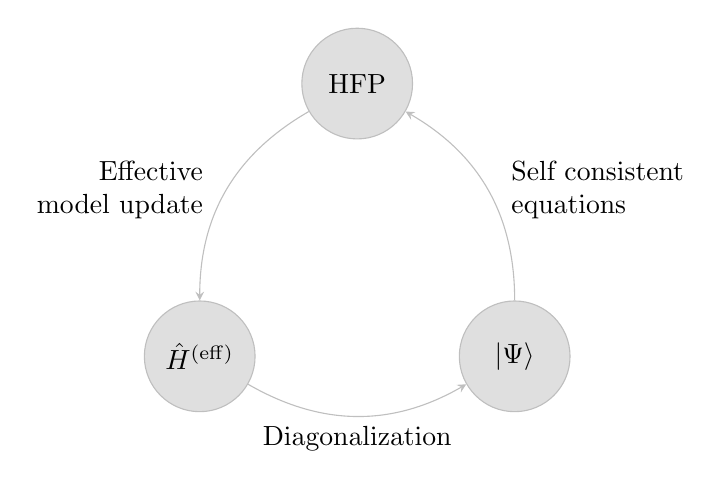
\begin{tikzpicture} 
	
    \node[
        name=he,
        circle,
        draw=lightgray,
        text=black,
        fill=lightgray!50,
        minimum size=4em
    ] 
        (He) at (0,0)
            {$\hat H^{(\mathrm{eff})}$};
            
    \node[
        name=psi,
        circle,
        draw=lightgray,
        text=black,
        fill=lightgray!50,
        minimum size=4em
    ] 
        (PSI) at (4,0)
            {$\ket{\Psi}$};
            
    \node[
        name=hfp,
        circle,
        draw=lightgray,
        text=black,
        fill=lightgray!50,
        align=center,
        minimum size=4em
    ] 
        (HFP) at (2,3.464)
            {HFP};
            
    \draw[color=lightgray, -stealth]
        (He) to[bend right]node[below,color=black]{Diagonalization} (PSI);
    \draw[color=lightgray, -stealth]
        (PSI) to[bend right]node[right,color=black,align=left,xshift=0.5em]{Self consistent\\equations} (HFP);
    \draw[color=lightgray, -stealth]
        (HFP) to[bend right]node[left,color=black,align=right,xshift=-0.5em]{Effective\\model update} (He);

\end{tikzpicture}

	\caption{Schematization of the self-consistent Hartree Fock method described in Sec.~\ref{sec:computational-mft}. The effective model is solved, the solution is used to estimate self-consistently the Hartree Fock vector, which is then used to update iteratively the model itself.}
	\label{fig:effective-model-scheme}
\end{figure}
%
A self consistent Hartree-Fock scheme goes as follows: {\color{tabred}[ Consider adding a point for chemical potential estimation. ]}
\begin{enumerate}
	\item Apply MFT to the quartic hamiltonian, recovering its general theoretic effective form;
	\item Impose selection rules on the parameters $C_{\alpha\beta}$, $D_{\alpha\beta}$, eventually eliminating those not respecting the symmetry sector we are working in\footnote{
		As an example: if we choose not to break charge conservation, set $\forall\alpha,\beta\,\colon\,D_{\alpha\beta}=0$.
	};
	\item Choose a starting value and a coherent symmetry structure for the remaining parameters;
	\item Enter iterative scheme of Fig.~\ref{fig:effective-model-scheme}:
	\begin{enumerate}
		\item Diagonalize the effective hamiltonian $\hat H^{(\mathrm{eff})}[C,D]$ and recover the ground-state $\ket{\Psi [C,D]}$;
		\item Compute the new parameters $C_{\alpha\beta}'$, $D_{\alpha\beta}'$ via the self consistent equations;
		\item Initialize the new effective hamiltonian $\hat H^{(\mathrm{eff})}[C',D']$ and repeat the cycle until convergence.
	\end{enumerate}
\end{enumerate}
Of course, to work any of these algorithms we need to know how to diagonalize the hamiltonian. In the context of the Extended Hubbad Model at thermal equilibrium, due to the phases we are simulating, we know analytically the diagonalized hamiltonian, and making use of this knowledge we are able to reduce the self consistent scheme to a simple iterative algorithm. An explicit example of HF algorithm used in present text, somewhat simplified due to the presence of a single HF parameter, is given in App.~\ref{appsubsec:hartree-fock-algorithm}.

\subsection{Square lattice spatial symmetry structures}

\begin{figure}
	\centering
	\subfloat[Local $s$-wave]{
		\begin{tikzpicture}
	\fill[color=lightgray] 
	(0,0) circle (1.5pt)
		node[anchor=south west, color=black]
			{$1$}
	(1,0) circle (1.5pt)
		node[anchor=west]
			{$0$}
	(-1,0) circle (1.5pt)
		node[anchor=east]
			{$0$}
	(0,1) circle (1.5pt)
		node[anchor=south]
			{$0$}
	(0,-1) circle (1.5pt)
		node[anchor=north]
			{$0$};
			
	\node[anchor=center] 
		at (-1,1)
			{$\varphi^{(s)}_{ij}$};
	
	\draw[color=lightgray, dashed]
		(-1,0) -- (1,0)
		(0,-1) -- (0,1);
\end{tikzpicture}
		\label{subfig:s-wave-correlator}
	}
	\hspace{2em}
	\subfloat[Extended $s$-wave.]{
		\begin{tikzpicture}
	\fill[color=lightgray] 
	(0,0) circle (1.5pt)
	(1,0) circle (1.5pt)
		node[anchor=west, color=black]
			{$g^{(s)}$}
	(-1,0) circle (1.5pt)
		node[anchor=east, color=black]
			{$g^{(s)}$}
	(0,1) circle (1.5pt)
		node[anchor=south, color=black]
			{$g^{(s)}$}
	(0,-1) circle (1.5pt)
		node[anchor=north, color=black]
			{$g^{(s)}$};
	
	\draw[color=lightgray]
	(-1,0) -- (1,0)
	(0,-1) -- (0,1);
\end{tikzpicture}
		\label{subfig:s*-wave-correlator}
	}\\[3em]
	\subfloat[$p_x$-wave.]{
		\begin{tikzpicture}
	\fill[color=lightgray] 
	(0,0) circle (1.5pt)
		node[anchor=south west]
			{$0$}
	(1,0) circle (1.5pt)
		node[anchor=west, color=black]
			{$1$}
	(-1,0) circle (1.5pt)
		node[anchor=east, color=black]
			{$-1$}
	(0,1) circle (1.5pt)
		node[anchor=south]
			{$0$}
	(0,-1) circle (1.5pt)
		node[anchor=north]
			{$0$}
	(0,-1) circle (1.5pt)
		node[anchor=north, opacity=0]
			{$-1$}; % Aligment
			
	\node[anchor=center] 
		at (-1,1)
			{$\varphi^{(p_x)}_{ij}$};
	
	\draw[color=lightgray] 
		(-1,0) -- (1,0);
	\draw[color=lightgray, dashed] 
		(0,-1) -- (0,1);
\end{tikzpicture}
		\label{subfig:px-wave-correlator}
	}
	\hspace{2em}
	\subfloat[$p_y$-wave.]{
		\begin{tikzpicture}
	\fill[color=lightgray] 
	(0,0) circle (1.5pt)
	(1,0) circle (1.5pt)
		node[anchor=west, color=black]
			{$0$}
	(-1,0) circle (1.5pt)
		node[anchor=east, color=black]
			{$0$}
	(0,1) circle (1.5pt)
		node[anchor=south, color=black]
			{$g^{(p_y)}$}
		node[anchor=south, opacity=0] 
			{$g^{(d_{x^2-y^2})}$} 	% Alignment
	(0,-1) circle (1.5pt)
		node[anchor=north, color=black]
			{$-g^{(p_y)}$}
		node[anchor=north, opacity=0] 
			{$g^{(d_{x^2-y^2})}$};	% Alignment;
	
	\draw[color=lightgray, dashed] 
		(-1,0) -- (1,0);
	\draw[color=lightgray] 
		(0,-1) -- (0,1);
\end{tikzpicture}
		\label{subfig:py-wave-correlator}
	}
	\hspace{2em}
	\subfloat[$d_{x^2-y^2}$-wave.]{
		\begin{tikzpicture}
	\fill[color=lightgray] 
	(0,0) circle (1.5pt)
	(1,0) circle (1.5pt)
		node[anchor=west, color=black]
			{$g^{(d_{x^2-y^2})}$}
	(-1,0) circle (1.5pt)
		node[anchor=east, color=black]
			{$g^{(d_{x^2-y^2})}$}
	(0,1) circle (1.5pt)
		node[anchor=south, color=black]
			{$-g^{(d_{x^2-y^2})}$}
	(0,-1) circle (1.5pt)
		node[anchor=north, color=black]
			{$-g^{(d_{x^2-y^2})}$};
	
	\draw[color=lightgray] 
		(-1,0) -- (1,0)
		(0,-1) -- (0,1);
\end{tikzpicture}
		\label{subfig:d-wave-correlator}
	}
	\caption{Form factors at different topologies, as listed in Tab.~\ref{tab:x-wave-real-factors}. In figures five sites are represented: the hub site $i$ and its four NN. Solid lines represent non-zero values for $\varphi_{\bm{\delta}}$, while dashed lines represent vanishing factors.}
	\label{fig:x-wave-real-factors}
\end{figure}

For the $2$D square lattice, various spatial symmetries are possible. Let $i$ be a specific site, and consider a generic function $g_{ij}$ whose domain is given by the site itself and its four NNs (the domain concides with the points of Fig.~\ref{fig:square-nearest-neighbors}). Then it is immediate to see that the function can be written in the following basis
\[
	g_{ij} = \sum_\gamma g^{(\gamma)} \varphi_{ij}^{(\gamma)}
\]
where $g^{(\gamma)}$ are the $g_{ij}$ symmetries-decomposition coefficients while $\varphi_{ij}^{(\gamma)}$ are the form factors listed in Tab.~\ref{tab:x-wave-real-factors}, a simple orthonormal rearrangement of the harmonics basis.

\setlength{\extrarowheight}{0.5em}
\begin{table}
	\centering
	\begin{tabular}{r E l l}
		\textbf{Structure} & \multicolumn{2}{c}{\textbf{Form factor}} & \textbf{Graph} \\
		\midrule
		$s$-wave & $\varphi^{(s)}_{ij}$ & $\delta_{ij}$ & Fig.~\ref{subfig:s-wave-correlator} \\
		Extended $s$-wave & $\varphi^{(s^*)}_{ij}$ &
		$\delta_{j=i+\delta_x} + \delta_{j=i-\delta_x} + \delta_{j=i+\delta_y} + \delta_{j=i-\delta_y}$ & Fig.~\ref{subfig:s*-wave-correlator} \\
		$p_x$-wave & $\varphi^{(p_x)}_{ij}$ & $ 
		\delta_{j=i+\delta_x} - \delta_{j=i-\delta_x}$ & Fig.~\ref{subfig:px-wave-correlator} \\
		$p_y$-wave & $\varphi^{(p_y)}_{ij}$ & $ \delta_{j=i+\delta_y} - \delta_{j=i-\delta_y}$ & Fig.~\ref{subfig:py-wave-correlator} \\
		$d_{x^2-y^2}$-wave & $\varphi^{(d)}_{ij}$ & $
		\delta_{j=i+\delta_x} + \delta_{j=i-\delta_x} - \delta_{j=i+\delta_y} - \delta_{j=i-\delta_y}$ & Fig.~\ref{subfig:d-wave-correlator} \\[0.5em]
		\midrule
	\end{tabular}
	\caption{Form factors for a function defined on a square lattice,- The last column indicates the graph representation of each contribution given in Fig.~\ref{fig:wave-correlators}. Subscript $x^2-y^2$ is omitted for notational clarity.}
	\label{tab:x-wave-real-factors}
\end{table}
\setlength{\extrarowheight}{0em}

Antiferromagnetic ordering considered in this text exhibits a perfect $s \oplus s^*$ topological ordering. Instead, superconductivity is established with a given symmetry -- which means, symmetry breaking in the phase transition proceeds in a specific channel. Conventional $\mathrm{BCS}$ superconductivity arises from the only possible spatial structure of the local pairing, $s$-wave -- here appearing as a local term (Fig.~\ref{subfig:s-wave-correlator}) and extended on a non-local term (Fig.~\ref{subfig:s*-wave-correlator}). Cuprates exhibit a tendency towards $d_{x^2-y^2}$ SC, while other materials towards $p$-wave types -- eventually with some chirality, as is the case for $p_x \pm i p_y$ SCs. To establish SC under a certain symmetry $\gamma$ means that Cooper pairs acquire said symmetry.

\subsection{Symmetry-based optimizations}

When dealing with phases which respect translational symmetry, or at most reduce it to a weaker symmetry by shrinking the Brillouin Zone, it' useful to work in reciprocal space, as discussed in Sec.~\ref{sec:mft-analysis-reciprocal-space}. As said, a particular phase can show specific spatial symmetries, and so will the Hartree Fock parameters. The key point to notice is that self-consistent equations involve sums (or integrals) to be computed over fermionic states, which can be heavily simplified by employing said symmetries. Consider the form factors of Tab.~\ref{tab:x-wave-real-factors}, and their Fourier transforms of Tab.~\ref{tab:x-wave-reciprocal-factors}. If these symmetries are developed by the HFPs, it's of no use to integrate over the entire BZ, since different regions linked by periodicity of the form factors will lead to redundant calculations.

{\color{tabred}[
	Add: plots of the Brillouin zone cut for different symmetries.
]}

\setlength{\extrarowheight}{0.5em}
\begin{table}
	\centering
	\begin{tabular}{r E l l}
		\textbf{Structure} & \multicolumn{2}{c}{\textbf{Structure factor}} & \textbf{Graph} \\
		\midrule
		$s$-wave & $\varphi_\mathbf{k}^{(s)}$ & $1$ & Fig.~\ref{subfig:s-wave-correlator} \\
		Extended $s$-wave & $\varphi^{(s^*)}_{\mathbf{k}}$ & $\cos k_x + \cos k_y$ & Fig.~\ref{subfig:s*-wave-correlator} \\
		$p_x$-wave & $\varphi_\mathbf{k}^{(p_x)}$ & $i \sqrt{2} \sin k_x $ & Fig.~\ref{subfig:px-wave-correlator} \\
		$p_y$-wave & $\varphi_\mathbf{k}^{(p_y)}$ & $i \sqrt{2} \sin k_y$ & Fig.~\ref{subfig:py-wave-correlator} \\
		$d_{x^2-y^2}$-wave & $\varphi_\mathbf{k}^{(d)}$ & $\cos k_x - \cos k_y$ & Fig.~\ref{subfig:d-wave-correlator} \\[0.5em]
		\midrule
	\end{tabular}
	\caption{Structure factors derived from the correlation structures of Tab.~\ref{tab:x-wave-real-factors}. The functions hereby defined are orthonormal.}
	\label{tab:x-wave-reciprocal-factors}
\end{table}
\setlength{\extrarowheight}{0em}

Finally, a very useful detail is given by the following argument. Consider the equation
\[
	\cos \left( \delta k_x \right)	+ \cos \left( \delta k_y \right) = \cos k_x \cos k_x' + \sin k_x \sin k_x' + \cos k_y \cos k_y' + \sin k_y \sin k_y'
\]
For the sake of readability, the notations
\[
	c_\ell \equiv \cos k_\ell
	\qquad
	s_\ell \equiv \sin k_\ell
	\qquad
	c_\ell' \equiv \cos	k_\ell'
	\qquad
	s_\ell' \equiv \sin k_\ell'
\]
are used. Group the four terms above,
\begin{equation}\label{eq:sym-asym-couplings-gap}
	\underbrace{
		\left(c_x c_x' + c_y c_y' \right) 
	}_\text{Symmetric}
	+ \underbrace{
		\left(s_x s_x' + s_y s_y' \right)
	}_\text{Anti-symmetric}
\end{equation}
The first two exhibit inversion symmetry for both arguments $\mathbf{k}$, $\mathbf{k}'$; the second two exhibit anti-symmetry. Decoupling the symmetric part, we obtain
\[
	c_x c_x' + c_y c_y' = \frac{1}{2} (c_x + c_y)(c_x' + c_y') + \frac{1}{2} (c_x - c_y)(c_x' - c_y')
\]
which finally gives:
\[
\begin{aligned}
	\cos \left( \delta k_x \right)	+ \cos \left( \delta k_y  \right) &= \frac{1}{2}  (c_x + c_y)(c_x' + c_y') &&\qquad\text{($s^*$-wave)} \\
	&\hphantom{=}+ s_x s_x' &&\qquad\text{($p_x$-wave)} \\
	&\hphantom{=}+ s_y s_y' &&\qquad\text{($p_y$-wave)} \\
	&\hphantom{=}+ \frac{1}{2} (c_x - c_y)(c_x' - c_y') &&\qquad\text{($d_{x^2-y^2}$-wave)}
\end{aligned}
\]
or, in a more compact form	
\begin{equation}\label{eq:coscos-symmetries-decomposition}
	\cos \left( \delta k_x \right)	+ \cos \left( \delta k_y  \right) = \frac 1 2 \sum_\gamma \varphi_\mathbf{k}^{(\gamma)} \varphi_{\mathbf{k}'}^{(\gamma)*}
	\qq{for $\gamma \in \lbrace s^*, p_x, p_y, d_{x^2-y^2} \rbrace$}
\end{equation}
This decomposition will become particularly handy in later calculations.
\def\GraphicsFolder{parts/mft-analysis/chapters/normal-phase/pictures}
\chapter{The normal phase}\label{chap:normal-phase}

This chapter is devoted to the MFT analysis of the ``normal phase'', which is, the one where interacting electrons do not develop an antiferromagnetic or superconducting gap, although undergoing an effective non-trivial transformation. What will be derived here, in particular the hopping renormalization effect, constitutes a peculiarity of effective MFT treatment of the EHM and will be the groundwork of following analyses. Note that this chapter is structured in such a way that what is derived here mathematically is recovered and expanded to more complex phases in next chapters.

\section{Theoretical description of the ``normal'' phase}

The normal phase is simply the one where no symmetry is broken, and the many-body ground state preserves the entire $\mathrm{U}(2)$ structure of Eq.~\eqref{eq:ehm-global-u2-symmetry-u1-su2} as well as translational symmetry. Thus, the normal phase is essentially given by the null gap limit of both the antiferromagnetic and superconducting phases. By discussing it separately now, we highlight a MFT feature of the EHM of particular interest. From Tabs.~\ref{tab:U-wick-terms-phases} and \ref{tab:V-wick-terms-phases}, we know that the relevant Wick's contractions (RWCs) for this phase are
\[
\begin{aligned}
	&\hat H_U 
	&&\text{Hartree contraction} \\
	&\hat H_V \text{ (o.s. sector)}
	&&\text{Hartree contraction} \\
	&\hat H_V \text{ (s.s. sector)}
	&&\text{Hartree and Fock contractions} \\
\end{aligned}	
\]
and since the phase we are establishing obeys translational symmetry, we also know Hartree terms are essentially chemical potential shifts. Next section derives this effect in detail.

\subsection{Hartree shift of $\mu$}\label{subsec:hartree-shifts-mu}

In the context of numerical simulations at fixed density, the chemical potential is determined self-consistently; thus any net effect that shifts $\mu$ is effectively ignored within the iterative algorithm. For the sake of completeness, we hereby derive the effect analytically.

\paragraph{Local repulsion.}

In the normal phase, the local repulsion $\hat H_U$ only contributes through Hartree-like RWCs,
\[
	\hat H_U \simeq
	U \sum_{i} \left[
		\langle 
			\hat n_{i\uparrow}
		\rangle \hat n_{i\downarrow} + \hat n_{i\uparrow} \langle 
			\hat n_{i\downarrow}
		\rangle - \langle 
			\hat n_{i\downarrow}
		\rangle \langle 
			\hat n_{i\uparrow}
			\rangle
	\right]
\]
For a translationally invariant phase such as the normal phase, it holds
\begin{equation}\label{eq:normal-density-ansatz}
	\langle \hat n_{i\sigma} \rangle = n
\end{equation}
which gives immediately
\[
\begin{aligned}
	\hat H_U &\simeq
	nU \sum_i \left[
		 \hat n_{i\uparrow} + \hat n_{i\downarrow}
	\right]
	- U \sum_i n^2 \\
	&= nU \times \hat N - E_{\mathrm{H}/U}^{(\mathrm{N})}
\end{aligned}
\]
being $\hat N$ the total number operator and $ E_{\mathrm{H}/U}^{(\mathrm{N})}$ the ``contraction energy'' (also known as double counting term) due to the Hartree (H) contraction of the $U$ repulsion,
\[
	 E_{\mathrm{H}/U}^{(\mathrm{N})} = nU \times L_x L_y
\]
which correctly is a linearly extensive quantity. The chemical potential is corrected by
\begin{equation}\label{eq:local-hartree-mu-shift}
	\mu \to \mu - nU
\end{equation}
The non-local attraction further corrects $\mu$.

\paragraph{Non-local attraction.}

Let us break down $\hat H_V$ isolating its Hartree RWCs in both o.s. and s.s. sectors:
\begin{multline*}
	\hat H_V \simeq 
	\overbrace{
		-V \sum_{\ev{ij}} \sum_\sigma \left[
			\langle 
			\hat n_{i\sigma}
			\rangle \hat n_{j\sigma} + \hat n_{i\sigma} \langle 
			\hat n_{j\sigma}
			\rangle - \langle 
			\hat n_{i\sigma}
			\rangle \langle 
			\hat n_{j\sigma}
			\rangle
		\right]
	}^{\mathrm{s.s.}} \\
	\underbrace{
		-V \sum_{\ev{ij}} \sum_\sigma \left[
			\langle
			\hat n_{i\sigma}
			\rangle \hat n_{j\overline{\sigma}} + \hat n_{i\sigma} \langle 
			\hat n_{j\overline{\sigma}}
			\rangle
			- \langle 
			\hat n_{i\sigma}
			\rangle \langle 
			\hat n_{j\overline{\sigma}}
			\rangle
		\right]
	}_{\mathrm{o.s.}} \, +\, 
	(\text{all the rest})
\end{multline*}
where ``all the rest'' collects all non-Hartree RWCs. Recalling the Ansatz of Eq.~\eqref{eq:normal-density-ansatz}, we get
\[
	\hat H_V \simeq  \underbrace{
		-nV \sum_{\ev{ij}} \sum_\sigma \left[
		\hat n_{j\sigma} + \hat n_{i\sigma}
		\right]
	}_{\mathrm{s.s.}}
	\underbrace{
		-nV \sum_{\ev{ij}} \sum_\sigma \left[
		\hat n_{j\overline{\sigma}} + \hat n_{i\sigma}
		\right]
	}_{\mathrm{o.s.}} 
	- E_{\mathrm{H}/V}^{(\mathrm{N})}
	+ (\text{all the rest})
\]
with $E_{\mathrm{H}/V}^{(\mathrm{N})}$ the normal state shift to energy brought by $\hat H_V$,
\[
	E_{\mathrm{H}/V}^{(\mathrm{N})} = 2V \sum_{\ev{ij}} \sum_\sigma n^2 = 4n^2 V \times \frac{z}{2} L_x L_y
\]
being $z=4$ the coordination number for the $2$D square lattice. Now, evidently both sums above are just a number operator,
\[
	\hat H_V \simeq -2nzV \times \hat N + 
	(\text{all the rest})
\]
This accounts for the final Hartree shift of $\mu$,
\begin{equation}\label{eq:non-local-hartree-mu-shift}
	\mu \to \mu + 2znV
\end{equation}
Thus, when considering the net shift to $\mu$ due to both interactions, we get
\begin{equation}\label{eq:total-hartree-mu-shift}
	\tilde{\mu} \equiv \mu + n(2zV-U)
\end{equation}
This result remains valid in all phases discussed in this text: for the AF phase, the SDW character leaves this shift untouched, while the superconducting phase we are discussion is inherently translational invariant.

\subsection{Fock hopping renormalization in the normal phase}\label{subsec:fock-hopping-renormalization-normal}

The most relevant effect brought by the presence of $\hat H_V$ is hopping renormalization. From Wick's decomposition of $\hat H_V$, the only allowed Fock term comes from the same-spin part due to $\mathrm{SU}(2)$ symmetry selection rules. Let us focus only on this term when decomposing $\hat H$:
\begin{equation}\label{eq:real-space-non-local-interaction-fock}
	\hat H_V \simeq 
	V \sum_{\ev{ij}} \sum_\sigma \left[
		\langle
		\hat c_{i\sigma}^\dagger \hat c_{j\sigma}
		\rangle \hat c_{j\sigma}^\dagger  \hat c_{i\sigma} + 
		\hat c_{i\sigma}^\dagger \hat c_{j\sigma}
		\langle \hat c_{j\sigma}^\dagger  \hat c_{i\sigma} \rangle - \langle \hat c_{i\sigma}^\dagger \hat c_{j\sigma}
		\rangle \langle \hat c_{j\sigma}^\dagger  \hat c_{i\sigma} \rangle
	\right] + (\text{all the rest})
\end{equation}
(note the $+$ sign in front of the displayed term). A bond-wise hopping amplitude can be defined,
\[
	\tilde{t}_{ij\sigma} \equiv t - V \langle
	\hat c_{j\sigma}^\dagger \hat c_{i\sigma}
	\rangle
\]
In all phases considered in the present discussion, given some site $i$ and a spin $\sigma$, evidently $\tilde{t}_{ij\sigma}$ must be identical for any NN site $j$. Over the planar square lattice, this implies that the quantity $\langle
\hat c_{j\sigma}^\dagger \hat c_{i\sigma} \rangle$ exhibits $s^*$-wave symmetry (also referred to as ``Extended $s$-wave symmetry'') given in Tab.~\ref{tab:x-wave-real-factors} and depicted in Fig.~\ref{subfig:s*-wave-correlator}. This gives in turn that the hopping shift is rigid and the bands are rigidly renormalized by a self consistent parameter $w^{(\mathrm{N})}$,
\[
	t\to\tilde{t} \equiv t - w^{(\mathrm{N})}V
	\quad\implies\quad
	\epsilon_\mathbf{k} \to \tilde{\epsilon}_\mathbf{k} = -2 \tilde{t} \left(
		\cos k_x + \cos k_y
	\right)
\]

The effective diffusive hamiltonian is given by
\[
\begin{aligned}
	\hat H_{\tilde{t}} &= \hat H_t + V \sum_{\ev{ij}} \sum_\sigma \left[
	\langle
	\hat c_{i\sigma}^\dagger \hat c_{j\sigma}
	\rangle \hat c_{j\sigma}^\dagger  \hat c_{i\sigma} + \hc
	\right] \\
	&= - \sum_{\ev{ij}} \sum_\sigma 
	\left[
	\tilde{t}_{ij\sigma} \hat c_{i\sigma}^\dagger \hat c_{j\sigma} + \hc
	\right]
\end{aligned}
\]
In reciprocal space, the effective hopping must be transformed as well. Consider the Fourier Transform $\mathcal{F}$ given in Eq.~\eqref{eq:reciprocal-space-non-local-interaction-explicit}, applied to the displayed part of Eq.~\eqref{eq:real-space-non-local-interaction-fock},
\begin{multline}
	V \sum_{\ev{ij}} \sum_\sigma \left[
		\langle
		\hat c_{i\sigma}^\dagger \hat c_{j\sigma}
		\rangle \hat c_{j\sigma}^\dagger  \hat c_{i\sigma} + 
		\hat c_{i\sigma}^\dagger \hat c_{j\sigma}
		\langle \hat c_{j\sigma}^\dagger  \hat c_{i\sigma} \rangle - \langle \hat c_{i\sigma}^\dagger \hat c_{j\sigma}
		\rangle \langle \hat c_{j\sigma}^\dagger  \hat c_{i\sigma} \rangle
	\right] \\
	\stackrel{\mathcal{F}}{=} \frac{2V}{L_x L_y} \sum_{\mathbf{K}, \mathbf{k}, \mathbf{k}'} \sum_\sigma \left[
	\cos \left(
	\delta k_x
	\right)	+ \cos \left(
	\delta k_y
	\right)	
	\right]	
	\langle
	\hat c_{\mathbf{K}+\mathbf{k} \sigma}^\dagger 
	\hat c_{\mathbf{K}-\mathbf{k}' \sigma}
	\rangle
	\hat c_{\mathbf{K}-\mathbf{k} \sigma}^\dagger  \hat c_{\mathbf{K}+\mathbf{k}'\sigma} - E_{\mathrm{F}/V}^{(\mathrm{N})} \label{eq:normal-V-fock-int1}
\end{multline}
Here, the $2$ prefactor comes from recognizing that the first two operators in square brackets in the first line generate identical contributions to the full sum; the double counting energy shift is given by
\begin{equation}\label{eq:reciprocal-space-non-local-interaction-fock-double-couting}
	E_{\mathrm{F}/V}^{(\mathrm{N})} \equiv \frac{V}{L_x L_y} \sum_{\mathbf{K}, \mathbf{k}, \mathbf{k}'} \sum_\sigma \left[
		\cos \left(
			\delta k_x
		\right)	+ \cos \left(
			\delta k_y
		\right)	
	\right]	
	\langle
		\hat c_{\mathbf{K}+\mathbf{k} \sigma}^\dagger 
	\hat c_{\mathbf{K}-\mathbf{k}' \sigma}
	\rangle \langle
		\hat c_{\mathbf{K}-\mathbf{k} \sigma}^\dagger  \hat c_{\mathbf{K}+\mathbf{k}'\sigma} 
	\rangle
\end{equation}

Up to this point, this derivation is general and will be re-used in next chapters. Here the specificity of the physical phase settles in: if we assume the normal state to be a free degenerate Fermi gas with renormalized bands, we get
\[
	\langle \hat c_{\mathbf{k}_1\sigma_1} \hat c_{\mathbf{k}_2 \sigma_2} \rangle = \delta_{\mathbf{k}_1=\mathbf{k}_2} \delta_{\sigma_1=\sigma_2} f(\tilde{\epsilon}_\mathbf{k};\beta,\tilde{\mu})
\]
being $f$ the Fermi-Dirac distribution,
\[
	f(\epsilon;\beta,\mu) \equiv \frac{1}{e^{\beta(\epsilon-\mu)}+1}
\]
It follows that Eq.~\eqref{eq:normal-V-fock-int1} becomes
\begin{multline}
	V \sum_{\ev{ij}} \sum_\sigma \left[
	\langle
	\hat c_{i\sigma}^\dagger \hat c_{j\sigma}
	\rangle \hat c_{j\sigma}^\dagger  \hat c_{i\sigma} + 
	\hat c_{i\sigma}^\dagger \hat c_{j\sigma}
	\langle \hat c_{j\sigma}^\dagger  \hat c_{i\sigma} \rangle - \langle \hat c_{i\sigma}^\dagger \hat c_{j\sigma}
	\rangle \langle \hat c_{j\sigma}^\dagger  \hat c_{i\sigma} \rangle
	\right] \\
	\stackrel{\mathcal{F}}{=} \frac{2V}{L_x L_y} \sum_{\mathbf{K}, \mathbf{k}} \sum_\sigma \left[
	\cos \left(
	2 k_x
	\right)	+ \cos \left(
	2 k_y
	\right)	
	\right]	
	\langle
	\hat c_{\mathbf{K}+\mathbf{k} \sigma}^\dagger 
	\hat c_{\mathbf{K}+\mathbf{k} \sigma}
	\rangle
	\hat c_{\mathbf{K}-\mathbf{k} \sigma}^\dagger  \hat c_{\mathbf{K}-\mathbf{k}\sigma} - E_{\mathrm{F}/V}^{(\mathrm{N})} \label{eq:normal-V-fock-int2}
\end{multline}
since the only contribution comes from $\mathbf{k}'=-\mathbf{k}$. Let now $\mathbf{q}\equiv\mathbf{K}+\mathbf{k}$, $\mathbf{q}'\equiv\mathbf{K}-\mathbf{k}$. Being for $\ell=x,y$
\[
\begin{aligned}
	\delta q_\ell &\equiv q_\ell - q_\ell' \\
	&= (K_\ell+k_\ell) - (K_\ell-k_\ell) \\
	&= 2k_\ell
\end{aligned}
\]
we reduce Eq.~\eqref{eq:normal-V-fock-int1} to
\begin{multline}
	V \sum_{\ev{ij}} \sum_\sigma \left[
	\langle
	\hat c_{i\sigma}^\dagger \hat c_{j\sigma}
	\rangle \hat c_{j\sigma}^\dagger  \hat c_{i\sigma} + 
	\hat c_{i\sigma}^\dagger \hat c_{j\sigma}
	\langle \hat c_{j\sigma}^\dagger  \hat c_{i\sigma} \rangle - \langle \hat c_{i\sigma}^\dagger \hat c_{j\sigma}
	\rangle \langle \hat c_{j\sigma}^\dagger  \hat c_{i\sigma} \rangle
	\right] \\
	\stackrel{\mathcal{F}}{=} \frac{2V}{L_x L_y} \sum_{\mathbf{q}, \mathbf{q}'} \sum_\sigma \left[
		\cos \left(
			\delta q_x
		\right)	+ \cos \left(
			\delta q_y
		\right)	
	\right]	
	\langle
		\hat c_{\mathbf{q}\sigma}^\dagger 
		\hat c_{\mathbf{q}\sigma}
	\rangle
	\hat c_{\mathbf{q}'\sigma}^\dagger  \hat c_{\mathbf{q}'\sigma} - E_{\mathrm{F}/V}^{(\mathrm{N})} \label{eq:normal-V-fock-int3}
\end{multline}
Recall now the result of Eq.~\eqref{eq:coscos-symmetries-decomposition},
\[
	\cos \left( \delta q_x \right)	+ \cos \left( \delta q_y  \right) = \frac 1 2 \sum_\gamma \varphi_\mathbf{q}^{(\gamma)} \varphi_{\mathbf{q}'}^{(\gamma)*}
	\qq{for $\gamma \in \lbrace s^*, p_x, p_y, d_{x^2-y^2} \rbrace$}
\]
Thanks to this handy property, we reduce Eq.~\eqref{eq:normal-V-fock-int3} to
\begin{multline}
	V \sum_{\ev{ij}} \sum_\sigma \left[
	\langle
	\hat c_{i\sigma}^\dagger \hat c_{j\sigma}
	\rangle \hat c_{j\sigma}^\dagger  \hat c_{i\sigma} + 
	\hat c_{i\sigma}^\dagger \hat c_{j\sigma}
	\langle \hat c_{j\sigma}^\dagger  \hat c_{i\sigma} \rangle - \langle \hat c_{i\sigma}^\dagger \hat c_{j\sigma}
	\rangle \langle \hat c_{j\sigma}^\dagger  \hat c_{i\sigma} \rangle
	\right] \\
	\stackrel{\mathcal{F}}{=} \sum_\gamma \left[
		\frac{1}{L_x L_y} \sum_\mathbf{q} \varphi_\mathbf{q}^{(\gamma)}
		\langle
			\hat c_{\mathbf{q}\sigma}^\dagger 
			\hat c_{\mathbf{q}\sigma}
		\rangle
	\right] \times V
	\sum_{\mathbf{q}'}
	\varphi_{\mathbf{q}'}^{(\gamma)*}
	\hat c_{\mathbf{q}'\sigma}^\dagger
	\hat c_{\mathbf{q}'\sigma} - E_{\mathrm{F}/V}^{(\mathrm{N})} \label{eq:normal-V-fock-int4}
\end{multline}
Now, the bare bands $\epsilon_\mathbf{k}$ as well as their rigidly renormalized version $\tilde{\epsilon}_\mathbf{k}$ are $s^*$-wave symmetric. The expectation value $\langle \hat c_{\mathbf{q}\sigma}^\dagger \hat c_{\mathbf{q}\sigma} \rangle = f(\tilde{\epsilon}_\mathbf{q};\beta,\tilde{\mu})$ thus exhibits the same symmetry. Then, in Eq.~\eqref{eq:normal-V-fock-int4}, due to the presence of the part in square brackets, only $\gamma=s^*$ contributes. Let us define the HFP $w^{(\mathrm{N})}$ as
\begin{equation}\label{eq:w-normal-sc-equation}
	w^{(\mathrm{N})} \equiv \frac{1}{2L_x L_y} \sum_{\mathbf{q}\in\mathrm{BZ}} \left(
		\cos q_x + \cos q_y
	\right) f(\tilde{\epsilon}_\mathbf{q};\beta,\tilde{\mu})
\end{equation}
which finally gives
\begin{multline}
	V \sum_{\ev{ij}} \sum_\sigma \left[
	\langle
	\hat c_{i\sigma}^\dagger \hat c_{j\sigma}
	\rangle \hat c_{j\sigma}^\dagger  \hat c_{i\sigma} + 
	\hat c_{i\sigma}^\dagger \hat c_{j\sigma}
	\langle \hat c_{j\sigma}^\dagger  \hat c_{i\sigma} \rangle - \langle \hat c_{i\sigma}^\dagger \hat c_{j\sigma}
	\rangle \langle \hat c_{j\sigma}^\dagger  \hat c_{i\sigma} \rangle
	\right] \\
	\stackrel{\mathcal{F}}{=} 
	\sum_{\mathbf{q}'}
	2 w^{(\mathrm{N})} V
	\left(
		\cos q_x + \cos q_y
	\right)
	\hat c_{\mathbf{q}'\sigma}^\dagger
	\hat c_{\mathbf{q}'\sigma} - E_{\mathrm{F}/V}^{(\mathrm{N})} \label{eq:normal-V-fock}
\end{multline}
As anticipated, hopping gets shifted by an amount
\begin{equation}\label{eq:normal-V-fock-t-shift}
	t\to\tilde{t} \equiv t - w^{(\mathrm{N})}V
\end{equation}
with $w^{(\mathrm{N})}$ to be self-consistently determined by iteratively solving Eq.~\eqref{eq:w-normal-sc-equation}.

\begin{table}
	\centering
	\begin{tabular}{c c c c}
		\textbf{Operator} & \textbf{Sector} & \textbf{RWCs} & \textbf{Net effect} \\
		\midrule
		$\hat H_U$ && Hartree & $\mu$ shift \\
		$\hat H_V$ & o.s. & Hartree & $\mu$ shift \\
		\multirow{2}{*}{$\hat H_V$} & \multirow{2}{*}{s.s.} & Hartree & $\mu$ shift\\
		&& Fock & $t$ shift\\
		\midrule
	\end{tabular}
	\caption{}
	\label{}
\end{table}

\section{Free energy density}
\todo

\section{HF results}
\todo
%\def\GraphicsFolder{parts/mft-analysis/chapters/antiferromagnetic-instability/pictures}
\chapter{Anti-Ferromagnetic instability}\label{chap:mft-af-instability}

This chapter is devoted to an in-depth discussion of the antiferromagnetic (AF) long-range ordering in the EHM by the means of MFT. In the context of the $2$D Hubbard model (HM), discussed in App.~\ref{appendix:mean-field-hubbard}, AF ordering establishes as an unconventional metallic phase which is only stable at half-filling (as is discussed in Sec.~\mref). The situation for the EHM is similar: the present analysis is carried out based on the argument that, given the symmetry structure of the non-local NN interaction, the fundamental features of the commensurate AF phase of the HM are effectively preserved, while the parameters are redefined by the interaction itself. The two most relevant effects we discuss in this chapter are the ``magnetization boost'' (Sec.~\mref) and the ``hopping renormalization`` (Sec.~\mref), the latter being a general feature of the EHM common to all phases preserving (or, at most, weakening without destroying) the translational invariance, discussed in Sec.~\ref{subsec:fock-hopping-renormalization-normal}.

\section{Sketch and general features of the MFT solution}
\todo
\subsection{Symmetry considerations for the AF phase}
\todo
\subsection{Antiferromagnetism in the conventional Hubbard model}

Within the Hubbard model, the antiferromagnetic phase (AF) is specified by the Ansatz \eqref{appeq:af-mean-field-ansatz} which is explicitly breaking translational invariance in each spin sector, while preserving $\mathrm{U}^z(1)$ and $\mathrm{U}^c(1)$ symmetries and reduces the hamiltonian to the form of Eq.~\eqref{appeq:hubbard-mean-field-hamiltonian} (ignoring the double-counting terms)
\[
	\hat H_t + \hat H_U \stackrel{\mathrm{MFT}}{\simeq} -t \sum_{\langle \mathbf{r}\mathbf{r}' \rangle} \sum_\sigma \hat c_{\mathbf{r}\sigma}^\dagger \hat c_{\mathbf{r}'\sigma}
	+ nU \sum_\mathbf{r} \left[
		\hat n_{\mathbf{r}\uparrow} + \hat n_{\mathbf{r}\downarrow}
	\right] - mU \sum_\mathbf{r} (-1)^{x+y} \left[
		\hat n_{\mathbf{r}\uparrow} - \hat n_{\mathbf{r}\downarrow}
	\right]
\]
In reciprocal space, the hamiltonian decomposes as in Eq.~\eqref{appeq:hubbard-bogoliubov-hamiltonian},
\[
	\hat H_t + \hat H_U \stackrel{\mathrm{MFT}}{\simeq} \sum_{\mathbf{k} \in \mathrm{MBZ}} \sum_\sigma \hat \Psi_{\mathbf{k}\sigma}^\dagger h_{\mathbf{k}\sigma} \hat \Psi_{\mathbf{k}\sigma}
	\qq{being}
	h_{\mathbf{k}\sigma} \equiv \begin{bmatrix}
		\epsilon_\mathbf{k} & -\Delta_\sigma \\
		-\Delta_\sigma & - \epsilon_\mathbf{k}
	\end{bmatrix}
\]
and $\Delta_\uparrow = mU$, $\Delta_\downarrow = -mU$. Nambu spinorial formulation is used,
\[
\hat \Psi_{\mathbf{k}\sigma} \equiv \begin{bmatrix}
	\hat c_{\mathbf{k}\sigma} \\
	\hat c_{\mathbf{k}+\bm{\pi}\sigma} 
\end{bmatrix}
\]
and the free electrons energy is simply the tight binding energy
\[
	\epsilon_\mathbf{k} = -2t \left(
		\cos k_x + \cos k_y
	\right)
\]
which is spin-invariant. The MFT description of the model reduces to a gas of free ``$\gamma$-fermions'', described by the Nambu spinor of Eq.~\eqref{appeq:af-diagonalized-nambu-spinor},
\[
	\hat\Gamma_{\mathbf{k}\sigma} = W_{\mathbf{k}\sigma} \hat \Psi_{\mathbf{k}\sigma} = \begin{bmatrix}
		\hat \gamma_{\mathbf{k}\sigma}^{(-)} \\ \hat \gamma_{\mathbf{k}\sigma}^{(+)}
	\end{bmatrix}
\]
where
\[
	W_{\mathbf{k}\sigma} = \begin{bmatrix}
		- \sin \theta_{\mathbf{k}\sigma} & - \cos \theta_{\mathbf{k}\sigma} \\ 
		\cos \theta_{\mathbf{k}\sigma} & - \sin \theta_{\mathbf{k}\sigma}
	\end{bmatrix}
	\qq{and}
	\sin 2\theta_{\mathbf{k}\sigma} \equiv \frac{\Delta_\sigma}{E_\mathbf{k}}
\]
These fermions populate the two bands $\pm E_\mathbf{k} = \sqrt{\epsilon_\mathbf{k}^2 + \Delta^2}$. The entire system is mapped onto an ensemble of pseudo-spins, each subject to a pseudo-field, as in Fig.~\ref{fig:pseudo-magnetic-field}. To diagonalize the system essentially means to align each pseudo-spin with the $z$ axis. Within on the notation of Fig.~\ref{appfig:pseudo-magnetic-field}, the following expectations values hold:
\begin{align}
	\langle \hat \Psi_{\mathbf{k}\sigma}^\dagger \tau^x \hat \Psi_{\mathbf{k}\sigma} \rangle &= \sin \normalfont(2\theta_\mathbf{k})  \langle \hat \Gamma_{\mathbf{k}\sigma}^\dagger \tau^z \hat \Gamma_{\mathbf{k}\sigma} \rangle \label{eq:af-x-expectation}\\
	\langle \hat \Psi_{\mathbf{k}\sigma}^\dagger \tau^y \hat \Psi_{\mathbf{k}\sigma} \rangle &= 0\\
	\langle \hat \Psi_{\mathbf{k}\sigma}^\dagger \tau^z \hat \Psi_{\mathbf{k}\sigma} \rangle &= -\cos \normalfont(2\theta_\mathbf{k}) \langle \hat \Gamma_{\mathbf{k}\sigma}^\dagger \tau^z \hat \Gamma_{\mathbf{k}\sigma} \rangle \label{eq:af-z-expectation}
\end{align}
and since the $\gamma$-fermions are free and in the rotated frame the pseudo-field points ``up'',
\begin{equation}\label{eq:af-rot-z-expectation}
	\langle \hat \Gamma_{\mathbf{k}\sigma}^\dagger \tau^z \hat \Gamma_{\mathbf{k}\sigma} \rangle = \frac{1}{2} \left[
		f\left(
			-E_\mathbf{k};\beta,\mu
		\right) - f\left(
			E_\mathbf{k};\beta,\mu
		\right)
	\right]
\end{equation}
Of these properties, to pseudospin picture is a simple and powerful tool that our MFT discussion should preserve.

\subsection{Extension to the EHM}

Consider now the non-local interaction $\hat H_V$: since only translational invariance is partially broken in the AF phase, the only relevant contributions coming from Wick's decomposition are Hartree terms and the same-spin Fock term. The discussion is thus essentially the same as for the normal phase of Chap.~\ref{chap:normal-phase}, with the only relevant difference being the Ansatz we use in Eq.~\eqref{eq:normal-density-ansatz}, substituted by the commensurate oscillatory Ansatz of Eq.~\eqref{appeq:af-mean-field-ansatz}. As for the normal phase, by design the MFT solution to the model for the given phase is described by a redefinition of the various physical quantities and mathematical objects,
\[
	t \to \tilde{t}
	\qquad
	\epsilon_\mathbf{k} \to \tilde{\epsilon}_{\mathbf{k}\sigma}
	\qquad
	E_\mathbf{k} \to \tilde{E}_{\mathbf{k}\sigma}
	\qquad
	\Delta_\sigma \to \tilde{\Delta}_{\mathbf{k}\sigma}
	\qquad
	\mu \to \tilde{\mu}
\]
The band energies renormalization is simply
\[
	\tilde{E}_{\mathbf{k}\sigma} \equiv \sqrt{\tilde{\epsilon}_{\mathbf{k}\sigma}^2 + |\tilde{\Delta}_{\mathbf{k}\sigma}|^2}
\]
and the following relations hold (the \textit{tilde} sign indicates the renormalized quantity):
\begin{align}
	\langle \hat \Psi_{\mathbf{k}\sigma}^\dagger \tau^x \hat \Psi_{\mathbf{k}\sigma} \rangle &= \sin \normalfont(2\tilde{\theta}_\mathbf{k}) \sin \normalfont(2\tilde{\zeta}_\mathbf{k}) \langle \hat \Gamma_{\mathbf{k}\sigma}^\dagger \tau^z \hat \Gamma_{\mathbf{k}\sigma} \rangle \label{eq:af-x-expectation-non-local}\\
	\langle \hat \Psi_{\mathbf{k}\sigma}^\dagger \tau^y \hat \Psi_{\mathbf{k}\sigma} \rangle &= \sin \normalfont(2\tilde{\theta}_\mathbf{k}) \cos \normalfont(2\tilde{\zeta}_\mathbf{k}) \langle \hat \Gamma_{\mathbf{k}\sigma}^\dagger \tau^z \hat \Gamma_{\mathbf{k}\sigma} \rangle \label{eq:af-y-expectation-non-local}\\
	\langle \hat \Psi_{\mathbf{k}\sigma}^\dagger \tau^z \hat \Psi_{\mathbf{k}\sigma} \rangle &= -\cos \normalfont(2\tilde{\theta}_\mathbf{k}) \langle \hat \Gamma_{\mathbf{k}\sigma}^\dagger \tau^z \hat \Gamma_{\mathbf{k}\sigma} \rangle \label{eq:af-z-expectation-non-local}
\end{align}
with:
\begin{equation}\label{eq:af-bogoliubov-angle-relations}
	\sin \normalfont(2\tilde{\xi}_\mathbf{k}) = \frac{\Re\{\tilde{\Delta}_\mathbf{k}\}}{|\tilde{\Delta}_\mathbf{k}|}
	\qquad
	\cos \normalfont(2\tilde{\xi}_\mathbf{k}) = \frac{\Im\{\tilde{\Delta}_\mathbf{k}\}}{|\tilde{\Delta}_\mathbf{k}|}
	\qquad
	\sin \normalfont(2\tilde{\theta}_\mathbf{k}) = \frac{|\tilde{\Delta}_\mathbf{k}|}{\tilde{E}_\mathbf{k}}
	\qquad
	\cos \normalfont(2\tilde{\theta}_\mathbf{k}) = \frac{\tilde{\epsilon}_\mathbf{k}}{\tilde{E}_\mathbf{k}}
\end{equation}
The physical behavior is the same as for the pure Hubbard model. In terms of MFT discussion, the AF phase is similar enough to the normal phase of Chap.~\ref{chap:normal-phase}: the RWCs are the same of Sec.~\ref{sec:normal-phase-introduction}, listed in Tabs.~\ref{tab:U-wick-terms-phases} and \ref{tab:V-wick-terms-phases}. All three Hartree contractions, responsible in the normal phase of the chemical potential shift, and the s.s. Fock contraction, that originated the hopping renormalization. Let us start by the Hartree terms: due to the ``staggered'' nature of the commensurate AF phase, their role is here more complex. Then we will move to the Fock term, discussing the MFT approximations effect on bands. Next sections are basically an extension of the calculations of Chap.~\ref{chap:normal-phase}.

\begin{figure}
	\centering
	\def\reDeltaParameter{0.8}
\def\imDeltaParameter{0.55}
\def\EpsilonParameter{0.3}
\def\r{1.5}
\pgfmathsetmacro{\DeltaParameter}{sqrt(\reDeltaParameter2 + \imDeltaParameter^2)}
\pgfmathsetmacro{\XiParameter}{atan(\imDeltaParameter/\reDeltaParameter)}

\begin{tikzpicture}
	\begin{axis}[
			axis lines=center,
			axis on top,
			%
			xlabel={$x$},
			ylabel={$y$},
			zlabel={$z$},
			xlabel style={below right},
			ylabel style={right},
			zlabel style={above},
			%
			xtick={-\reDeltaParameter},
			xticklabel={$-\Re\{\tilde{\Delta}_\mathbf{k}\}$},
			xticklabel style={above right},
			extra x ticks={\reDeltaParameter},
			extra x tick labels={$\Re\{\tilde{\Delta}_\mathbf{k}\}$},
			extra x tick style={xticklabel style={below left,yshift=-0.25em}},		
			%
			ytick={-\imDeltaParameter},
			yticklabel={$-\Im\{\tilde{\Delta}_\mathbf{k}\}$},
			yticklabel style={below,yshift=-0.25em},
			extra y ticks={\imDeltaParameter},
			extra y tick labels={$\Im\{\tilde{\Delta}_\mathbf{k}\}$},
			extra y tick style={yticklabel style={above,yshift=0.25em}},	
			%
			ztick={-\EpsilonParameter},
			extra z ticks={\EpsilonParameter},
			zticklabels={$-\tilde{\epsilon}_\mathbf{k}$,$\tilde{\epsilon}_\mathbf{k}$},
			zticklabel style={left},
			extra z ticks={\EpsilonParameter},
			extra z tick labels={$\tilde{\epsilon}_\mathbf{k}$},
			extra z tick style={zticklabel style={right,xshift=0.2em}},
			%
			xmin=-1, xmax=1,
			ymin=-1, ymax=1,
			zmin=-0.6, zmax=0.6,
			view/h=62,
			view/v=30,
			scale=2.25,
		]
		
		% Dashed lines
%		\draw[color=lightgray,dashed]
%			(axis cs:-\reDeltaParameter,0,0) -- (axis cs:-\reDeltaParameter,0,\EpsilonParameter);
%		\draw[color=lightgray,dashed]
%			(axis cs:0,0,\EpsilonParameter) -- (axis cs:-\reDeltaParameter,0,\EpsilonParameter);
%		\draw[color=lightgray,dashed]
%			(axis cs:\reDeltaParameter,0,0) -- (axis cs:\reDeltaParameter,0,-\EpsilonParameter);
%		\draw[color=lightgray,dashed]
%			(axis cs:0,0,-\EpsilonParameter) -- (axis cs:\reDeltaParameter,0,-\EpsilonParameter);

		\draw[color=lightgray,dashed]
			(axis cs:-\reDeltaParameter,-\imDeltaParameter,0) -- (axis cs:-\reDeltaParameter,-\imDeltaParameter,\EpsilonParameter);
		\draw[color=lightgray,dashed]
			(axis cs:0,0,\EpsilonParameter) -- (axis cs:-\reDeltaParameter,-\imDeltaParameter,\EpsilonParameter);
		\draw[color=lightgray,dashed]
			(axis cs:-\reDeltaParameter,-\imDeltaParameter,0) -- (axis cs:\reDeltaParameter,\imDeltaParameter,0);
		\draw[color=lightgray,dashed]
			(axis cs:\reDeltaParameter,\imDeltaParameter,0) -- (axis cs:\reDeltaParameter,\imDeltaParameter,-\EpsilonParameter);
		\draw[color=lightgray,dashed]
			(axis cs:0,0,-\EpsilonParameter) -- (axis cs:\reDeltaParameter,\imDeltaParameter,-\EpsilonParameter);
		\draw[color=lightgray,dashed]
			(axis cs:-\reDeltaParameter,-\imDeltaParameter,0) -- (axis cs:-\reDeltaParameter,0,0);
		\draw[color=lightgray,dashed]
			(axis cs:-\reDeltaParameter,-\imDeltaParameter,0) -- (axis cs:0,-\imDeltaParameter,0);
		\draw[color=lightgray,dashed]
			(axis cs:\reDeltaParameter,\imDeltaParameter,0) -- (axis cs:\reDeltaParameter,0,0);
		\draw[color=lightgray,dashed]
			(axis cs:\reDeltaParameter,\imDeltaParameter,0) -- (axis cs:0,\imDeltaParameter,0);
			
		% Field line
		\draw[color=lightgray]
			(axis cs:{1.2*\reDeltaParameter},{1.2*\imDeltaParameter},{-1.2*\EpsilonParameter}) -- (axis cs:{-1.2*\reDeltaParameter},{-1.2*\imDeltaParameter},{1.2*\EpsilonParameter});
		
		% Eigenstates
		\filldraw[color=tabblue] 
			(axis cs:-\reDeltaParameter,-\imDeltaParameter,\EpsilonParameter) circle (1.2pt)
				node[anchor=south west] (E)
					{$\tilde{E}_\mathbf{k}$};
		\filldraw[color=tabblue] 
			(axis cs:\reDeltaParameter,\imDeltaParameter,-\EpsilonParameter) circle (1.2pt)
				node[anchor=north east] (mE)
					{$-\tilde{E}_\mathbf{k}$};
		
		% Pseudo field
		\draw[color=tabgreen,-stealth]
			(axis cs:0,0,0) node (O) {} -- (axis cs:-\reDeltaParameter,-\imDeltaParameter,\EpsilonParameter) 
				node[anchor=north east]
					{$\tilde{\mathbf{b}}_{\mathbf{k}\uparrow}$};
				
		\begin{scope}[canvas is xy plane at z=0]
			\draw[color=tabgreen] 
				(0,\EpsilonParameter/2) arc [start angle=90, end angle=\XiParameter,radius=\EpsilonParameter/2]
					node[anchor=west,midway]
						{$2\tilde{\zeta}_\mathbf{k}$};
		\end{scope}		
			
		\begin{scope}[canvas is plane={O(0,0,0)x(\reDeltaParameter,\imDeltaParameter,0)y(0,0,1)}]		
			\draw[color=tabgreen] 
				(0,\EpsilonParameter/2) arc [start angle=90,end angle=90+atan(\DeltaParameter/\EpsilonParameter),radius=\EpsilonParameter/2]
					node[anchor=south, midway, xshift=-0.25em]
						{$2\tilde{\theta}_\mathbf{k}$};
						
			\draw[color=tabred,dashed,-stealth] 
				(0,\r*\EpsilonParameter) arc [start angle=90,end angle=-90+atan(\DeltaParameter/\EpsilonParameter),radius=\r*\EpsilonParameter]
					node[anchor=south west,yshift=0.25em,midway]
						{\small Diagonalization};
			\draw[color=tabred,dashed,-stealth] 
				(0,-\r*\EpsilonParameter) arc [start angle=270,end angle=90+atan(\DeltaParameter/\EpsilonParameter),radius=\r*\EpsilonParameter];
		\end{scope}
	\end{axis}
\end{tikzpicture}
	\caption{Sketch of the diagonalization of the pseudo-spin problem. The dashed line represents the diagonalization given by the $z$-axis alignment with the field direction. In the top-right side of the picture are listed the expectation values of the original Nambu spinor.}
	\label{fig:pseudo-magnetic-field}
\end{figure}

\section{Hartree effects: renormalization of chemical potential and gap}

As in Eq.~\eqref{eq:normal-V-wick-decomposition}, the same-spin and opposite-spin non-local Hartree terms are
\begin{multline*}
	\hat H_V \simeq
	\overbrace{
		-V \sum_{\ev{ij}} \sum_\sigma \left[
			\langle
			\hat n_{i\sigma}
			\rangle \hat n_{j\sigma} + \hat n_{i\sigma} \langle
			\hat n_{j\sigma}
			\rangle - \langle
			\hat n_{i\sigma}
			\rangle \langle
			\hat n_{j\sigma}
			\rangle
		\right]
	}^{\mathrm{s.s.}} \\
	\underbrace{
		-V \sum_{\ev{ij}} \sum_\sigma \left[
			\langle
			\hat n_{i\sigma}
			\rangle \hat n_{j\overline{\sigma}} + \hat n_{i\sigma} \langle
			\hat n_{j\overline{\sigma}}
			\rangle
			- \langle
			\hat n_{i\sigma}
			\rangle \langle
			\hat n_{j\overline{\sigma}}
			\rangle
		\right]
	}_{\mathrm{o.s.}} \, +\,
	(\text{all the rest})
\end{multline*}
Let $i \to \mathbf{r} = (x,y)$ and $j \to \mathbf{r}' = (x',y')$. The key difference in the present derivation, with respect to the normal phase, is the single-site density Ansatz: instead of Eq.~\eqref{eq:normal-density-ansatz}, we use Eq.~\eqref{appeq:af-mean-field-ansatz}, which describes an oscillatory density for each spin sector,
\[
	\langle \hat n_{\mathbf{r}\sigma} \rangle = n - (-1)^{x+y+\delta_{\sigma=\uparrow}} m
\]
This Ansatz is composed of two parts: the offset $n$, and the oscillatory part $m$. The algebraic derivation relative to the $n$ part is, of course, the same as for the normal phase. We now treat separately the ``operatorial'' part of the braced terms of Eq.~\eqref{eq:normal-V-wick-decomposition},
\begin{equation}\label{eq:af-V-wick-decomposition-operatorial}
	-V \sum_{\ev{ij}} \sum_\sigma \left[
		\langle
		\hat n_{i\sigma}
		\rangle \hat n_{j\sigma} + \hat n_{i\sigma} \langle
		\hat n_{j\sigma}
		\rangle
		\right] -V \sum_{\ev{ij}} \sum_\sigma \left[
		\langle
		\hat n_{i\sigma}
		\rangle \hat n_{j\overline{\sigma}} + \hat n_{i\sigma} \langle
		\hat n_{j\overline{\sigma}}
		\rangle
	\right]
\end{equation}
as well as the its scalar counterpart
\begin{equation}\label{eq:af-V-wick-decomposition-double-counting}
	V \sum_{\ev{ij}} \sum_\sigma
	\langle \hat n_{i\sigma} \rangle \langle \hat n_{j\sigma} \rangle + V \sum_{\ev{ij}} \sum_\sigma
	\langle \hat n_{i\sigma} \rangle \langle \hat n_{j\overline{\sigma}} \rangle
\end{equation}
which accounts for the energy shift to be accounted when performing Wick's contractions.

\subsection{Operatorial part and mapping on the gapped AF hamiltonian}

Let us start from the operator of Expr.~\eqref{eq:af-V-wick-decomposition-operatorial}. By inserting the Ansatz of Eq.~\eqref{appeq:af-mean-field-ansatz}, we get
\begin{multline*}
	\overbrace{
		-nV \sum_{\ev{\mathbf{r}\mathbf{r}'}} \sum_\sigma \left[
		\hat n_{\mathbf{r}'\sigma} + \hat n_{\mathbf{r}\sigma}
		\right] + mV \sum_{\ev{\mathbf{r}\mathbf{r}'}} \sum_\sigma (-1)^{\delta_{\sigma=\uparrow}} \left[
		(-1)^{x'+y'} \hat n_{\mathbf{r}'\sigma} + (-1)^{x+y} \hat n_{\mathbf{r}\sigma}
		\right]
	}^{\mathrm{s.s.}} \\
	\underbrace{
		-nV \sum_{\ev{\mathbf{r}\mathbf{r}'}} \sum_\sigma \left[
		\hat n_{\mathbf{r}'\overline{\sigma}} + \hat n_{\mathbf{r}\sigma}
		\right] + mV \sum_{\ev{\mathbf{r}\mathbf{r}'}} \sum_\sigma \left[
		(-1)^{x'+y'+\delta_{\overline{\sigma}=\uparrow}} \hat n_{\mathbf{r}'\overline{\sigma}} + (-1)^{x+y+\delta_{\sigma=\uparrow}} \hat n_{\mathbf{r}\sigma}
		\right]
	}_{\mathrm{o.s.}}
\end{multline*}
For a square lattice, if $\mathbf{r} = (x,y)$ and $\mathbf{r}' = (x',y')$ are NNs, evidently
\[
	(-1)^{x'+y'} = (-1)^{x+y+1}
\]
Moreover,
\[
	(-1)^{\delta_{\overline{\sigma}=\uparrow}} = (-1)^{\delta_{\sigma=\uparrow}+1}
\]
We obtain
\begin{multline}
	\overbrace{
		-nV \sum_{\ev{\mathbf{r}\mathbf{r}'}} \sum_\sigma \left[
		\hat n_{\mathbf{r}\sigma} + \hat n_{\mathbf{r}'\sigma}
		\right]
	}^{\text{s.s. (density)}} + \overbrace{
		mV \sum_{\ev{\mathbf{r}\mathbf{r}'}} \sum_\sigma (-1)^{x+y+\delta_{\sigma=\uparrow}} \left[
		\hat n_{\mathbf{r}\sigma} - \hat n_{\mathbf{r}'\sigma}
		\right]
	}^{\text{s.s. (magnetization)}} \\
	\underbrace{
		-nV \sum_{\ev{\mathbf{r}\mathbf{r}'}} \sum_\sigma \left[
		\hat n_{\mathbf{r}\sigma} + \hat n_{\mathbf{r}'\overline{\sigma}}
		\right]
	}_{\text{o.s. (density)}} + \underbrace{
		mV \sum_{\ev{\mathbf{r}\mathbf{r}'}} \sum_\sigma (-1)^{x+y+\delta_{\sigma=\uparrow}} \left[
		\hat n_{\mathbf{r}\sigma} + \hat n_{\mathbf{r}'\overline{\sigma}}
		\right]
	}_{\text{o.s. (magnetization)}}
	\label{eq:af-hartree-renormalization-intermediate}
\end{multline}
In the above expressions the various contribution have been separated in ``density'' contributions and ``magnetization'' contributions. Let us deal with these separately.

\paragraph{Density terms.}

Consider the s.s. and o.s. (density) terms of Expr.~\eqref{eq:af-hartree-renormalization-intermediate}, reintronducing the double counting energy shift
\begin{equation}\label{eq:af-hartree-renormalization-density}
	-nV \sum_{\ev{\mathbf{r}\mathbf{r}'}} \sum_\sigma \left[
	\hat n_{\mathbf{r}\sigma} + \hat n_{\mathbf{r}'\sigma}
	\right] -nV \sum_{\ev{\mathbf{r}\mathbf{r}'}} \sum_\sigma \left[
	\hat n_{\mathbf{r}\sigma} + \hat n_{\mathbf{r}'\overline{\sigma}}
	\right]
\end{equation}
The discussion is identical to the one of Sec.~\ref{subsec:hartree-shifts-mu} for the normal phase, with the renormalization of $\mu$ being the same of Eq.~\eqref{eq:total-hartree-mu-shift}.
\begin{equation}\label{eq:af-hartree-chemical-potential-renormalization}
	\tilde{\mu} \equiv \mu + n(2zV-U)
\end{equation}
Within this equation we are also already implicitly considering the $\mu$ shift effect due to $\hat H_U$.

\paragraph{Magnetization terms.}

The $\mathrm{s.s.}$ and $\mathrm{o.s.}$ (magnetization) terms of Expr.~\eqref{eq:af-hartree-renormalization-intermediate} are to be reduced to a renormalization of the gap function. Explicitly,
\begin{multline}
	mV \sum_{\ev{\mathbf{r}\mathbf{r}'}} \sum_\sigma (-1)^{x+y+\delta_{\sigma=\uparrow}} \left[
	\hat n_{\mathbf{r}\sigma} - \hat n_{\mathbf{r}'\sigma}
	\right] + mV \sum_{\ev{\mathbf{r}\mathbf{r}'}} \sum_\sigma (-1)^{x+y+\delta_{\sigma=\uparrow}} \left[
	\hat n_{\mathbf{r}\sigma} + \hat n_{\mathbf{r}'\overline{\sigma}}
	\right] \\
	= -2zmV \sum_\mathbf{r} (-1)^{x+y} \left[
	\hat n_{\mathbf{r}\uparrow} - \hat n_{\mathbf{r}\downarrow}
	\right] \label{eq:af-hartree-renormalization-intermediate-2}
\end{multline}
Consider now the last term of the pure Hubbard model under MFT approximations of Eq.~\eqref{appeq:hubbard-mean-field-hamiltonian},
\[
	- mU \sum_\mathbf{r} (-1)^{x+y} \left[
	\hat n_{\mathbf{r}\uparrow} - \hat n_{\mathbf{r}\downarrow}
	\right]
	\qq{(Local gap)}
\]
Expr.~\eqref{eq:af-hartree-renormalization-intermediate-2} is formally identical, thus we obtain a contribution to the renormalization of the AF gap,
\begin{equation}\label{eq:af-hartree-gap-os-renormalization}
	\Delta \to \Delta + 2zmV + (\text{s.s. contribution})
\end{equation}
Let us now move to the last part of the Hartree effects on the AF phase originated by $\hat H_V$, which is, the energy shift due to double counting terms originated by MFT decomposition of the quartic interactions $\hat H_U$ and $\hat H_V$.

\subsection{Double counting terms: energy shift due to contractions}

Let us now focus on the scalar Expr.~\eqref{eq:af-V-wick-decomposition-double-counting}: it's the sum of two parts, the first coming from s.s. sector, the second from o.s. sector.

\paragraph{s.s. sector double counting energy.}

For the s.s. part, explicitating the two spin sectors, we get
\begin{multline*}
	V \sum_{\ev{ij}} \sum_\sigma \langle
		\hat n_{i\sigma}
	\rangle \langle
		\hat n_{j\sigma}
	\rangle = \overbrace{
		V \sum_{\ev{\mathbf{r}\mathbf{r}'}} \left[
			(
				n - (-1)^{x+y} m
			) (
				n - (-1)^{x'+y'} m
			)
		\right]
	}^{\sigma=\uparrow} \\
	+ \underbrace{
		V \sum_{\ev{\mathbf{r}\mathbf{r}'}} \left[
			(
				n + (-1)^{x+y} m
			) (
				n + (-1)^{x'+y'} m
			)
		\right]
	}_{\sigma=\downarrow}
\end{multline*}
Evidently the mixed terms (those of order $\mathcal{O}(n)\times\mathcal{O}(m)$) cancel out, and considering that the sign factor is necessarily alternating on neighboiring site, the remainder is just
\[
	V \sum_{\ev{ij}} \sum_\sigma \langle
		\hat n_{i\sigma}
	\rangle \langle
		\hat n_{j\sigma}
	\rangle = V \sum_{\ev{\mathbf{r}\mathbf{r}'}} 2(
		n^2-m^2
	)
\]

\paragraph{o.s. sector double counting energy.}

Proceeding identically on the o.s. sector, we get
\begin{multline*}
	V \sum_{\ev{ij}} \sum_\sigma \langle
		\hat n_{i\sigma}
	\rangle \langle
		\hat n_{j\overline{\sigma}}
	\rangle = \overbrace{
		V \sum_{\ev{\mathbf{r}\mathbf{r}'}} \left[
			(
				n - (-1)^{x+y} m
			) (
				n + (-1)^{x'+y'} m
			)
		\right]
	}^{\sigma=\uparrow} \\
	+ \underbrace{
		V \sum_{\ev{\mathbf{r}\mathbf{r}'}} \left[
			(
				n + (-1)^{x+y} m
			) (
				n - (-1)^{x'+y'} m
			)
		\right]
	}_{\sigma=\downarrow}
\end{multline*}
which gives immediately
\[
	V \sum_{\ev{ij}} \sum_\sigma \langle
		\hat n_{i\sigma}
	\rangle \langle
		\hat n_{j\overline{\sigma}}
	\rangle = V \sum_{\ev{\mathbf{r}\mathbf{r}'}} 2(
		n^2+m^2
	)
\]
Hence, the total ``contraction energy'', given by the sum of both contributions, is identical to the normal one of Eq.~\eqref{eq:normal-V-contraction-energy} indeed:
\begin{equation}\label{eq:af-hartree-V-contraction-energy}
	E_{\mathrm{H}/V}^{(\mathrm{AF})} = 2V \sum_{\ev{ij}} \sum_\sigma n^2 = 4n^2 V \times \frac{z}{2} L_x L_y
\end{equation}
This implies that, when comparing normal and AF phase, we can rule out this energy contribution, being equal for both free energy densities.

\section{Fock effects: renormalization of the hopping parameter}\label{subsec:fock-hopping-renormalization-af}

Let us now move to the effects originated by Fock contractions. We can use the derivation of Sec.~\ref{subsec:fock-hopping-renormalization-normal} up to Eq.~\eqref{eq:normal-V-fock-int2},
\begin{multline}
	V \sum_{\ev{ij}} \sum_\sigma \left[
		\langle
		\hat c_{i\sigma}^\dagger \hat c_{j\sigma}
		\rangle \hat c_{j\sigma}^\dagger  \hat c_{i\sigma} +
		\hat c_{i\sigma}^\dagger \hat c_{j\sigma}
		\langle \hat c_{j\sigma}^\dagger  \hat c_{i\sigma} \rangle - \langle \hat c_{i\sigma}^\dagger \hat c_{j\sigma}
		\rangle \langle \hat c_{j\sigma}^\dagger  \hat c_{i\sigma} \rangle
	\right] \\
	\stackrel{\mathcal{F}}{=} \frac{2V}{L_x L_y} \sum_{\mathbf{K}, \mathbf{k}} \sum_\sigma \left[
		\cos \left(
			2 k_x
		\right)	+ \cos \left(
			2 k_y
		\right)
	\right]
	\langle
		\hat c_{\mathbf{K}+\mathbf{k} \sigma}^\dagger
		\hat c_{\mathbf{K}+\mathbf{k} \sigma}
	\rangle
	\hat c_{\mathbf{K}-\mathbf{k} \sigma}^\dagger  \hat c_{\mathbf{K}-\mathbf{k}\sigma} - E_{\mathrm{F}/V}^{(\mathrm{AF})} \label{eq:af-V-fock-int1}
\end{multline}
where $E_{\mathrm{F}/V}^{(\mathrm{AF})}$ is defined as in Eq.~\eqref{eq:reciprocal-space-non-local-interaction-fock-double-couting}, with the expecatation value being computed on the AF (thermal) ground-state. As before, we discuss the operatorial part and the scalar part separately.

\subsection{Operatorial part and mapping on the gapped AF hamiltonian}

In order to proceed from Eq.~\eqref{eq:af-V-fock-int1}, it is necessary to understand how the AF phase is realized in reciprocal space. As is exposed in App.~\ref{appendix:mean-field-hubbard}, to impose an AF Ansatz of the form
\[
	\langle \hat n_{\mathbf{r}\sigma} \rangle = n - (-1)^{x+y+\delta_{\sigma=\uparrow}} m
\]
leads to an AF ground-state of free fermions at temperature $\beta$ described by the Nambu spinor of Eq.~\eqref{appeq:af-diagonalized-nambu-spinor}. All parameters are renormalized, thus we must account for renormalized band energies $\pm \tilde{E}_{\mathbf{k}\sigma}$ as well. The ground-state is realized by simply populating the two bands $\pm \tilde{E}_{\mathbf{k}\sigma}$ as
\[
	\bigotimes_{\mathbf{k}\in\mathrm{MBZ}} \bigotimes_\sigma \left[
	\left(\hat \gamma_{\mathbf{k}\sigma}^{(-)}\right)^\dagger f(-\tilde{E}_\mathbf{k};\beta,\mu) + \left(\hat \gamma_{\mathbf{k}\sigma}^{(+)}\right)^\dagger f(\tilde{E}_\mathbf{k};\beta,\mu)
	\right] \ket{\Omega}
\]
The $\hat\gamma$ operators are normalized superpositions of two $\hat c$ operators at points in reciprocal space separated by a $\bm{\pi}$ shift. It follows that the above state is ultimately a superposition of many-body pure states, each of which has either the $\mathbf{k}\sigma$ state occupied \textit{or} the $\mathbf{k}+\bm{\pi}\sigma$ state for each $\mathbf{k}\in\mathrm{MBZ}$, $\sigma\in\lbrace\uparrow,\downarrow\rbrace$. It follows that, when computing generically $\langle \hat c_{\mathbf{k}_1\sigma}^\dagger \hat c_{\mathbf{k}_2\sigma} \rangle$, such expectation value can be non-zero if and only if $\mathbf{k}_1 = \mathbf{k}_2 + n\bm{\pi}$, being $n \in \mathbb{Z}$. Going back to Eq.~\eqref{eq:reciprocal-space-non-local-interaction-fock-intermediate}, this implies only two contributions are non-zero:
\[
	\mathbf{k} = -\mathbf{k}'
	\qq{or}
	\mathbf{k}+\bm{\pi} = -\mathbf{k}'
\]
Then Eq.~\eqref{eq:af-V-fock-int1} is reduced to:
\begin{multline}
	(\cdots) \stackrel{\mathcal{F}}{=} \frac{2V}{L_x L_y} \sum_{\mathbf{K}, \mathbf{k}} \sum_\sigma \left[
	\cos \left(
	2k_x
	\right)	+ \cos \left(
	2k_y
	\right)	
	\right]	\\
	\Big[
	\underbrace{
		\langle
		\hat c_{\mathbf{K}+\mathbf{k} \sigma}^\dagger 
		\hat 	c_{\mathbf{K}+\mathbf{k} \sigma}
		\rangle
		\hat c_{\mathbf{K}-\mathbf{k} \sigma}^\dagger  \hat c_{\mathbf{K}-\mathbf{k}\sigma}
	}_\text{Diagonal terms}
	-
	\underbrace{
		\langle
		\hat c_{\mathbf{K}+\mathbf{k} \sigma}^\dagger 
		\hat 	c_{\mathbf{K}+\mathbf{k}+\bm{\pi} \sigma}
		\rangle
		\hat c_{\mathbf{K}-\mathbf{k} \sigma}^\dagger  \hat c_{\mathbf{K}-\mathbf{k}-\bm{\pi}\sigma}
	}_\text{Off-diagonal terms}
	\Big] \label{eq:af-V-fock-int2}
\end{multline}
Now, the above equation presents \textit{diagonal} and \textit{off-diagonal} terms.

\paragraph{Diagonal terms.}

\begin{figure}
	\def\Kx{0.5}
	\def\Ky{0.2}
	\def\kx{0.1}
	\def\ky{0.7}
	\centering
	\subfloat[
	Generic vectors.
	]{
		\label{subfig:af-bz-fock-terms-generic}
		\begin{tikzpicture}
	\begin{axis}[
			axis lines=center,
			grid=both,
			grid style={color=lightgray,dashed},
			%
			xlabel={$k_x$},
			xlabel style={right},
			ylabel={$k_y$},
			ylabel style={above},
			xtick={-1},
			xticklabel={$-\pi$},
			xticklabel style={below left},
			extra x ticks={1},
			extra x tick label={$\pi$},
			extra x tick style={xticklabel style={below right}},
			ytick={-1},
			yticklabel={$-\pi$},
			yticklabel style={below left},
			extra y ticks={1},
			extra y tick label={$\pi$},
			extra y tick style={yticklabel style={above left}},
			xmin=-1.32, xmax=1.32,
			ymin=-1.32, ymax=1.32,
			%
			width=0.5\textwidth,
			height=0.5\textwidth
		]
		
		\fill[color=lightgray,opacity=0.5]
			(axis cs:-1,-1) rectangle (axis cs:1,1) 
				node[anchor=north west,color=gray,opacity=1]
					{\small BZ};
					
		\filldraw[color=tabblue]
			(axis cs:\Kx,\Ky) circle (0.75pt);
		\draw[color=tabblue,-stealth]
			(axis cs:0,0) -- (axis cs:\Kx,\Ky)
				node[anchor=south,midway]
					{\small $\mathbf{K}$};
		\draw[color=tabblue,-stealth]
			(axis cs:\Kx,\Ky) -- (axis cs:{\Kx+\kx},{\Ky+\ky})
				node[anchor=west,midway]
					{\small $\mathbf{k}$};
		\draw[color=tabblue,-stealth,dashed]
			(axis cs:\Kx,\Ky) -- (axis cs:{\Kx-\kx},{\Ky-\ky})
				node[anchor=west,midway]
					{\small $-\mathbf{k}$};

					
		\filldraw[color=tabred]
			(axis cs:0,0) circle (1.5pt)
				node[anchor=south east]
					{\small $\mathbf{0}$};
		\filldraw[color=tabred]
			(axis cs:1,1) circle (1.5pt)
				node[anchor=south east]
					{\small $\bm{\pi}$};
		
	\end{axis}
\end{tikzpicture}
	}
	\subfloat[
	Change of variables.
	]{
		\label{subfig:af-bz-fock-terms-newvariables}
		\input{\GraphicsFolder/af-bz-fock-terms-newvariables}
	}
	\caption{Representation of the vectors involved in the diagonal terms of Eq.~\eqref{eq:reciprocal-space-non-local-interaction-fock-intermediate-2}. In Fig.~\ref{subfig:af-bz-fock-terms-generic} generic vectors are considered, cycling over all values of $\mathbf{K},\mathbf{k}\in\mathrm{BZ}$. In Fig.~\ref{subfig:af-bz-fock-terms-newvariables} is depicted the variables change to the new vectors $\mathbf{q},\mathbf{q}'$.}
	\label{fig:af-bz-fock-terms}
\end{figure}

The diagonal terms of Eq.~\eqref{eq:af-V-fock-int2} are simple density interactions with the mean density field. Consider Fig.~\ref{subfig:af-bz-fock-terms-generic}: density at vector $\mathbf{q}\equiv\mathbf{K}+\mathbf{k}$ interacts with the mean density at vector $\mathbf{q}'\equiv\mathbf{K}-\mathbf{k}$. These variables are depicted in Fig.~\ref{subfig:af-bz-fock-terms-newvariables}. Apply in the diagonal part of Eq.~\eqref{eq:af-V-fock-int2} this variables change (which is the same of Eq.~\eqref{eq:normal-V-fock-int3})
\begin{align}
	\frac{2V}{L_x L_y} \sum_{\mathbf{q}, \mathbf{q}'} \sum_\sigma \left[
	\cos \left(
	2k_x
	\right)	+ &\cos \left(
	2k_y
	\right)	
	\right] \langle
	\hat c_{\mathbf{K}+\mathbf{k} \sigma}^\dagger 
	\hat 	c_{\mathbf{K}+\mathbf{k} \sigma}
	\rangle
	\hat c_{\mathbf{K}-\mathbf{k} \sigma}^\dagger  \hat c_{\mathbf{K}-\mathbf{k}\sigma} \nonumber \\
	&= \frac{2V}{L_x L_y} \sum_{\mathbf{q}, \mathbf{q}'} \sum_\sigma \left[
	\cos \left( \delta q_x \right) + \cos \left( \delta q_y \right)	
	\right] \langle
	\hat c_{\mathbf{q}\sigma}^\dagger  \hat c_{\mathbf{q}\sigma}
	\rangle
	\hat c_{\mathbf{q}'\sigma}^\dagger  \hat c_{\mathbf{q}'\sigma}
	\nonumber \\
	&\stackrel{\mathcal{*}}{=} \sum_{\gamma,\sigma} \left[
		\frac{1}{L_x L_y} \sum_\mathbf{q} \varphi_\mathbf{q}^{(\gamma)}
		\langle
			\hat c_{\mathbf{q}\sigma}^\dagger
			\hat c_{\mathbf{q}\sigma}
		\rangle
	\right] \times V
	\sum_{\mathbf{q}'}
	\varphi_{\mathbf{q}'}^{(\gamma)*}
	\hat c_{\mathbf{q}'\sigma}^\dagger
	\hat c_{\mathbf{q}'\sigma} \label{eq:af-V-fock-int3}
\end{align}
where the sign $\stackrel{*}{=}$ indicates that we have substituted the decomposition of Eq.~\eqref{eq:coscos-symmetries-decomposition}. Define the expectation value
\[
	g_{\mathbf{q}\sigma} \equiv \langle
		\hat c_{\mathbf{q}\sigma}^\dagger
		\hat c_{\mathbf{q}\sigma}
	\rangle
\]
The expression in square brackets of Eq.~\eqref{eq:af-V-fock-int3} is just its $\gamma$ component, and is expanded in
\[
\begin{aligned}
	g^{(\gamma)} &= \frac{1}{L_x L_y} \sum_{\mathbf{q}\in\mathrm{BZ}} \varphi_\mathbf{q}^{(\gamma)}
	\langle
		\hat c_{\mathbf{q}\sigma}^\dagger
		\hat c_{\mathbf{q}\sigma}
	\rangle \\
	&= \frac{1}{L_x L_y} \sum_{\mathbf{q}\in\mathrm{MBZ}} \left[
		\varphi_\mathbf{q}^{(\gamma)}
		\langle
			\hat c_{\mathbf{q}\sigma}^\dagger
			\hat c_{\mathbf{q}\sigma}
		\rangle
		+
		\varphi_{\mathbf{q}+\bm{\pi}}^{(\gamma)}
		\langle
			\hat c_{\mathbf{q}+\bm{\pi}\sigma}^\dagger
			\hat c_{\mathbf{q}+\bm{\pi}\sigma}
		\rangle
	\right] \\
	&= \frac{1}{L_x L_y} \sum_{\mathbf{q}\in\mathrm{MBZ}} \varphi_\mathbf{q}^{(\gamma)} \left[
		\langle
			\hat c_{\mathbf{q}\sigma}^\dagger
			\hat c_{\mathbf{q}\sigma}
		\rangle
		-
		\langle
			\hat c_{\mathbf{q}+\bm{\pi}\sigma}^\dagger
			\hat c_{\mathbf{q}+\bm{\pi}\sigma}
		\rangle
	\right] \\
	&= \frac{1}{L_x L_y} \sum_{\mathbf{q}\in\mathrm{MBZ}} \varphi_\mathbf{q}^{(\gamma)}
	\langle
		\hat \Psi_{\mathbf{q}\sigma}^\dagger \tau^z \hat \Psi_{\mathbf{q}\sigma}
	\rangle \\
	&= -\frac{1}{2L_x L_y} \sum_{\mathbf{q}\in\mathrm{MBZ}} \varphi_\mathbf{q}^{(\gamma)}
	\frac{\tilde{\epsilon}_\mathbf{q}}{\tilde{E}_\mathbf{q}} \left[
		f\left(
			-\tilde{E}_\mathbf{q};\beta,\tilde{\mu}
		\right) - f\left(
			\tilde{E}_\mathbf{q};\beta,\tilde{\mu}
		\right)
	\right]
\end{aligned}
\]
where, in the last passage, Eqns.~\eqref{eq:af-z-expectation} and \eqref{eq:af-rot-z-expectation} have been used. Now, the AF phase does not break inversion symmetry: this implies that, whatever the shape of the renormalized bands, it must be
\[
	\tilde{\epsilon}_\mathbf{q} = \tilde{\epsilon}_{-\mathbf{q}}
	\quad\implies\quad
	g^{(p_\ell)} = 0
	\qq{with}
	\ell\in\lbrace x,y \rbrace
\]
The renormalized bands need to be a symmetric function of the moment. Hence for $\gamma\in\lbrace p_x, p_y \rbrace$ the above sum vanishes. Thus, Eq.~\eqref{eq:af-V-fock-int3} becomes
\begin{multline}
		\frac{2V}{L_x L_y} \sum_{\mathbf{q}, \mathbf{q}'} \sum_\sigma \left[
			\cos \left(
				2k_x
		\right)	+ \cos \left(
				2k_y
		\right)
	\right] \langle
	\hat c_{\mathbf{K}+\mathbf{k} \sigma}^\dagger
	\hat c_{\mathbf{K}+\mathbf{k} \sigma}
	\rangle
	\hat c_{\mathbf{K}-\mathbf{k} \sigma}^\dagger  \hat c_{\mathbf{K}-\mathbf{k}\sigma} \nonumber \\
	= V \sum_{\mathbf{q},\sigma} \left[
		g^{(s^*)} (\cos q_x + \cos q_y) + g^{(d)} (\cos q_x - \cos q_y)
	\right] \hat c_{\mathbf{q} \sigma}^\dagger
	\hat c_{\mathbf{q}\sigma}
\end{multline}
These two factors, together, define the full bands renormalization
\[
	\tilde{\epsilon}_\mathbf{k} \equiv \epsilon_\mathbf{k} + g^{(s^*)} V (\cos q_x + \cos q_y) + g^{(d)} V (\cos q_x - \cos q_y)
\]
The $s^*$-wave component is particularly handy, because if we let:
\begin{align}
	w^{(\mathrm{AF})} \equiv \frac{g^{(s^*)}}{2}
\end{align}
we can interpret part of the bands renormalization as a rigid hopping shift,
\[
	t \to \tilde{t} = t - w^{(\mathrm{AF})} V
\]
\todo

\color{tabred}
In the AF phase, $\langle \hat c_{\mathbf{q}\sigma}^\dagger  \hat c_{\mathbf{q}\sigma} \rangle$ must be $s^*$-wave symmetric, as anticipated in the starting discussion of Sec.~\ref{subsec:fock-hopping-renormalization-af}. This is due to the fact that of the four symmetries listed above, only the first one exhibits both $x$, $y$ reflections symmetry and $\pi/2$ rotational invariance. It follows, only the $s^*$-wave component when coupled to $\langle \hat c_{\mathbf{q}\sigma}^\dagger  \hat c_{\mathbf{q}\sigma} \rangle$ in Eq.~\eqref{eq:reciprocal-space-non-local-interaction-fock-dd-intermediate} gives a non-null contribution, reducing the latter to
\begin{multline}
	\frac{2V}{L_x L_y} \sum_{\mathbf{q}, \mathbf{q}'} \sum_\sigma \left[
	\cos \left( \delta q_x \right) + \cos \left( \delta q_y \right)	
	\right] \langle
	\hat c_{\mathbf{q}\sigma}^\dagger  \hat c_{\mathbf{q}\sigma}
	\rangle
	\hat c_{\mathbf{q}'\sigma}^\dagger  \hat c_{\mathbf{q}'\sigma} \\
	= \frac{V}{L_x L_y} \sum_{\mathbf{q}'\sigma} \left(
	\cos q_x' + \cos q_y'
	\right) \hat c_{\mathbf{q}'\sigma}^\dagger  \hat c_{\mathbf{q}'\sigma} \sum_\mathbf{q} \left(
	\cos q_x + \cos q_y
	\right) \langle
	\hat c_{\mathbf{q}\sigma}^\dagger  \hat c_{\mathbf{q}\sigma}
	\rangle
	\label{eq:reciprocal-space-non-local-interaction-fock-dd-intermediate-2}
\end{multline}
Note that, for two vectors separated by a $\bm{\pi}$ shift,
\[
\cos q_x + \cos q_y = - \cos \left( q_x+\pi \right) - \cos \left( q_y+\pi \right)
\]
Because of this feature, changing the variables names $\mathbf{q}'\to\mathbf{k}$, $\mathbf{q}\to\mathbf{k}'$ for the sake of general aesthetic coherence, it becomes evident that the above equation gives the bands renormalization:
\[
\begin{aligned}
	\epsilon_\mathbf{k} &\equiv -2t \left(
	\cos k_x + \cos k_y
	\right) \\
	\tilde{\epsilon}_\mathbf{k} &\equiv \epsilon_\mathbf{k} + 
	\left[
	\frac{1}{2L_xL_y} \sum_{\mathbf{k}'} \left(
	\cos k_x' + \cos k_y'
	\right) \langle
	\hat c_{\mathbf{k}'\sigma}^\dagger  \hat c_{\mathbf{k}'\sigma}
	\rangle
	\right] \times 2V \left(
	\cos k_x + \cos k_y
	\right)
\end{aligned}
\]
Note that on the left-hand side $\tilde{\epsilon}_\mathbf{k}$ is independent of $\sigma$. To explain this, let:
\[
w_\sigma^{(\mathbf{0})} \equiv \frac{1}{2L_xL_y} \sum_{\mathbf{k}\in\mathrm{BZ}} \left(
\cos k_x + \cos k_y
\right) \langle
\hat c_{\mathbf{k}\sigma}^\dagger  \hat c_{\mathbf{k}\sigma}
\rangle
\]
By simple symmetry considerations, it must be $\langle \hat c_{\mathbf{k}\uparrow}^\dagger  \hat c_{\mathbf{k}\uparrow} \rangle = \langle \hat c_{\mathbf{k}\downarrow}^\dagger  \hat c_{\mathbf{k}\downarrow} \rangle$ (as is later seen explicitly). Then,
\[
w_\uparrow^{(\mathbf{0})} = w_\downarrow^{(\mathbf{0})} \equiv w^{(\mathbf{0})}
\]
The computation can be simplified:
\begin{align}
	w^{(\mathbf{0})} &= \frac{1}{2L_xL_y} \sum_{\mathbf{k}\in\mathrm{BZ}} \left(
	\cos k_x + \cos k_y
	\right) \langle
	\hat c_{\mathbf{k}\uparrow}^\dagger \hat c_{\mathbf{k}\uparrow}
	\rangle \nonumber \\
	&= \frac{1}{2L_xL_y} \sum_{\mathbf{k}\in\mathrm{MBZ}} \left(
	\cos k_x + \cos k_y
	\right) \langle
	\hat c_{\mathbf{k}\uparrow}^\dagger  \hat c_{\mathbf{k}\uparrow} - \hat c_{\mathbf{k}+\bm{\pi}\uparrow}^\dagger  \hat c_{\mathbf{k}+\bm{\pi}\uparrow}
	\rangle \nonumber \\
	&= \frac{1}{2L_xL_y} \sum_{\mathbf{k}\in\mathrm{MBZ}} \left(
	\cos k_x + \cos k_y
	\right) \langle
	\hat \Psi_{\mathbf{k}\uparrow}^\dagger \tau^z \hat \Psi_{\mathbf{k}\uparrow}
	\rangle \nonumber \\
	&= -\frac{1}{4L_xL_y} \sum_{\mathbf{k}\in\mathrm{MBZ}} \left(
	\cos k_x + \cos k_y
	\right) \frac{\tilde{\epsilon}_\mathbf{k}}{\tilde{E}_\mathbf{k}} \left[
	f\left(
	-\tilde{E}_\mathbf{k};\beta,\tilde{\mu}
	\right) - f\left(
	\tilde{E}_\mathbf{k};\beta,\tilde{\mu}
	\right)
	\right] \label{eq:af-renormalized-self-consistent-equation-w0}
\end{align}
where in the second passage the sign change is due to the presence of the structure factor, and in the fourth passage Eq.~\eqref{eq:af-z-expectation-non-local} and the relations \eqref{eq:af-bogoliubov-angle-relations} have been used. It follows, finally, that the hopping parameter gets effectively renormalized:
\begin{equation}\label{eq:af-fock-hop-ss-renormalization}
	\tilde{t} \equiv t - w^{(\mathbf{0})}V
\end{equation}
The full effective MFT hamiltonian is spin-independent, then similarly the renormalized parameters cannot exhibit spin dependency. This justifies the fact that $\tilde{t}$ is spin-independent, and so is $\tilde{\epsilon}_\mathbf{k}$.

\paragraph{Off-diagonal terms.}

Consider the off-diagonal terms of Eq.~\eqref{eq:reciprocal-space-non-local-interaction-fock-intermediate-2}. These contribute instead to the gap renormalization, being out of diagonal in the $2\times2$ hamiltonian matrix. Define $\mathbf{q}$, $\mathbf{q}'$ as in Fig.~\ref{subfig:af-bz-fock-terms-newvariables}, and rewrite
\begin{multline*}
	-\frac{2V}{L_x L_y} \sum_{\mathbf{K}, \mathbf{k}} \sum_\sigma \left[
	\cos \left(
	2k_x
	\right)	+ \cos \left(
	2k_y
	\right)	
	\right]
	\langle
	\hat c_{\mathbf{K}+\mathbf{k} \sigma}^\dagger 
	\hat 	c_{\mathbf{K}+\mathbf{k}+\bm{\pi} \sigma}
	\rangle
	\hat c_{\mathbf{K}-\mathbf{k} \sigma}^\dagger  \hat c_{\mathbf{K}-\mathbf{k}-\bm{\pi}\sigma} \\
	= -\frac{2V}{L_xL_y} \sum_{\mathbf{q}} \langle
	\hat c_{\mathbf{q}\sigma}^\dagger 
	\hat c_{\mathbf{q}+\bm{\pi}\sigma}
	\rangle \sum_{\mathbf{q}'\sigma} \left[
	\cos \left(
	\delta q_x
	\right)	+ \cos \left(
	\delta q_y
	\right)	
	\right] \hat c_{\mathbf{q}'\sigma}^\dagger  \hat c_{\mathbf{q}'+\bm{\pi}\sigma}
\end{multline*}
Identical considerations about the $s^*$-wave symmetry structure of the expectation value $\langle \hat c_{\mathbf{q}\sigma}^\dagger \hat c_{\mathbf{q}+\bm{\pi}\sigma} \rangle$ as in the above paragraph hold. Once again renaming the variables $\mathbf{q}'\to\mathbf{k}$, $\mathbf{q}\to\mathbf{k}'$ for the sake of general aesthetic coherence, this gives
\begin{multline}
	-\frac{2V}{L_x L_y} \sum_{\mathbf{K}, \mathbf{k}} \sum_\sigma \left[
	\cos \left(
	2k_x
	\right)	+ \cos \left(
	2k_y
	\right)	
	\right]
	\langle
	\hat c_{\mathbf{K}+\mathbf{k} \sigma}^\dagger 
	\hat 	c_{\mathbf{K}+\mathbf{k}+\bm{\pi} \sigma}
	\rangle
	\hat c_{\mathbf{K}-\mathbf{k} \sigma}^\dagger  \hat c_{\mathbf{K}-\mathbf{k}-\bm{\pi}\sigma} \\
	= -2V \left[
	\frac{1}{2L_xL_y} \sum_{\mathbf{k}'}
	\left(
	\cos k_x' + \cos k_y'
	\right) \langle
	\hat c_{\mathbf{k}'\sigma}^\dagger  \hat c_{\mathbf{k}'+\bm{\pi}\sigma}
	\rangle
	\right]
	\sum_{\mathbf{k}\sigma} \left(
	\cos k_x + \cos	k_y	
	\right)
	\hat c_{\mathbf{k}\sigma}^\dagger  \hat c_{\mathbf{k}+\bm{\pi}\sigma}
\end{multline}
Because of this, the $x$ component of the pseudo-magnetic field -- the gap already renormalized by Eq.~\eqref{eq:af-hartree-gap-os-renormalization} when analyzing o.s. terms -- takes up another renormalization contribution, finally giving
\begin{equation}\label{eq:af-fock-gap-ss-renormalization-intermediate}
	\tilde{\Delta}_{\mathbf{k}\sigma} \equiv m(U + 2zV) \times (-1)^{\delta_{\sigma=\uparrow}} + i2V w_\sigma^{(\bm{\pi})} \left(
	\cos k_x + \cos	k_y	
	\right)
\end{equation}
where
\[
w_\sigma^{(\bm{\pi})} \equiv -\frac{i}{2L_xL_y} \sum_{\mathbf{k}\in\mathrm{BZ}}
\left(
\cos k_x + \cos k_y
\right) \langle
\hat c_{\mathbf{k}\sigma}^\dagger  \hat c_{\mathbf{k}+\bm{\pi}\sigma}
\rangle
\]
As will be clear in few lines, $w_\sigma^{(\bm{\pi})}$ as is defined here is purely real (due to the presence of a $-i$ prefactor). This makes $\tilde{\Delta}_{\mathbf{k}\sigma}$ made of two contributions,
\[
\Re\{\tilde{\Delta}_{\mathbf{k}\sigma}\} = m(U + 2zV) \times (-1)^{\delta_{\sigma=\uparrow}}
\qquad
\Im\{\tilde{\Delta}_{\mathbf{k}\sigma}\} = 2V w_\sigma^{(\bm{\pi})} \left(
\cos k_x + \cos	k_y	
\right)
\]
Now, since the gapped band value cannot depend on the spin index for symmetry reasons,
\[
\tilde{E}_\mathbf{k} = \sqrt{
	\tilde{\epsilon}_\mathbf{k}^2 + |\tilde{\Delta}_{\mathbf{k}\sigma}|^2
}
\]
this implies necessarily $|\tilde{\Delta}_{\mathbf{k}\uparrow}| = |\tilde{\Delta}_{\mathbf{k}\downarrow}|$. This is possible either if $w_\uparrow^{(\bm{\pi})} = \pm w_\downarrow^{(\bm{\pi})}$. Actually, in the end the exact sign does not matter: all that matters is the gap amplitude $|\tilde{\Delta}_{\mathbf{k}\sigma}|$, thus we may restrict to $\sigma=\uparrow$ and omit from now on the spin index. {\color{tabred}[
	Not so sure about this.	
	]}. This then gives us the final result for the renormalized gap function,
\begin{equation}\label{eq:af-fock-gap-ss-renormalization}
	\tilde{\Delta}_\mathbf{k} \equiv
	m(U + 2zV) + 2iw^{(\bm{\pi})}V
	\left(
	\cos k_x + \cos	k_y	
	\right)
\end{equation}
This result, together with Eqns.~\eqref{eq:af-hartree-chemical-potential-renormalization} and \eqref{eq:af-fock-hop-ss-renormalization}, concludes the renormalization of all parameters due to the non-local interaction. To calculate $w^{(\bm{\pi})}$ self consistently, we may use:
\begin{align}
	w^{(\bm{\pi})} &= -\frac{i}{2L_xL_y} \sum_{\mathbf{k}\in\mathrm{BZ}}
	\left(
	\cos k_x + \cos k_y
	\right) \langle
	\hat c_{\mathbf{k}\uparrow}^\dagger  \hat c_{\mathbf{k}+\bm{\pi}\uparrow}
	\rangle \nonumber \\
	&= -\frac{i}{2L_xL_y} \sum_{\mathbf{k}\in\mathrm{MBZ}}
	\left(
	\cos k_x + \cos k_y
	\right) \langle
	\hat c_{\mathbf{k}\uparrow}^\dagger  \hat c_{\mathbf{k}+\bm{\pi}\uparrow} - \hat c_{\mathbf{k}+\bm{\pi}\uparrow}^\dagger  \hat c_{\mathbf{k}\uparrow}
	\rangle \nonumber  \\
	&= \frac{1}{2L_xL_y} \sum_{\mathbf{k}\in\mathrm{MBZ}}
	\left(
	\cos k_x + \cos k_y
	\right) \langle
	\hat \Psi_{\mathbf{k}\uparrow}^\dagger \tau^y \hat \Psi_{\mathbf{k}\uparrow}
	\rangle \nonumber \\
	&= \frac{1}{4L_xL_y} \sum_{\mathbf{k}\in\mathrm{MBZ}}
	\left(
	\cos k_x + \cos k_y
	\right) \frac{\Im\{\tilde{\Delta}_\mathbf{k}\}}{\tilde{E}_\mathbf{k}} \left[
	f\left(
	-\tilde{E}_\mathbf{k};\beta,\tilde{\mu}
	\right) - f\left(
	\tilde{E}_\mathbf{k};\beta,\tilde{\mu}
	\right)
	\right] \label{eq:af-renormalized-self-consistent-equation-wpi}
\end{align}
Notice that this expression is purely real, as promised, and contributes to the $y$ component of the pseudo-field of Fig.~\ref{fig:pseudo-magnetic-field}.

\subsection{Double counting terms: energy shift due to contractions}
\todo

\subsection{Renormalized hamiltonian behavior}

Summing up, the non-local interaction $\hat H_V$ when discussed within MFT affects the EHM hamiltonian by renormalizing the various parameters as:
\[
\begin{aligned}
	\tilde{\mu} &\equiv \mu + 2znV \\
	\tilde{t} &\equiv t - w^{(\mathbf{0})} V \\
	\tilde{\Delta}_\mathbf{k} &\equiv
	m(U + 2zV) + 2iw^{(\bm{\pi})}V
	\left[
	\cos \left(
	k_x
	\right)	+ \cos \left(
	k_y
	\right)	
	\right]
\end{aligned}
\]
Various details are to be noted. First, the non-local interaction both contributes by enlarging the real part of the gap {\color{tabred}[
	To be understood: why does a non-local attraction increase the gap?
	]} as well as introducing a $s^*$-wave shaped imaginary gap. Interestingly, if
\[
\left(w^{(\mathbf{0})}\right)^{-1} = V/t
\]
the diffusive part of the hamiltonian drops to zero. For even larger values, diffusion becomes energetically expensive and $V$-induced localization appears.

The new set of Hartree-Fock parameters to be determined is given by the vector
\[
\mathbf{v} \equiv \begin{bmatrix}
	m \\ w^{(\mathbf{0})} \\ w^{(\bm{\pi})}
\end{bmatrix}
\]
Its three components are self-consistently determined by Eqns.~\eqref{eq:af-renormalized-self-consistent-equation-w0} and \eqref{eq:af-renormalized-self-consistent-equation-wpi}. The self-consistent equation for $m$ comes from Eq.~\eqref{appeq:antiferromagnet-magnetization-self-consistence-finite-temperature}, and reads
\begin{align}
	m &= \frac{1}{2L_xL_y} \sum_{\mathbf{k} \in \mathrm{BZ}} \langle
	\hat c_{\mathbf{k}\uparrow}^\dagger  \hat c_{\mathbf{k}+\bm{\pi}\uparrow} - \hat c_{\mathbf{k}\downarrow}^\dagger  \hat c_{\mathbf{k}+\bm{\pi}\downarrow}
	\rangle \nonumber \\
	&= \frac{1}{2L_xL_y} \sum_{\mathbf{k} \in \mathrm{MBZ}} \langle
	\hat \Psi_{\mathbf{k}\uparrow}^\dagger \tau^x \hat \Psi_{\mathbf{k}\uparrow} - \hat \Psi_{\mathbf{k}\downarrow}^\dagger \tau^x \hat \Psi_{\mathbf{k}\downarrow}
	\rangle \nonumber \\
	&= \frac{1}{L_xL_y} \sum_{\mathbf{k} \in \mathrm{MBZ}} \langle
	\hat \Psi_{\mathbf{k}\uparrow}^\dagger \tau^x \hat \Psi_{\mathbf{k}\uparrow}
	\rangle \nonumber \\
	&= \frac{1}{2L_xL_y} \sum_{\mathbf{k} \in \mathrm{MBZ}} \frac{\Re\{\tilde{\Delta}_\mathbf{k}\}}{\tilde{E}_\mathbf{k}} \left[
	f\left(
	-\tilde{E}_\mathbf{k};\beta,\tilde{\mu}
	\right) - f\left(
	\tilde{E}_\mathbf{k};\beta,\tilde{\mu}
	\right)
	\right]
	\label{eq:af-renormalized-self-consistent-equation-m}
\end{align}
In the second passage $\langle \hat \Psi_{\mathbf{k}\uparrow}^\dagger \tau^x \hat \Psi_{\mathbf{k}\uparrow} \rangle = - \langle \hat \Psi_{\mathbf{k}\downarrow}^\dagger \tau^x \hat \Psi_{\mathbf{k}\downarrow} \rangle$ has been used. In the third passage, relations \eqref{eq:af-bogoliubov-angle-relations} were inserted. The algorithm sketched in Sec.~\ref{appsubsec:hartree-fock-algorithm} remains essentially identical, with the \textit{caveat} of defining three HF parameters, running for each a convergence analysis.

\section{Stability of the AF phase}

The discussion above is formally correct and self-consistent, thus a HF algorithm can be sketched to extract the HFPs. However we cannot proceed without considering the instability effects of Sec.~\ref{appsubsec:instability-af-commensurate}. As is known (and we would have liked to notice earlier) the AF-SSB at wavevector $\bm{\pi}$ we are studying here, responsible of halving the BZ down to the MBZ, can produce a stable phase on pure Hubbard lattices only at half filling \cite{singh1990collective}. For the EHM the situation is even worse than that: repeating the simple Linear Reponse Theory (LRT) computations of Sec.~\ref{appsubsec:instability-af-commensurate} and mimicking Eq.~\eqref{appeq:af-commensurate-proper-response}, we get a proper response function
\begin{equation}\label{eq:af-commensurate-proper-response}
	\tilde{\chi}_{\hat{\mathbf{S}}^- \hat{\mathbf{S}}^+}(\mathbf{k},\omega) = \frac{\chi_{\hat{\mathbf{S}}^- \hat{\mathbf{S}}^+}(\mathbf{k},\omega)}{1 - \left[ 
		U {\color{tabred} - 2V (\cos k_x + \cos k_y)}
	\right] \chi_{\hat{\mathbf{S}}^- \hat{\mathbf{S}}^+}(\mathbf{k},\omega)}
\end{equation}
{\color{tabred}[Double check the red part and conclude this paragraph...]}.

As is well documented in literature \cite{wietek2021stripes}, AF can establish in a wide range of spatial structures with particular shapes, for example stripes. In order to extract the precise AF phase, we should
\begin{enumerate}
	\item Choose an initializer wavevector, say $\mathbf{k}=\bm{\pi}$;
	\item Solve self-consistently for the HFPs at $\mathbf{k}$;
	\item Compute the free energy $F$ as a functional of the wavevector around $\mathbf{k}$;
	\item Look for gradient descent of the free energy, $\grad F < 0$;
	\item If the gradient descent is found, update $\mathbf{k} \to \mathbf{k} + \delta \mathbf{k}$ and repeat from step 2, otherwise halt.
\end{enumerate}
Of course the sketched procedure can lead to a lot of complications, first the fact that at incommensurate wavevector $\mathbf{k} \neq \bm{\pi}$ the unit cell is not as simple as a pair of sites, but can become much larger requiring more refined computational solutions.

In this text we will show the self consistent result for AF-SSB at wavevector $\bm{\pi}$ even at finite doping as a first step in the above sketched procedure. The presented results are self-consistent, but unfortunately deeply unstable and unphysical at finite doping, a situation where an incommensurate and insulating AF phase is preferred to this commensurate metallic counterpart. Nevertheless we present them anyway.

\section{HF algorithm, computational strategy and results}

This section is devoted to the discussion of the self-consistent results we obtained running an iterative HF algorithm in the parameters space. As said earlier, not all presented results are in fact stable; however we decided to show them as sketch of the first step in a general self-consistent algorithm in search of the stablest AF structure.

\subsection{Preliminary symmetry considerations}

\begin{figure}
	\centering
	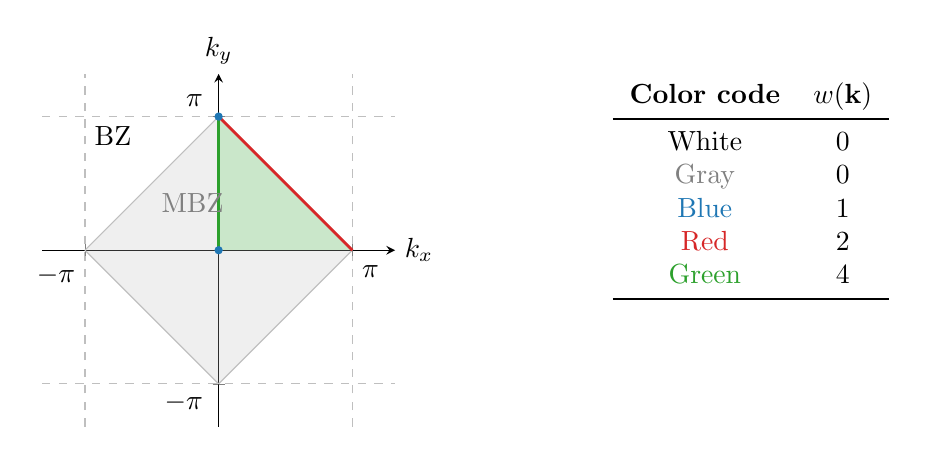
\begin{tikzpicture}
	\begin{axis}[
			axis lines=center,
			grid=both,
			grid style={color=lightgray,dashed},
			%
			xlabel={$k_x$},
			xlabel style={right},
			ylabel={$k_y$},
			ylabel style={above},
			xtick={-1},
			xticklabel={$-\pi$},
			xticklabel style={below left},
			extra x ticks={1},
			extra x tick label={$\pi$},
			extra x tick style={xticklabel style={below right}},
			ytick={-1},
			yticklabel={$-\pi$},
			yticklabel style={below left},
			extra y ticks={1},
			extra y tick label={$\pi$},
			extra y tick style={yticklabel style={above left}},
			xmin=-1.32, xmax=1.32,
			ymin=-1.32, ymax=1.32,
			%
			width=0.5\textwidth,
			height=0.5\textwidth
		]
							
        % Down paths
	    \addplot [color=lightgray,name path=D1,domain=-1:0]
	        {abs(x)-1};
	    \addplot [color=lightgray,name path=D2,domain=0:1]
	        {abs(x)-1};
	        
	    % Up paths
	    \addplot [color=lightgray,name path=U1,domain=-1:0] 
	        {-abs(x)+1};
	    \addplot [color=tabred,name path=U2,domain=0:1,line width=1] 
	        {-abs(x)+1};
	     
	    % Zero path
	    \addplot[name path=Z,domain=0:1,opacity=0]
	        {0};
	        
	    % Fill between, nodes and points
	    \addplot[color=tabgreen,opacity=0.25] 
	        fill between [of=U2 and Z];
	    \addplot[color=lightgray,opacity=0.25] 
	        fill between [of=U1 and D1];
	    \addplot[color=lightgray,opacity=0.25] 
	        fill between [of=Z and D2];
	    \draw[color=tabgreen,line width=1]
	        (axis cs:0,0) -- (axis cs:0,1);
	    \fill[color=tabblue]
			(axis cs:0,0) circle (1.5pt)
			(axis cs:0,1) circle (1.5pt);
			
		\node[anchor=north west]
		    at (-1,1) {BZ};
		\node[color=gray,anchor=north west]
		    at (-0.5,0.5) {MBZ};
	\end{axis}
	
	\node
		at (9,3) {
			\begin{tabular}{c c}
				\textbf{Color code} & $w(\mathbf{k})$ \\
					\midrule
				White & 0 \\
				{\color{gray}Gray} & 0 \\
				{\color{tabblue}Blue} & 1 \\
				{\color{tabred}Red} & 2 \\
				{\color{tabgreen}Green} & 4 \\
				\bottomrule
			\end{tabular}
		};
\end{tikzpicture}

	\caption{Graphic rendition of $s^*$-wave symmetry over the MBZ employed to optimize calculations. The right-side table indicates, for any point in BZ, the relative weight assigned to calculation.}
	\label{fig:af-mbz-s*-optimization}
\end{figure}

A very important feature when dealing with optimization is recognizing the complete $s^*$ symmetry of the model, and the HFP parameters with relative self-consistency equations. Consider Eqns.~\eqref{eq:af-renormalized-self-consistent-equation-m}, \eqref{eq:af-renormalized-self-consistent-equation-w0} and \eqref{eq:af-renormalized-self-consistent-equation-wpi}: in all of three the term inside the sum exhibits $s^*$-wave symmetry and is summed over the MBZ. Then there is no need of sweeping the entirety of the MBZ, it suffices to sweep just one fourth and just multiply coherently the result.

A little care is necessary when dealing with borders, due to MBZ nesting. Consider in fact the MBZ rhombus, sketched in gray in Fig.~\ref{fig:af-mbz-s*-optimization}: due to periodicity, two of its four boundaries must be excluded from computation in order to avoid redundancy. Let those be the lower boundaries,
\[
	k_y = \abs{k_x} - \pi
\]
Due to periodicity, the remaining upper boundaries lead to identical results, thus we may compute just one of them and multiply the result by $2$. In doing this, we need to avoid the edges: due to nesting of the MBZ, the three points
\[
	(0,\pi) \qquad (-\pi,0) \qquad (\pi,0)
\]
are the same point. Thus these need to be considered once. Looking to the bulk of the rhombus, due to $s^*$ periodicity it suffices to integrate over one quarter (considering just one internal border) and multiply by $4$. In doing this, the origin $(0,0)$ must be counted only once. Fig.~\ref{fig:af-mbz-s*-optimization} summarizes this argument: if we assign to any given point $\mathbf{k}\in\mathrm{BZ}$ a weight function $w(\mathbf{k})$ defined as in figure, in particular avoiding computations over white and gray points, we get an optimized integral over the entire MBZ saving \textit{circa} $75\%$ of runtime.

\subsection{Results of the HF algorithm at generic doping}

Within this section we will ignore stability considerations. The first set of simulations was run keeping the local repulsion fixed at a \textit{not-so-strong} coupling value, $U/t=4$, and letting $V$ vary up to a comparable value, $0 \le V/t \le 3$, for various fillings. The temperature is kept to a finite large value $\beta=100$ to avoid Fermi surface discontinuities, while lattice size is kept to a reasonably high value $L_x=L_y=256$ to suppress finite-size effects while keeping runtime low enough. The HF has been set with the following parameters:
\begin{lstlisting}[language=julia]
p::Int64 = 100						# Maximum number of iterations
dv::Dict{String,Float64} = Dict([	# Relative tolerance on each HFP
	"m" => 1e-4,
	"w0" => 1e-4,
	"wp" => 1e-4
])
dn::Float64 = 1e-2					# Relative tolerance on density
g::Float64 = 0.5					# Mixing parameter
\end{lstlisting}

\paragraph{First HFP: $m$ (magnetization).}

\begin{figure}
	\centering
	\subfloat[Non-local attraction $V/t$ depencence.]{
		\includegraphics[height=0.3\textwidth]{../Project/EHM-HartreeFock/analysis/Phase=AF/scan/Setup=B[256]/PlotOrderParameter/xVar=V/pVar=δ/m_t=1.0_U=4.0_Lx=256.0_β=100.0.pdf}
		\label{subfig:mV-scan-beta=100}
	}
	\subfloat[Doping $\delta = n-0.5$ dependence.]{
		\includegraphics[height=0.3\textwidth]{../Project/EHM-HartreeFock/analysis/Phase=AF/scan/Setup=B[256]/PlotOrderParameter/xVar=δ/pVar=V/m_t=1.0_U=4.0_Lx=256.0_β=100.0.pdf}
		\label{subfig:md-scan-beta=100}
	}	
	\caption{Plots of the magnetization $m$ in the antiferromagnetic phase as a function of both the non-local attraction $V/t$ (Fig.~\ref{subfig:mV-scan-beta=100}) and the doping $\delta = n-1/2$ (Fig.~\ref{subfig:md-scan-beta=100}), at fixed local repulsion $U/t=4$. As discussed in text, actually only $\delta=0$ simulations are stable.}
	\label{fig:mdV-scan-beta=100}
\end{figure}

Consider first Fig.~\ref{subfig:mV-scan-beta=100}. As is to be expected from Eq.~\eqref{eq:af-renormalized-self-consistent-equation-m}, being it dependent on
\[
	\Re\{\tilde{\Delta}_\mathbf{k}\} =
	m(U + 2zV)
	\qq{with $z=4$}
\]
in this renormalized antiferromagnetic phase the non-local attraction acts as a magnetization boost, essentially reproducing the same behavior of $m$ with $U$ for the conventional Hubbard model plotted in Fig.~\ref{appfig:mdU-beta=100}. The non-local attraction also enlarges the AF phase when considering various dopings, as is seen in Fig.~\ref{fig:mdV-scan-beta=100}. The magnetized region is largely extended with respect to the low-doped segment that magnetizes at $V=0$. These effects are not particularly interesting or surprising. However, something more interesting arises when looking to Fig.~\ref{fig:mUVd-heatmaps-beta=100}, a couple of heatmaps in $UV$ and $V\delta$ planes obtained respectively at $\delta=0.2$ and $U=4.0$, with $L_x$ halved down to $128$ for computational reasons. Fig.~\ref{fig:mUVd-heatmaps-beta=100} expresses again the boost to magnetization given by $V$, with a magnetized region separated by a linear boundary approximately tilted as $-1/2z$, coherently with the renormalization of $\Re\{\tilde{\Delta}_\mathbf{k}\}$. Fig.~\ref{subfig:mVd-heatmap-beta=100} in particular is interesting: a sort of shallow ``phase boundary'' appears to follow a regular sub-linear curve.

\begin{figure}
	\centering
	\subfloat[Magnetization in the $UV$ plane.]{
		\includegraphics[height=0.3\textwidth]{../Project/EHM-HartreeFock/analysis/Phase=AF/heatmap/Setup=A[128]/Heatmaps/xVar=U_yVar=V/m_t=1.0_Lx=128.0_δ=0.2_β=100.0.pdf}
		\label{subfig:mUV-heatmap-beta=100}
	}
	\subfloat[Magnetization in the $V\delta$ plane.]{
		\includegraphics[height=0.3\textwidth]{../Project/EHM-HartreeFock/analysis/Phase=AF/heatmap/Setup=B[128]/Heatmaps/xVar=V_yVar=δ/m_t=1.0_U=4.0_Lx=128.0_β=100.0.pdf}
		\label{subfig:mVd-heatmap-beta=100}
	}	
	\caption{Heatmaps of the magnetization $m$ in the antiferromagnetic phase in the $UV$ plane (Fig.~\ref{subfig:mUV-heatmap-beta=100}) and the $V\delta$ plane (Fig.~\ref{subfig:mVd-heatmap-beta=100}).}
	\label{fig:mUVd-heatmaps-beta=100}
\end{figure}

\paragraph{Second HFP: $w^{(\mathbf{0})}$ (hopping renormalization coefficient).}

\begin{figure}
	\centering
	\subfloat[Non-local attraction $V/t$ depencence.]{
		\includegraphics[height=0.3\textwidth]{../Project/EHM-HartreeFock/analysis/Phase=AF/scan/Setup=B[256]/PlotOrderParameter/xVar=V/pVar=δ/w0_t=1.0_U=4.0_Lx=256.0_β=100.0.pdf}
		\label{subfig:w0V-scan-beta=100}
	}
	\subfloat[Doping $\delta = n-0.5$ dependence.]{
		\includegraphics[height=0.3\textwidth]{../Project/EHM-HartreeFock/analysis/Phase=AF/scan/Setup=B[256]/PlotOrderParameter/xVar=δ/pVar=V/w0_t=1.0_U=4.0_Lx=256.0_β=100.0.pdf}
		\label{subfig:w0d-scan-beta=100}
	}	
	\caption{Plots of the parameter $w^{(\mathbf{0})}$ in the antiferromagnetic phase as a function of both the non-local attraction $V/t$ (Fig.~\ref{subfig:w0V-scan-beta=100}) and the doping $\delta = n-1/2$ (Fig.~\ref{subfig:w0d-scan-beta=100}), at fixed local repulsion $U/t=4$.}
	\label{fig:w0dV-scan-beta=100}
\end{figure}

Moving to the second HFP, things get interesting. Fig.~\ref{fig:w0dV-scan-beta=100} is set up as Fig.~\ref{fig:mdV-scan-beta=100}, while Fig.~\ref{fig:w0UVd-heatmaps-beta=100} as Fig.~\ref{fig:mUVd-heatmaps-beta=100}. When considering the behavior of the parameter at fixed $U$, thus looking to Fig.~\ref{subfig:w0V-scan-beta=100}, a series of \textit{plateaus} later interrupted by a continuous change in derivative are present at each doping. This is clearly evident also in Fig.~\ref{subfig:mVd-heatmap-beta=100}, with the parameter staying constant when approaching from left the maximum situated at the position of the ``phase boundary'' of Fig.~\ref{subfig:mVd-heatmap-beta=100}. The fact that there exists a geometric region of the $V\delta$ plane where are located both the phase transition and the maximum of this parameter, which controls hopping renormalization, is particularly interesting, suggesting the possibility of finding a maximally localized system by following the path extrapolated by maximizing $w^{(\mathbf{0})}$ around the phase transition.

\begin{figure}
	\centering
	\subfloat[Magnetization in the $UV$ plane.]{
		\includegraphics[height=0.3\textwidth]{../Project/EHM-HartreeFock/analysis/Phase=AF/heatmap/Setup=A[128]/Heatmaps/xVar=U_yVar=V/w0_t=1.0_Lx=128.0_δ=0.2_β=100.0.pdf}
		\label{subfig:w0UV-heatmap-beta=100}
	}
	\subfloat[Magnetization in the $V\delta$ plane.]{
		\includegraphics[height=0.3\textwidth]{../Project/EHM-HartreeFock/analysis/Phase=AF/heatmap/Setup=B[128]/Heatmaps/xVar=V_yVar=δ/w0_t=1.0_U=4.0_Lx=128.0_β=100.0.pdf}
		\label{subfig:w0Vd-heatmap-beta=100}
	}	
	\caption{Heatmaps of the parameter $w^{(\mathbf{0})}$ in the antiferromagnetic phase in the $UV$ plane (Fig.~\ref{subfig:w0UV-heatmap-beta=100}) and the $V\delta$ plane (Fig.~\ref{subfig:w0Vd-heatmap-beta=100}).}
	\label{fig:w0UVd-heatmaps-beta=100}
\end{figure}

Interestingly enough, the highly doped region, $\delta>0.4$, presents seemingly no dependency on $V$ in Fig.~\ref{subfig:w0Vd-heatmap-beta=100} (at least for thus value of $U$), as is also evident from the asymptotic behavior at increasing $V$ visible in Fig.~\ref{subfig:w0Vd-heatmap-beta=100}. Moreover, Fig.~\ref{subfig:mUV-heatmap-beta=100} and \ref{subfig:w0UV-heatmap-beta=100} appear almost reciprocal: where one parameter grows, the other is suppressed. In terms of hopping renormalization, this tells us that antiferromagnetic ordering tends to maintain $t$ non-renormalized.

\begin{figure}
	\centering
	\subfloat[Effective hopping in the $UV$ plane.]{
		\includegraphics[height=0.3\textwidth]{../Project/EHM-HartreeFock/analysis/Phase=AF/RMPs/Setup=A[128]/RMPs/xVar=U_yVar=V/t_tilde_t=1.0_Lx=128.0_δ=0.2_β=100.0.pdf}
		\label{subfig:tUV-RMP-beta=100}
	}
	\subfloat[Effective hopping in the $V\delta$ plane.]{
		\includegraphics[height=0.3\textwidth]{../Project/EHM-HartreeFock/analysis/Phase=AF/RMPs/Setup=B[128]/RMPs/xVar=V_yVar=δ/t_tilde_t=1.0_U=4.0_Lx=128.0_β=100.0.pdf}
		\label{subfig:tVd-RMP-beta=100}
	}	
	\caption{Plots of the effective hopping $\tilde{t}$ in the antiferromagnetic phase in the $UV$ plane (Fig.~\ref{subfig:tUV-RMP-beta=100}) and the $V\delta$ plane (Fig.~\ref{subfig:tVd-RMP-beta=100}).}
	\label{fig:tUVd-RMPs-beta=100}
\end{figure}

Fig.~\ref{fig:tUVd-RMPs-beta=100} reports in its subplots the renormalized hopping as a function of the model parameters, in the same setups as in the aforementioned heatmaps. As is depicted, the NN interaction $V$ tends to reduce effective hopping amplitude down to a significant fraction of the starting value: $t$ is damped of a $30\%$ factor or so. As is evident from Fig.~\ref{subfig:tVd-RMP-beta=100}, for a small local repulsion $U=4$ the value of $\tilde{t}$ lowers as the doping grows, reaching a maximum approximately on the position of the maxima of $w^{(\mathbf{0})}$ in Fig.~\ref{subfig:w0Vd-heatmap-beta=100}, which was expected considering Eq.~\eqref{eq:af-fock-hop-ss-renormalization}.

\paragraph{Third HFP: $w^{(\bm{\pi})}$ (imaginary gap coefficient).}

Unsurprisingly, the third HFP turns out to be essentially zero in all parameters space, considering also numerical fluctuations. This was expected: when deriving the MF solution to the model within AF phase, we essentially reduced it to the already known solution of Sec.~\ref{appsec:antiferromagnetic-phase}. The gap there was a real parameter, thus by purely renormalizing the parameters obtained within such solution there is no need for the present gap to acquire a non-zero imaginary part.

\subsection{Role of hopping renormalization: switching off $w^{(\mathbf{0})}$}
\todo

%\def\GraphicsFolder{parts/mft-analysis/chapters/superconducting-instability/pictures}
\chapter{Superconducting instability}\label{chap:mft-su-instability}

This chapter is devoted to studying the superconducting phase of the system. The only symmetry we assume to break is the $\mathrm{U}^\mathrm{c}(1)$ charge symmetry, thus allowing for superconducting fluctuations. As is described thoroughly in Sec.~\ref{subsec:fock-renormalization-hopping-amplitude}, the hopping amplitude is renormalized because of the non-local attraction. The symmetry structure of the pairing mechanism determines the contributing Cooper fluctuations: for $s$-wave and $d$-wave superconductivity, only the o.s. Cooper term contributes; for $p_\ell$-wave superconductivity, the s.s. term contributes as well. In the following sections, a derivation containing both Cooper terms is proposed.

{\color{tabred}[
	To be continued: separate singlet and triplet pairing channels, and describe them separately by the means of four-components Nambu spinors. Use selection rules to set $\Delta^{(p_\ell)}=0$ in the singlet channel, in order to justify results obtained by a pure space-even simulation containing just the o.s. terms.
	]}

\section{Cooper fluctuations in the EHM}

Let us start once again from the general EHM of Eq.~\eqref{eq:extended-hubbard-model},
\[
	\hat H =
	\underbrace{
		-t \sum_{\langle ij \rangle} \sum_\sigma \hat c_{i\sigma}^\dagger \hat c_{j\sigma}
	}_{\hat H_t} \underbrace{
		+U \sum_i \hat c_{i\uparrow}^\dagger \hat c_{i\downarrow}^\dagger \hat c_{i\downarrow} \hat c_{i\uparrow}
		\vphantom{
			\sum_{\langle ij \rangle}
		}
	}_{\hat H_U}
	\underbrace{
		- V \sum_{\langle ij \rangle} \sum_{\sigma \sigma'} \hat c_{i\sigma}^\dagger \hat c_{j\sigma'}^\dagger \hat c_{j\sigma'} \hat c_{i\sigma}
	}_{\hat H_V}
\]
As is discussed in Sec.~\ref{sec:mft-discussion-non-local-source}, when applying Wick's theorem the resulting terms break the natural symmetries of the model. The superconducting symmetry we study breaks just the $\mathrm{U}^\mathrm{c}(1)$ charge conservation. Now, when dealing with superconducting Cooper pairing we need to account also for the spatial structure of the Cooper pair itself. Consider the generic Cooper fluctuation
\[
	\big\langle
		\hat c_{i\sigma}^\dagger \hat c_{j\sigma'}^\dagger
	\big\rangle
	\qq{with $i,j$ NN}
\]
From basic Quantum Mechanics we know the summation rules of the spin algebra $\mathfrak{su}(2)$,
\[
	\frac 1 2 \otimes \frac 1 2 = 0 \oplus 1
\]
The two pairing channels are, at this level, the singlet channel associated to total spin $0$ and the triplet channel associated to total spin $1$. If we impose a specific spatial symmetry on the hamiltonian the ground state wavefunction will follow naturally, and the pairing channel will be the one providing a total anti-symmetry to the full wavefunction. This gives a selection rule over the relevant pairings: if we work with space symmetric structures -- say, $s^*$-wave or $d$-wave -- the pairing will happen in singlet channel, allowing us to eliminate the triplet pairing. This concept is summarized in Tab.~\ref{tab:su-pairings-symmetry-structures}.

\begin{table}
	\centering
	\begin{tabular}{c c c}
		\textbf{Spatial structure} & \textbf{Pairing channel} & \textbf{Relevant pairing} \\
		\midrule
		Symmetric wave function & Singlet pairing & Just $\displaystyle \big\langle
		\hat c_{i\sigma}^\dagger \hat c_{j\overline{\sigma}}^\dagger
		\big\rangle$ \\
		Anti-symmetric wave function & Triplet pairing & Both $\displaystyle \big\langle
		\hat c_{i\sigma}^\dagger \hat c_{j\overline{\sigma}}^\dagger
		\big\rangle$ and $\displaystyle \big\langle
		\hat c_{i\sigma}^\dagger \hat c_{j\sigma}^\dagger
		\big\rangle$
	\end{tabular}
	\caption{Relation of the Cooper pairing channell with the wavefunction spatial symmetry (intended as the inversion $(x,y) \to (-x,-y)$).}
	\label{tab:su-pairings-symmetry-structures}
\end{table}

{\color{tabred}[ Add: Cooper pairing considerations in the pure Hubbard model. ]}

\section{Cooper fluctuations in the opposite-spin sector}

This section deals with Cooper fluctuations induced by the o.s. part of the non-local hamiltonian --referring to the notation of Eq.~\eqref{eq:ehm-non-local-ss-os-terms}-- somewhat the simplest form of Cooper pairing. This sector contributes both to singlet pairing and triplet pairing. Considering Cooper fluctuations in the singlet channel, we need to break $\mathrm{U}^\mathrm{c}(1)$ symmetry imposing space inversion symmetry, while for the triplet anti-symmetry is required. Let us now break down the MFT discussion for the local and non-local interactions.

\paragraph{Local interaction $U$.}

Consider first the local part,
\[
	\hat H_U = U \sum_{i \in \mathcal{S}} \hat n_{i\uparrow} \hat n_{i\downarrow} \simeq U \sum_{i \in \mathcal{S}} \left[
		\big\langle
			\hat c_{i\uparrow}^\dagger \hat c_{i\downarrow}^\dagger
		\big\rangle
		\hat c_{i\downarrow} \hat c_{i\uparrow} + \hat c_{i\uparrow}^\dagger \hat c_{i\downarrow}^\dagger \big\langle
			\hat c_{i\downarrow} \hat c_{i\uparrow}
		\big\rangle
	\right]
\]
and use the result of Eq.~\eqref{eq:reciprocal-space-local-interaction-explicit},
\[
	\hat H_U \simeq \frac{U}{L_x L_y}
	\sum_{\mathbf{K}, \mathbf{k}, \mathbf{k}'}
	\left[
		\big\langle
			\hat c_{\mathbf{K}+\mathbf{k} \uparrow}^\dagger \hat c_{\mathbf{K}-\mathbf{k} \downarrow}^\dagger
		\big\rangle
		\hat c_{\mathbf{K}-\mathbf{k}' \downarrow} \hat c_{\mathbf{K}+\mathbf{k}' \uparrow} +
		\hat c_{\mathbf{K}+\mathbf{k} \uparrow}^\dagger \hat c_{\mathbf{K}-\mathbf{k} \downarrow}^\dagger
		\big\langle
			\hat c_{\mathbf{K}-\mathbf{k}' \downarrow} \hat c_{\mathbf{K}+\mathbf{k}' \uparrow}
		\big\rangle
	\right]
\]
We are not breaking translational invariance, thus only Cooper fluctuations with net zero total momentum are allowed. This means only $\mathbf{K}=\mathbf{0}$ contributes. Define the pairing operator 
\[
	\hat \phi_\mathbf{k} \equiv \hat c_{-\mathbf{k}\downarrow} \hat c_{\mathbf{k} \uparrow}
	\qquad
	\hat \phi_\mathbf{k}^\dagger \equiv \hat c_{\mathbf{k} \uparrow}^\dagger \hat c_{-\mathbf{k}\downarrow}^\dagger
\]
Then the non local repulsion reduces to the ordinary BCS-like interaction,
\begin{equation}\label{eq:su-ugap-mft}
	\hat H_U \simeq \sum_\mathbf{k} \left[
		\mathcal{U}_\mathbf{k} \hat \phi_\mathbf{k} + \mathcal{U}_\mathbf{k}^* \hat \phi_\mathbf{k}^\dagger
	\right]
\end{equation}
where the MFT parameter $\mathcal{U}_\mathbf{k}$ must satisfy the self-consistency equation
\begin{equation}\label{eq:su-ugap-self-consistency}
	\mathcal{U}_\mathbf{k} \equiv \frac{U}{L_x L_y} \sum_\mathbf{k} \big\langle 
		\hat \phi_\mathbf{k}^\dagger
	\big\rangle
\end{equation}
Note that $\mathcal{U}_\mathbf{k}$ is actually momentum independent. This is due to the fact that the repulsion is completely localized.

\paragraph{Non-local interaction $V$.}

The non-local attraction in the opposite-spin sector of $\hat H_V$ is given by
\[
	\hat H_V^{(\mathrm{o.s.})} = -V \sum_{\ev{ij}} \sum_\sigma \hat n_{i\sigma} \hat n_{j\overline{\sigma}}
\]
which, using Eq.~\eqref{eq:ehm-mft-nonlocal-opposite-spin} and performing Wick's contractions, reduces to:
\[
\begin{aligned}
	\hat H_V^{(\mathrm{o.s.})} &= -V \sum_{i \in \mathcal{S}} \sum_{\ell = x,y} \sum_{\delta = \pm \delta_\ell}
	\hat n_{i\uparrow} \hat n_{i+\delta \downarrow} \\
	&\simeq - V \sum_{i \in \mathcal{S}} \sum_{\ell = x,y} \sum_{\delta = \pm \delta_\ell} \left[
		\langle 
			\hat c_{i\uparrow}^\dagger \hat c_{i + \delta \downarrow}^\dagger
		\rangle
		\hat c_{i + \delta \downarrow} \hat c_{i\uparrow} 
		+
		\hat c_{i\uparrow}^\dagger \hat c_{i + \delta \downarrow}^\dagger
		\langle
			\hat c_{i + \delta \downarrow} \hat c_{i\uparrow} 
		\rangle
	\right]
\end{aligned}
\]
Using Eq.~\eqref{eq:reciprocal-space-non-local-interaction-explicit} we can move to reciprocal space,
\begin{multline*}
	\hat H_V^{(\mathrm{o.s.})} \simeq -\frac{V}{L_x L_y}
	\sum_{\mathbf{K}, \mathbf{k}, \mathbf{k}'} \left[
		\cos \left(
			\delta k_x
		\right)	+ \cos \left(
			\delta k_y
		\right)	
	\right]	\\
	\times \left[ 
		\big\langle
			\hat c_{\mathbf{K}+\mathbf{k} \uparrow}^\dagger \hat c_{\mathbf{K}-\mathbf{k} \downarrow}^\dagger
		\big\rangle 
		\hat c_{\mathbf{K}-\mathbf{k}' \downarrow} \hat c_{\mathbf{K}+\mathbf{k}'\uparrow} 
		+
		\hat c_{\mathbf{K}+\mathbf{k} \uparrow}^\dagger \hat c_{\mathbf{K}-\mathbf{k} \downarrow}^\dagger
		\big\langle 
			\hat c_{\mathbf{K}-\mathbf{k}' \downarrow} \hat c_{\mathbf{K}+\mathbf{k}'\uparrow}
		\big\rangle
	\right]
\end{multline*}
Identical considerations as above hold, and just the $\mathbf{K}=\mathbf{0}$ term contributes. We have finally
\[
\begin{aligned}
	\hat H_V^{(\mathrm{o.s.})} \simeq - \sum_{\mathbf{k}, \mathbf{k}'}
	V_{\mathbf{k}\mathbf{k}'} \left[
	\langle 
	\hat \phi_\mathbf{k}^\dagger
	\rangle \hat \phi_{\mathbf{k}'} + \langle 
	\hat \phi_\mathbf{k}
	\rangle \hat \phi_{\mathbf{k}'}^\dagger
	\right]	
\end{aligned}
\]
where the two-body potential was defined
\[
	V_{\mathbf{k}\mathbf{k}'} = \frac{V}{L_x L_y} \left[
		\cos \left(
			\delta k_x
		\right)	+ \cos \left(
			\delta k_y
		\right)	
	\right]
\]
Making use of the decomposition of Eq.~\eqref{eq:coscos-symmetries-decomposition}, the two-body potential becomes
\[
\begin{aligned}
	V_{\mathbf{k}\mathbf{k}'} &= \frac{V}{2L_xL_y} \sum_\gamma \varphi_\mathbf{k}^{(\gamma)} \varphi_{\mathbf{k}'}^{(\gamma)*} \\
	&= \sum_\gamma V^{(\gamma)} \varphi_\mathbf{k}^{(\gamma)} \varphi_{\mathbf{k}'}^{(\gamma)*} \\
\end{aligned}
\]
being $\gamma \in \lbrace s^*, p_x, p_y, d_{x^2-y^2} \rbrace$ and $\varphi_\mathbf{k}^{(\gamma)}$ the reciprocal-space expressions for the form factors of Tab.~\ref{tab:x-wave-real-factors}, listed explicitly in Tab.~\ref{tab:x-wave-reciprocal-factors}, and $V_{\mathbf{k}\mathbf{k}'}^{(\gamma)}$ the symmetry-resolved components of the non-local attraction. Then the two-body potential has been decomposed in its planar symmetry components, each of which will naturally couple only to identically structured parameters in the full hamiltonian.

Define now the non-local gap function
\begin{equation}\label{eq:su-ugap-self-consistency-intermediate}
	\mathcal{V}_\mathbf{k} \equiv \sum_{\mathbf{k}'}
	V_{\mathbf{k}\mathbf{k}'}
	\langle
	\hat \phi_{\mathbf{k}'}^\dagger
	\rangle
\end{equation}
one gets immediately
\begin{equation}\label{eq:su-vgap-mft}
	\hat H_V \simeq -\sum_\mathbf{k} \left[
	\mathcal{V}_\mathbf{k} \hat \phi_\mathbf{k} + \mathcal{V}_\mathbf{k}^* \hat \phi_\mathbf{k}^\dagger
	\right]	
\end{equation}
To assume symmetry is broken in a specific symmetry channel $\gamma$ means precisely to assume $\langle \hat \phi_\mathbf{k} \rangle \propto \varphi_\mathbf{k}^{(\gamma)}$. Of course, in Eq.~\eqref{eq:su-ugap-self-consistency-intermediate} only the $\gamma$ component of the potential survives, implying the gap function acquires the same symmetry,
\[
	\mathcal{V}_\mathbf{k} \propto \sum_{\mathbf{k}'} \varphi_\mathbf{k}^{(\gamma)} \varphi_{\mathbf{k}'}^{(\gamma)*}
	\varphi_{\mathbf{k}'}^{(\gamma)} \propto \varphi_\mathbf{k}^{(\gamma)}
\]
where orthonormality of the $\varphi_\mathbf{k}^{(\gamma)}$ functions of Tab.~\ref{tab:x-wave-reciprocal-factors} was used. Thus, assuming to have superconductivity in a given sector $\gamma$, the self consistency equation reads
\begin{equation}\label{eq:su-vgap-self-consistency}
	\forall \gamma \in \lbrace s^*, p_x, p_y, d_{x^2-y^2} \rbrace
	\qquad
	\mathcal{V}_\mathbf{k}\big|_\gamma \equiv \frac{V}{2L_x L_y} \sum_\mathbf{k}
	\varphi_\mathbf{k}^{(\gamma)}
	\big\langle 
		\hat \phi_\mathbf{k}^\dagger
	\big\rangle
\end{equation}
Now we merge the two interaction in a single gap function.

\subsection{Full gap function and self-consistency equations}

Define the full gap function as the sum of both contributions,
\begin{equation}\label{eq:su-os-gap-function-definition}
	\Delta_\mathbf{k} \equiv \mathcal{V}_\mathbf{k} - \mathcal{U}_\mathbf{k}
\end{equation}
The full self-consistency equation is given by the simple combination of Eqns.~\eqref{eq:su-ugap-self-consistency} and \eqref{eq:su-vgap-self-consistency},
\begin{equation}\label{eq:self-consistency-equation}
	\Delta_\mathbf{k} \equiv \sum_{\mathbf{k}'}
	\left[
		V^{(s)} +
		V_{\mathbf{k}\mathbf{k}'}
	\right]
	\langle
		\hat \phi_{\mathbf{k}'}^\dagger
	\rangle
	\qq{with}
	V^{(s)} = - \frac{U}{2L_xL_y}
\end{equation}
The gap function decomposes in symmetry channels as well,
\[
\Delta_\mathbf{k} = \sum_\gamma \Delta^{(\gamma)} \varphi_\mathbf{k}^{(\gamma)}
\]
If SC arises in a specific symmetry channel, $\Delta_\mathbf{k}$ will show the same symmetry. It follows, due to orthonormality and using Eq.~\eqref{eq:self-consistency-equation},
\begin{align}
	\Delta^{(\gamma)} &= \frac{1}{L_xL_y} \sum_{\mathbf{k}} \varphi_\mathbf{k}^{(\gamma)*} \Delta_\mathbf{k} \nonumber \\
	&= \frac{1}{L_xL_y} \sum_{\mathbf{k}} \varphi_\mathbf{k}^{(\gamma)*} \sum_{\mathbf{k}'}
	\left[
	V^{(s)} +
	V_{\mathbf{k}\mathbf{k}'}
	\right]
	\langle
	\hat \phi_{\mathbf{k}'}^\dagger
	\rangle \nonumber \\
	&= \frac{1}{L_xL_y} \sum_{\mathbf{k}} \varphi_\mathbf{k}^{(\gamma)*} \sum_{\mathbf{k}'\gamma'}
	V^{(\gamma')} \varphi_\mathbf{k}^{(\gamma')} \varphi_{\mathbf{k}'}^{(\gamma')*}
	\langle
	\hat \phi_{\mathbf{k}'}^\dagger
	\rangle \nonumber \\
	&= V^{(\gamma)} \sum_{\mathbf{k}} \varphi_\mathbf{k}^{(\gamma)*} \langle
	\hat \phi_{\mathbf{k}}^\dagger
	\rangle \label{eq:self-consistency-equation-explicit}
\end{align}
This result provides a set of self-consistency equations for each symmetry channel, listed in Tab.~\ref{tab:x-wave-self-consistency-equation}. Notice that to reconstruct self-consistently the full $s$-wave phase transition, the actual gap function is given by
\[
\Delta^{(s)} + \Delta^{(s^*)} (c_x + c_y)
\]
The $s$-wave transition is the only one equipped of both the local and the non-local parts.

\setlength{\extrarowheight}{1em}
\begin{table}
	\centering
	\begin{tabular}{r E l l}
		\textbf{Structure} & \multicolumn{2}{c}{\textbf{Self-consistency equation}} & \textbf{Graph} \\
		\midrule
		$s$-wave & $\Delta^{(s)}$ & $\displaystyle -\frac{U}{2L_xL_y} \sum_{\mathbf{k}} \langle
		\hat \phi_{\mathbf{k}}^\dagger
		\rangle $ & Fig.~\ref{subfig:s-wave-correlator} \\
		Extended $s$-wave & $\Delta^{(s^*)}$ & $\displaystyle \frac{V}{L_xL_y} \sum_{\mathbf{k}} (c_x + c_y) \langle
		\hat \phi_{\mathbf{k}}^\dagger
		\rangle$ & Fig.~\ref{subfig:s*-wave-correlator} \\
		$p_x$-wave & $\Delta^{(p_x)}$ & $\displaystyle - i\sqrt{2} \frac{V}{L_xL_y} \sum_{\mathbf{k}} s_x \langle
		\hat \phi_{\mathbf{k}}^\dagger
		\rangle$ & Fig.~\ref{subfig:px-wave-correlator} \\
		$p_y$-wave & $\Delta^{(p_y)}$ & $\displaystyle -i \sqrt{2} \frac{V}{L_xL_y} \sum_{\mathbf{k}} s_y \langle
		\hat \phi_{\mathbf{k}}^\dagger
		\rangle$ & Fig.~\ref{subfig:py-wave-correlator} \\
		$d_{x^2-y^2}$-wave & $\Delta^{(d)}$ & $\displaystyle \frac{V}{L_xL_y} \sum_{\mathbf{k}} (c_x - c_y) \langle
		\hat \phi_{\mathbf{k}}^\dagger
		\rangle$ & Fig.~\ref{subfig:d-wave-correlator} 
	\end{tabular}
	\caption{Symmetry resolved self-consistency equations for the MFT parameters $\Delta^{(\gamma)}$, based on Eq.~\eqref{eq:self-consistency-equation} and \eqref{eq:self-consistency-equation-explicit}. By computing $\langle \hat \phi_{\mathbf{k}}^\dagger \rangle$, it is possible to reconstruct the various components of the gap function.}
	\label{tab:x-wave-self-consistency-equation}
\end{table}
\setlength{\extrarowheight}{0em}

\subsection{Non-local bands renormalization in the same-spin sector}\label{subsec:su-bands-renormalization-1}

In the context of antiferromagnetism (Sec.~\ref{subsec:fock-renormalization-hopping-amplitude}) we discussed the role of the non-local interaction $\hat H_V$ as a source of bands effective renormalization. One of the most interesting results was the on of Eq.~\eqref{eq:af-fock-hop-ss-renormalization}, with the hopping parameter being rigidly shifted. In the present context, we aim to treat the non-local part similarly by using immediately the aforementioned results. Start from Eq.~\eqref{eq:reciprocal-space-non-local-interaction-fock-intermediate},
\begin{multline*}
	V \sum_{\ev{ij}} \sum_\sigma \left[
	\langle
	\hat c_{i\sigma}^\dagger \hat c_{j\sigma}
	\rangle \hat c_{j\sigma}^\dagger  \hat c_{i\sigma} + \hc
	\right] \\
	= \frac{2V}{L_x L_y} \sum_{\mathbf{K}, \mathbf{k}, \mathbf{k}'} \sum_\sigma \left[
	\cos \left(
	\delta k_x
	\right)	+ \cos \left(
	\delta k_y
	\right)	
	\right]	
	\langle
	\hat c_{\mathbf{K}+\mathbf{k} \sigma}^\dagger 
	\hat c_{\mathbf{K}-\mathbf{k}' \sigma}
	\rangle
	\hat c_{\mathbf{K}-\mathbf{k} \sigma}^\dagger  \hat c_{\mathbf{K}+\mathbf{k}'\sigma}
\end{multline*}
For the BCS ground state, it is immediate to see the only relevant contribution comes from
\[
	\mathbf{k} = -\mathbf{k}'
\]
which gives the diagonal part of Eq.~\eqref{eq:reciprocal-space-non-local-interaction-fock-intermediate-2}. We are then left with (half) the result of Eq.~\eqref{eq:reciprocal-space-non-local-interaction-fock-dd-intermediate}
\begin{equation}\label{eq:reciprocal-space-non-local-interaction-fock-dd-intermediate-su}
	V \sum_{\ev{ij}} \sum_\sigma \left[
	\langle
	\hat c_{i\sigma}^\dagger \hat c_{j\sigma}
	\rangle \hat c_{j\sigma}^\dagger  \hat c_{i\sigma} + \hc
	\right]	= \frac{2V}{L_x L_y} \sum_{\mathbf{q}, \mathbf{q}'} \sum_\sigma \left[
	\cos \left( \delta q_x \right) + \cos \left( \delta q_y \right)	
	\right] \langle
	\hat c_{\mathbf{q}\sigma}^\dagger  \hat c_{\mathbf{q}\sigma}
	\rangle
	\hat c_{\mathbf{q}'\sigma}^\dagger  \hat c_{\mathbf{q}'\sigma}
\end{equation}
Recall Eq.~\eqref{eq:coscos-symmetries-decomposition}: the structure term decomposes in harmonic waves, and this feature is particularly handy in order to decouple the $\mathbf{q}$ and $\mathbf{q}'$ parts, as we later do.

\section{Superconducting solution in the Nambu formalism}

As a first approach to anisotropic SC in the Hubbard model, let us discuss the superconducting solutions in the simple scenario where crystal translational invariance is preserved and thus the system can be treated by the means of common BCS. As will be discussed, the non-local attraction acts as a source of SC in all symmetry sectors.

Define the Nambu spinor\footnote{
	Notice that the spinor is here differently defined with respect to App.~\ref{appendix:mean-field-hubbard}, where because of the HF prevalence in mean-field decoupling the spinor components were homogeneously fermions creations or destructions.
} as in BCS
\[
\hat \Psi_\mathbf{k} \equiv \begin{bmatrix}
	\hat c_{\mathbf{k}\uparrow} \\
	\hat c_{-\mathbf{k}\downarrow}^\dagger
\end{bmatrix}
\]
Evidently,
\begin{equation}\label{eq:extended-hubbard-phi-psi-expressions}
	\phi_\mathbf{k} = \hat \Psi_\mathbf{k}^\dagger \begin{bmatrix}
		0 & 1 \\ 0 & 0
	\end{bmatrix} \hat \Psi_\mathbf{k}
	\qquad
	\phi_\mathbf{k}^\dagger = \hat \Psi_\mathbf{k}^\dagger \begin{bmatrix}
		0 & 0 \\ 1 & 0
	\end{bmatrix} \hat \Psi_\mathbf{k}
\end{equation}
The full hamiltonian is then given by:
\begin{equation}\label{eq:extended-hubbard-hamiltonian-nambu-bogoliubov}
	\hat H = \sum_\mathbf{k} \hat \Psi_\mathbf{k} h_\mathbf{k} \hat \Psi_\mathbf{k}
	\qquad
	h_\mathbf{k} \equiv \begin{bmatrix}
		\epsilon_\mathbf{k} & - \Delta_\mathbf{k}^* \\
		- \Delta_\mathbf{k} & - \epsilon_\mathbf{k}
	\end{bmatrix}
\end{equation}
Next step is to perform the well-known Bogoliubov transform and reduce all the problem down to a simple ensemble of quantum pseudospins.

\subsection{Bogoliubov transform and pseudospins picture}\label{subsec:bogoliubov-mean-field-extended-hubbard}

Let $\tau^\alpha$ for $\alpha = x,y,z$ be the Pauli matrices. Define the pseudospin operator:
\[
	\hat s_\mathbf{k}^\alpha \equiv \hat \Psi_\mathbf{k}^\dagger \tau^\alpha \hat \Psi_\mathbf{k}
	\qq{for}
	\alpha = x,y,z
\]
As can be shown easily, these operators realize spin-$1/2$ algebra. $\hat H$ represents an ensemble of $L_x L_y$ independent spins subject to pseudo-magnetic fields. Note that, differently form App.~\ref{app:mean-field-hubbard} where the chemical potential is inserted later (because in Nambu formalism it accounts for a diagonal term) here the chemical potential is part of the $z$ component of the pseudo-magnetic field, since
\begin{align}
	\hat n_{\mathbf{k}\uparrow} + \hat n_{-\mathbf{k}\downarrow} &= \hat c_{\mathbf{k}\uparrow}^\dagger \hat c_{\mathbf{k}\uparrow} + \hat c_{-\mathbf{k}\downarrow}^\dagger \hat c_{-\mathbf{k}\downarrow} \\
	&= \hat c_{\mathbf{k}\uparrow}^\dagger \hat c_{\mathbf{k}\uparrow} - \hat c_{-\mathbf{k}\downarrow} \hat c_{-\mathbf{k}\downarrow}^\dagger + \Id \nonumber \\
	&=  \hat \Psi_\mathbf{k}^\dagger \tau^z \hat \Psi_\mathbf{k} + \Id \label{eq:number-operator-z-spin-relation}
\end{align}
and then it follows
\[
\begin{aligned}
	-\mu\hat N &= -\mu \sum_{\mathbf{k} \in \mathrm{BZ}} \left[ 
	\hat n_{\mathbf{k}\uparrow} + \hat n_{-\mathbf{k}\downarrow} 
	\right] \\
	&= -\mu \sum_{\mathbf{k} \in \mathrm{BZ}} \hat \Psi_\mathbf{k}^\dagger \tau^z \hat \Psi_\mathbf{k} -\mu L_x L_y
\end{aligned}
\]
Then, adding a term $-\mu \hat N$ to $\hat H$, apart from an irrelevant total energy increase, changes the pseudo-field whose explicit form becomes
\begin{equation} \label{eq:extended-hubbard-pseudo-magnetic-field}
	\mathbf{b}_\mathbf{k} \equiv \begin{bmatrix}
		-\Re{\Delta_\mathbf{k}} \\
		-\Im{\Delta_\mathbf{k}} \\ \epsilon_\mathbf{k} - \mu
	\end{bmatrix}
\end{equation}
This hamiltonian behaves as an ensemble of spins in local magnetic fields precisely as in Eq.~\eqref{appeq:hubbard-bogoliubov-hamiltonian-pseudofields},
\begin{equation}\label{eq:extended-hubbard-bogoliubov-hamiltonian-pseudofields}
	\hat H -\mu \hat N = \sum_{\mathbf{k} \in \mathrm{BZ}} \mathbf{b}_\mathbf{k} \cdot \hat{\mathbf{s}}_\mathbf{k}
	\qq{where}
	\hat{\mathbf{s}}_\mathbf{k} = \begin{bmatrix}
		\hat s_\mathbf{k}^x \\
		\hat s_\mathbf{k}^y \\
		\hat s_\mathbf{k}^z
	\end{bmatrix}
\end{equation}
Proceed as in App.~\ref{app:mean-field-hubbard} and diagonalize via a rotation,
\[
d_\mathbf{k} \equiv \begin{bmatrix}
	-E_\mathbf{k} & \\ & E_\mathbf{k}
\end{bmatrix}
\qq{being}
E_\mathbf{k} \equiv \sqrt{\xi_\mathbf{k}^2 + \abs{\Delta_\mathbf{k}}^2}
\]
and $\xi_\mathbf{k} \equiv \epsilon_\mathbf{k} - \mu$. Given the pseudoangles
\[
\tan(2\theta_\mathbf{k}) \equiv \frac{\abs{\Delta_\mathbf{k}}}{\xi_\mathbf{k}}
\qquad
\tan(2\zeta_\mathbf{k}) \equiv \frac{\Im{\Delta_\mathbf{k}}}{\Re{\Delta_\mathbf{k}}}
\]
the general diagonalizer will be an orthogonal rotation matrix
\begin{align}
	W_\mathbf{k} &= e^{i \left(\theta_\mathbf{k} - \frac{\pi}{2}\right) \tau^y} e^{i \zeta_\mathbf{k} \tau^z} \nonumber \\
	&= \begin{bmatrix}
		-\sin\theta_\mathbf{k}  & -\cos\theta_\mathbf{k}  \\ 
		\cos\theta_\mathbf{k}  & -\sin\theta_\mathbf{k} 
	\end{bmatrix} \begin{bmatrix}
		e^{i\zeta_\mathbf{k} } & \\ & e^{-i\zeta_\mathbf{k} }
	\end{bmatrix} \nonumber \\
	&= \begin{bmatrix}
		-\sin\theta_\mathbf{k}  e^{i\zeta_\mathbf{k} } & -\cos\theta_\mathbf{k}  e^{-i\zeta_\mathbf{k} }  \\ 
		\cos\theta_\mathbf{k}  e^{i\zeta_\mathbf{k} } & -\sin\theta_\mathbf{k}  e^{-i\zeta_\mathbf{k} } 
	\end{bmatrix} \label{eq:extended-hubbard-bogoliubov-W-diagonalizer-explicit}
\end{align}
given by a rotation of angle $\zeta_\mathbf{k}$ around the $z$ axis, to align the $x$ axis with the field projection onto the $xy$ plane, followed by a rotation around the $y$ axis to anti-align with the pseudo-field. 

\subsection{BCS ground state properties}

The MFT-BCS solution is given by a degenerate Fermi gas at ground state, whose quasi-particles occupy two bands $\pm E_\mathbf{k}$ and their fermionic operators are given by
\[
	\hat \gamma_\mathbf{k}^{(-)} \equiv \left[
		W_\mathbf{k} \hat \Psi_\mathbf{k}
	\right]_1
	\qquad
	\hat \gamma_\mathbf{k}^{(+)} \equiv \left[
		W_\mathbf{k} \hat \Psi_\mathbf{k}
	\right]_2
\]
The diagonalization operators are given by
\[
	\hat\Gamma_\mathbf{k} \equiv W_\mathbf{k} \hat\Psi_\mathbf{k}
	\qq{where}
	\hat\Gamma_\mathbf{k} = \begin{bmatrix}
		\hat \gamma_\mathbf{k}^{(-)} \\ \hat \gamma_\mathbf{k}^{(+)}
	\end{bmatrix}
\]
Using Eq.~\eqref{appeq:finite-temperature-order-parameter-derivation-intermediate}, 
\[
	\left\langle [\hat \Psi_\mathbf{k}^\dagger]_i [\hat \Psi_\mathbf{k}]_j \right\rangle = [W_\mathbf{k}]_{1 i} [W_\mathbf{k}^\dagger]_{j 1} f\left( -E_\mathbf{k}; \beta,0 \right) + [W_\mathbf{k}]_{2 i} [W_\mathbf{k}^\dagger]_{j 2} f\left( E_\mathbf{k}; \beta,0 \right)
\]
where in the Fermi-Dirac function chemical potential was set to zero, because it already was included in the diagonalized hamiltonian.
Recalling Eq.~\eqref{eq:extended-hubbard-phi-psi-expression}, it follows for $i=1$, $j=2$
\begin{align}
	\langle \hat \phi_\mathbf{k}^\dagger \rangle &= [W_\mathbf{k}]_{11} [W_\mathbf{k}^\dagger]_{21} f\left( -E_\mathbf{k}; \beta,0 \right) + [W_\mathbf{k}]_{21} [W_\mathbf{k}^\dagger]_{22} f\left( E_\mathbf{k}; \beta,0 \right) \label{eq:pairing-dagger-expectation-algorithmic} \\
	&= \frac{1}{2} \sin \left(
	2 \theta_\mathbf{k}
	\right) e^{i 2 \zeta_\mathbf{k}} \tanh(\frac{\beta E_\mathbf{k}}{2}) \label{eq:pairing-dagger-expectation-theoretical}
\end{align}
The last passage has been obtained by computing the matrix element from the explicit form of $W_\mathbf{k}$ of Eq.~\eqref{eq:extended-hubbard-bogoliubov-W-diagonalizer-explicit} and by the simple relation
\[
\begin{aligned}
	\frac{1}{e^{-x}+1} - \frac{1}{e^x+1} &= \frac{e^x -1}{e^x +1} \\
	&= \tanh(\frac{x}{2})
\end{aligned}
\]
Similarly, for $i=1$, $j=1$
\begin{align}
	\langle \hat c_{\mathbf{k}\uparrow}^\dagger \hat c_{\mathbf{k}\uparrow} \rangle &= [W_\mathbf{k}]_{11} [W_\mathbf{k}^\dagger]_{11} f\left( -E_\mathbf{k}; \beta,0 \right) + [W_\mathbf{k}]_{21} [W_\mathbf{k}^\dagger]_{12} f\left( E_\mathbf{k}; \beta,0 \right) \label{eq:number-dagger-expectation-algorithmic-11} \\
	&= \sin^2 \theta_\mathbf{k} f\left( -E_\mathbf{k}; \beta,0 \right) + \cos^2 \theta_\mathbf{k} f\left( E_\mathbf{k}; \beta,0 \right) \nonumber \\
	&= \sin^2 \theta_\mathbf{k} \tanh(\frac{\beta E_\mathbf{k}}{2}) + f\left( E_\mathbf{k}; \beta,0 \right)
	\label{eq:number-dagger-expectation-theoretical-11}
\end{align}
and for $i=2$, $j=2$
\begin{align}
	\langle \hat c_{-\mathbf{k}\downarrow} \hat c_{-\mathbf{k}\downarrow}^\dagger \rangle &= [W_\mathbf{k}]_{12} [W_\mathbf{k}^\dagger]_{21} f\left( -E_\mathbf{k}; \beta,0 \right) + [W_\mathbf{k}]_{22} [W_\mathbf{k}^\dagger]_{22} f\left( E_\mathbf{k}; \beta,0 \right) \label{eq:number-dagger-expectation-algorithmic-22} \\
	&= \cos^2 \theta_\mathbf{k} f\left( -E_\mathbf{k}; \beta,0 \right) + \sin^2 \theta_\mathbf{k} f\left( E_\mathbf{k}; \beta,0 \right) \nonumber \\
	&= \cos^2 \theta_\mathbf{k} \tanh(\frac{\beta E_\mathbf{k}}{2}) + f\left( E_\mathbf{k}; \beta,0 \right)
	\label{eq:number-dagger-expectation-theoretical-22}
\end{align}

\paragraph{Gap function.} Eqns.~\eqref{eq:pairing-dagger-expectation-algorithmic}, \eqref{eq:pairing-dagger-expectation-theoretical} give us both the algorithmic formula (first row) and its theoretical counterpart (second row) to compute the order parameters in the HF approach at each point in $k$-space $(k_x,k_y)$. We can finally derive the BCS self-consistency equation
\begin{align}
	\Delta_\mathbf{k} &\equiv \frac{1}{2} \sum_{\mathbf{k}'}
	\left[
	V^{(s)} +
	V_{\mathbf{k}\mathbf{k}'}
	\right] \frac{\abs{\Delta_{\mathbf{k}'}}}{\sqrt{\xi_{\mathbf{k}'}^2 + \abs{\Delta_{\mathbf{k}'}}^2}} \exp{i \arctan(\frac{\Im{\Delta_{\mathbf{k}'}}}{\Re{\Delta_{\mathbf{k}'}}})} \tanh(\frac{\beta}{2} \sqrt{\xi_{\mathbf{k}'}^2 + \abs{\Delta_{\mathbf{k}'}}^2}) \nonumber \\
	&= \frac{1}{2} \sum_{\mathbf{k}'}
	\left[
	V^{(s)} +
	V_{\mathbf{k}\mathbf{k}'}
	\right] \frac{\Delta_{\mathbf{k}'}}{\sqrt{\xi_{\mathbf{k}'}^2 + \abs{\Delta_{\mathbf{k}'}}^2}} \tanh(\frac{\beta}{2} \sqrt{\xi_{\mathbf{k}'}^2 + \abs{\Delta_{\mathbf{k}'}}^2}) 
	\label{eq:self-consistency-equation-theoretical}
\end{align}
The whole point of the HF algorithm is to find an iterative solution for each symmetry channel, using the self-consistency equation projection of Tab.~\ref{tab:x-wave-self-consistency-equation}.

\paragraph{System density.} The $z$ component of the spin operators is related to density: using Eq.~\eqref{appeq:finite-temperature-order-parameter-derivation-intermediate},
\[
	\langle
	\hat\Psi_\mathbf{k}^\dagger \tau^z \hat\Psi_\mathbf{k}
	\rangle = \left\langle 
	[\hat \Psi_\mathbf{k}^\dagger]_1 [\hat \Psi_\mathbf{k}]_1 
	\right\rangle - \left\langle 
	[\hat \Psi_\mathbf{k}^\dagger]_2 [\hat \Psi_\mathbf{k}]_2
	\right\rangle
\]
Proceed as previously, and from Eq.~\eqref{eq:number-operator-z-spin-relation},
\begin{align}
	\langle \hat n_{\mathbf{k}\uparrow} \rangle + \langle \hat 	n_{-\mathbf{k}\downarrow} \rangle = 1 &+ \langle \hat\Psi_\mathbf{k}^\dagger \tau^z \hat\Psi_\mathbf{k} \rangle \nonumber \\
	= 1 &+ \left(
	\abs{[W_\mathbf{k}]_{11}}^2 - \abs{[W_\mathbf{k}]_{12}}^2
	\right) f\left( -E_\mathbf{k}; \beta,0 \right) \nonumber \\
	&+ \left(
	\abs{[W_\mathbf{k}]_{21}}^2 - \abs{[W_\mathbf{k}]_{22}}^2
	\right) f\left( E_\mathbf{k}; \beta,0 \right) \label{eq:density-expectation-algorithmic} \\
	= 1 &- \cos \left(
	2 \theta_\mathbf{k}
	\right) \tanh(\frac{\beta E_\mathbf{k}}{2}) \label{eq:density-expectation-theoretical} 
\end{align}
coherently with Eqns.~\eqref{eq:number-dagger-expectation-theoretical-11} and \eqref{eq:number-dagger-expectation-theoretical-22}. The expectation value for the density is needed in order to extract the optimal chemical potential $\mu$ for the target density we aim to simulate at the given parametrization. This is numerically obtained by using Eq.~\eqref{eq:density-expectation-algorithmic} directly on the diagonalization matrix of $h_\mathbf{k}$.

\paragraph{Ground state at zero temperature.} 
Let $\beta \to +\infty$. The basic BCS grond state is well known and identical in the present discussion. It is easily obtained by considering the zero-temperature ground state of the pseudospin hamiltonian of Eq.~\eqref{eq:extended-hubbard-hamiltonian-nambu-bogoliubov},
\[
	\ket{\mathrm{BCS}} = \bigotimes_\mathbf{k} \ket{2\theta_\mathbf{k}}
\]
where $\ket{2\theta_\mathbf{k}}$ is the up-state for the $\mathbf{k}$-th rotated pseudospin operator $\hat \Gamma_\mathbf{k}^\dagger \tau^z \hat \Gamma_\mathbf{k}$ (consider a diagram analogous to Fig.~\ref{fig:pseudo-magnetic-field}). Said state can be expressed, making use of the non-rotated pseudospin operator $\hat \Psi_\mathbf{k}^\dagger \tau^z \hat \Psi_\mathbf{k}$ up and down states
\[
	\text{up: } \ket{\Uparrow_\mathbf{k}}
	\qquad
	\text{down: } \ket{\Downarrow_\mathbf{k}}
\]
by the means of a simple Bloch's representation {\color{tabred}[Redo this computation...]},
\[
	\ket{2\theta_\mathbf{k}} = \cos \theta_\mathbf{k} \ket{\Downarrow_\mathbf{k}} - \sin \theta_\mathbf{k} \ket{\Uparrow_\mathbf{k}}
\]
\todo

Evidently it holds, in the rotated frame,
\[
	\left[ \hat \Psi_\mathbf{k}^\dagger \tau^z \hat \Psi_\mathbf{k}  + \Id \right] \ket{\Uparrow_\mathbf{k}} = 2\ket{\Uparrow_\mathbf{k}}
\]

\subsection{Renormalization of the bare bands}\label{subsec:su-bands-renormalization-2} 

We now deal with the renormalization of bare bands anticipated in Sec.~\ref{subsec:su-bands-renormalization-1}. Taking together Eqns.~\eqref{eq:reciprocal-space-non-local-interaction-fock-dd-intermediate-su}, \eqref{eq:pairing-dagger-expectation-algorithmic} and \eqref{eq:pairing-dagger-expectation-theoretical} we get:
\begin{multline}
	V \sum_{\ev{ij}} \sum_\sigma \left[
	\langle
	\hat c_{i\sigma}^\dagger \hat c_{j\sigma}
	\rangle \hat c_{j\sigma}^\dagger  \hat c_{i\sigma} + \hc
	\right]
	= \frac{2V}{L_x L_y} \sum_{\mathbf{q}, \mathbf{q}'} \left[
	\cos \left( \delta q_x \right) + \cos \left( \delta q_y \right)	
	\right] \\
	\times \bigg[
		\left(
			\sin^2 \theta_\mathbf{q} \tanh(\frac{\beta E_\mathbf{q}}{2}) + f\left( E_\mathbf{q}; \beta,0 \right) 
		\right)
		\hat c_{\mathbf{q}'\uparrow}^\dagger \hat c_{\mathbf{q}'\uparrow} \\
		+ \left(
			 1 - \cos^2 \theta_{-\mathbf{q}} \tanh(\frac{\beta E_{-\mathbf{q}}}{2}) - f\left( E_{-\mathbf{q}}; \beta,0 \right)
		\right)
		\hat c_{\mathbf{q}'\downarrow}^\dagger \hat c_{\mathbf{q}'\downarrow}
	\bigg]
	\label{eq:reciprocal-space-non-local-interaction-fock-dd-intermediate-su-2}
\end{multline}
Spatial inversion symmetry guarantees
\[
	\cos^2 \theta_{-\mathbf{q}} = \cos^2 \theta_\mathbf{q}
	\qq{as well as}
	E_{-\mathbf{q}} = E_\mathbf{q}
\]
By simple algebraic manipulation is easy to see:
\[
\begin{aligned}
	1 - \cos^2 \theta_\mathbf{q} \tanh(\frac{\beta E_\mathbf{q}}{2}) - f\left( E_\mathbf{q}; \beta,0 \right) &= \sin^2 \theta_\mathbf{q} \tanh(\frac{\beta E_\mathbf{q}}{2}) + 1 - \tanh(\frac{\beta E_\mathbf{q}}{2}) - f\left( E_\mathbf{q}; \beta,0 \right) \\
	&= \sin^2 \theta_\mathbf{q} \tanh(\frac{\beta E_\mathbf{q}}{2}) + f\left( E_\mathbf{q}; \beta,0 \right)
\end{aligned}
\]
Since
\[
\begin{aligned}
	\sin^2 \theta_\mathbf{q} &= \frac{1 - \cos(2\theta_\mathbf{q})}{2} \\
	&= \frac 1 2 - \frac{\xi_\mathbf{q}}{2\sqrt{\xi_\mathbf{q}^2 + \abs{\Delta_\mathbf{q}}^2}}
\end{aligned}
\]

Let now:
\begin{equation}\label{eq:su-bands-renormalization-gq-definition}
	g_\mathbf{q} \equiv \left[ 
		\frac 1 2 - \frac{\xi_\mathbf{q}}{2\sqrt{\xi_\mathbf{q}^2 + \abs{\Delta_\mathbf{q}}^2}}
	\right] \tanh(\frac{\beta}{2} \sqrt{\xi_\mathbf{q}^2 + \abs{\Delta_\mathbf{q}}^2}) + f\left(\sqrt{\xi_\mathbf{q}^2 + \abs{\Delta_\mathbf{q}}^2}; \beta,0 \right)
\end{equation}
Thus,
\[
	V \sum_{\ev{ij}} \sum_\sigma \left[
	\langle
	\hat c_{i\sigma}^\dagger \hat c_{j\sigma}
	\rangle \hat c_{j\sigma}^\dagger  \hat c_{i\sigma} + \hc
	\right]
	= \frac{2V}{L_x L_y} \sum_{\mathbf{q}, \mathbf{q}'} \sum_\sigma \left[
		\cos \left( \delta q_x \right) + \cos \left( \delta q_y \right)	
	\right] g_\mathbf{q} \hat c_{\mathbf{q}'\sigma}^\dagger \hat c_{\mathbf{q}'\sigma}
\]
Recall now the result of Eq.~\eqref{eq:coscos-symmetries-decomposition},
\[
	\cos \left( \delta q_x \right)	+ \cos \left( \delta q_y  \right) = \frac 1 2 \sum_\gamma \varphi_\mathbf{q}^{(\gamma)} \varphi_{\mathbf{q}'}^{(\gamma)*}
	\qq{for $\gamma \in \lbrace s^*, p_x, p_y, d_{x^2-y^2} \rbrace$}
\]
which gives (sum over $\gamma$ is intended within the aforementioned symmetries)
\begin{equation}\label{eq:reciprocal-space-non-local-interaction-fock-dd-intermediate-su-3}
	\frac{2V}{L_x L_y} \sum_{\mathbf{q}, \mathbf{q}'} \sum_\sigma \left[
	\cos \left( \delta q_x \right) + \cos \left( \delta q_y \right)	
	\right] g_\mathbf{q} \hat c_{\mathbf{q}'\sigma}^\dagger \hat c_{\mathbf{q}'\sigma} = \frac{V}{L_x L_y} \sum_{\mathbf{q}, \mathbf{q}'} \sum_{\sigma,\gamma} \varphi_\mathbf{q}^{(\gamma)} \varphi_{\mathbf{q}'}^{(\gamma)*} g_\mathbf{q} \hat c_{\mathbf{q}'\sigma}^\dagger \hat c_{\mathbf{q}'\sigma}
\end{equation}
Evidently from Eq.~\eqref{eq:su-bands-renormalization-gq-definition}, $g_\mathbf{q}$ is an even function of the momentum, a feature that ensures
\[
	\frac{1}{L_xL_y} \sum_\mathbf{q} \varphi_\mathbf{q}^{(p_\ell)} g_\mathbf{q} = 0
	\qq{for $\ell \in \left\lbrace x,y \right\rbrace$}
\]

\paragraph{General result.} Let us now divide the discussion in two parts. First, let us deal with the theoretical general result of the above calculations. Define the $s^*$ and $d_{x^2-y^2}$ components as
\[
	g^{(s^*)} \equiv \frac{1}{L_xL_y} \sum_\mathbf{q} (\cos q_x + \cos q_y) g_\mathbf{q} 
	\qquad
	g^{(d)} \equiv \frac{1}{L_xL_y} \sum_\mathbf{q} (\cos q_x - \cos q_y) g_\mathbf{q}
\]
and from Eq.~\eqref{eq:reciprocal-space-non-local-interaction-fock-dd-intermediate-su-3}  we get the final form
\begin{multline}
	\frac{2V}{L_x L_y} \sum_{\mathbf{q}, \mathbf{q}'} \sum_\sigma \left[
	\cos \left( \delta q_x \right) + \cos \left( \delta q_y \right)	
	\right] g_\mathbf{q} \hat c_{\mathbf{q}'\sigma}^\dagger \hat c_{\mathbf{q}'\sigma} \\
	= V \sum_{\mathbf{q}\sigma} 
	\left[
		g^{(s^*)} (\cos q_x + \cos q_y) + g^{(d)} (\cos q_x - \cos q_y)
	\right] \hat c_{\mathbf{q}\sigma}^\dagger \hat c_{\mathbf{q}\sigma} \label{eq:reciprocal-space-non-local-interaction-fock-dd-intermediate-su-4}
\end{multline}
This equation reduces fully the initial o.s. Fock component of $\hat H_V$ to a simpler, decoupled form. Here, similarly to what we observed for AF phase in Sec.~\ref{subsec:fock-renormalization-hopping-amplitude}, the bare bands are renormalized,
\begin{equation}\label{eq:su-bands-renormalization-general}
	\tilde{\epsilon}_\mathbf{k} \equiv \epsilon_\mathbf{k} + V\left[
		g^{(s^*)} (\cos q_x + \cos q_y) + g^{(d)} (\cos q_x - \cos q_y)
	\right]
\end{equation}
As is done in next paragraph, the $s^*$ is actually a rigid $t$ renormalization, which however requires a little care.

\paragraph{Pure $x$-wave superconductivity.}

As long as we work in a precise sector ($s\oplus s^*$ as well as $d_{x^2-y^2}$) with a gap function completely contained in said symmetry sector, we can rule out the $d_{x^2-y^2}$-wave component of $g_\mathbf{q}$ from Eq.~\eqref{eq:su-bands-renormalization-general}
\[
	\frac{1}{L_xL_y} \sum_\mathbf{q} \varphi_\mathbf{q}^{(d)} g_\mathbf{q} = 0
\]
The result above is valid only if $\Delta_\mathbf{q}$ is described only by a single symmetry harmonics. This is because under a rotation of angle $\pi/2$ the two functions behave differently:
\[
	(q_x, q_y) \to (-q_y, q_x)
	\quad\colon\quad
	\begin{cases}
		\varphi_\mathbf{q}^{(d)} \to - \varphi_\mathbf{q}^{(d)} \\
		g_\mathbf{q} \to g_\mathbf{q}
	\end{cases}
\]
The only remainder of Eq.~\eqref{eq:su-bands-renormalization-general} is its $s^*$ part
\begin{equation}\label{eq:su-bands-renormalization-xwave}
	\tilde{\epsilon}_\mathbf{k} \equiv \epsilon_\mathbf{k} + V	g^{(s^*)} (\cos q_x + \cos q_y)
\end{equation}
and since $\epsilon_\mathbf{k} = -2t(\cos k_x + \cos k_y)$ we obtain an equation essentially identical to the one expressing the hopping renormalization in the AF phase, Eq.~\eqref{eq:af-fock-hop-ss-renormalization}. Indeed, let $w \equiv g^{(s^*)}/2$ be the new HF parameter, we get
\begin{equation}\label{eq:su-fock-hop-ss-renormalization}
	\tilde{t} \equiv t - wV
\end{equation}
Once again the hopping parameter shift is rigid and controlled directly by $V$.

\section{Results of the HF algorihtm}\label{sec:mft-analysis-hf-results}

\todo


% Back matter
\appendix
%\chapter{Superexchange and virtual hopping in Hubbard lattices}\label{appendix:superexchange-virtual-hopping}

A key mechanism in \AF phase formation in Hubbard lattice is superexchange. The \AF phase is stabilized by spin fluctuations and second-order virtual hopping. The mechanism becomes clear enough by considering a $2$-sites Hubbard toy model.

\section{Virtual hopping in the $2$-sites Hubbard lattice}

\begin{figure}
	\centering
	\def\xSeparation{2}			% Lattice spacing
\def\ySeparation{1.5}		% Rows spacing
\def\angle{90}				% Arrows angle (0 is horizontal)
\def\arrowLength{0.5}		% Arrows length
\def\onSiteSeparation{0.1}  % Arrows horizontal separation on site
\begin{tikzpicture}
	
	% Lattice
	\foreach \i in {0,1,2}{
		\filldraw[color=lightgray, fill=lightgray] 
			(0,{\i*\ySeparation}) circle (1.5pt) 
			--++ 
			({\xSeparation},0) circle (1.5pt);
	}
	
	% Local repulsion
	\node[anchor=west, align=left, xshift=1cm]
		at (
			{0 + \xSeparation},
			{0 + 2 * \ySeparation}
		) {Local repulsion};
	
	\fill[color=tabred!80, path fading=fade out]
		(
			{0},
			{2 * \ySeparation}
		) circle (10pt) node (LocRep) {};
	% Label must be defined outside not to conflict with path fading
	
	\node[color=tabred, anchor=east, xshift=-0.25cm]
		at (LocRep) {\small $U$};
	
	\draw[color=tabblue, -stealth]
		(
			{0 - \onSiteSeparation/2 - \arrowLength/2 * cos(\angle)},
			{0 + 2 * \ySeparation - \arrowLength/2 * sin(\angle)}
		) --++ (
			{\arrowLength * cos(\angle)},
			{\arrowLength * sin(\angle)}
		);
	\draw[color=tabblue, stealth-]
		(
			{0 + \onSiteSeparation/2 - \arrowLength/2 * cos(\angle)},
			{0 + 2 * \ySeparation - \arrowLength/2 * sin(\angle)}
		) --++ (
			{\arrowLength * cos(\angle)},
			{\arrowLength * sin(\angle)}
		);
	
	% Single hop
	\node[anchor=west, align=left, xshift=1cm]
		at (
			{0 + \xSeparation},
			{0 + \ySeparation}
		) {Single hop};
	\draw[color=tabblue, -stealth]
		(
			{0 - \arrowLength/2 * cos(\angle)},
			{0 + \ySeparation - \arrowLength/2 * sin(\angle)}
		) --++ (
			{\arrowLength * cos(\angle)},
			{\arrowLength * sin(\angle)}
		);
	
	\draw[color=tabgreen, dashed] 
		(
			{0 + \arrowLength/2 * cos(\angle)},
			{\ySeparation}
		) edge [-stealth, bend left=30]
			node[midway, anchor=south]
				{\small $-t$}
		(
			{0 + \xSeparation + \arrowLength/2 * cos(\angle)},
			{\ySeparation}
		);
	
	% Double hop
	\node[anchor=west, align=left, xshift=1cm]
		at (
			{0 + \xSeparation},
			{0}
		) {Double hop};
	\draw[color=tabblue, -stealth]
		(
			{0 - \arrowLength/2 * cos(\angle)},
			{0 - \arrowLength/2 * sin(\angle)}
		) --++ (
			{\arrowLength * cos(\angle)},
			{\arrowLength * sin(\angle)}
		);
	\draw[color=tabblue, stealth-]
		(
			{0 + \xSeparation - \arrowLength/2 * cos(\angle)},
			{0 - \arrowLength/2 * sin(\angle)}
		) --++ (
			{\arrowLength * cos(\angle)},
			{\arrowLength * sin(\angle)}
		);
		
	\draw[color=tabgreen, dashed] 
		(
			{0 + \arrowLength/2 * cos(\angle)},
			{0 + \arrowLength/2 * sin(\angle)}
		) edge [-stealth, bend left=30]
			node[midway, anchor=south]
				{\small $-t$}
		(
			{0 + \xSeparation + \arrowLength/2 * cos(\angle)},
			{0 + \arrowLength/2 * sin(\angle)}
		)
		(
			{0 - \arrowLength/2 * cos(\angle)},
			{0 - \arrowLength/2 * sin(\angle)}
		) edge [stealth-, bend right=30]
			node[midway, anchor=north]
				{\small $-t$}
		(
			{0 + \xSeparation - \arrowLength/2 * cos(\angle)},
			{0 - \arrowLength/2 * sin(\angle)}
		);
\end{tikzpicture}
	\caption{Two sites Hubbard model.}
	\label{appfig:two-sites-hubbard-model}
\end{figure}

Consider the toy model:
\[
	\hat H = 
	-t \left\lbrace \hat c_{1\uparrow}^\dagger \hat c_{2\uparrow} + \hat c_{1\downarrow}^\dagger \hat c_{2\downarrow} + \mathrm{h}.\mathrm{c}. \right\rbrace
	+ U \left\lbrace \hat n_{1\uparrow} \hat n_{1\downarrow} + \hat n_{2\uparrow} \hat n_{2\downarrow} \right\rbrace
\]
with $i=1,2$ the site index. The two sites are represented in Fig.~\ref{appfig:two-sites-hubbard-model}. The two competing processes are: 
\begin{enumerate}
	\item electrons inter-sites hopping with amplitude $-t$;
	\item local repulsion $+U$, acting when two anti-aligned electrons reside on the same site; 
\end{enumerate}

For an half-filled system, the Hilbert space is six-dimensional. I use the notation $\ket{n_{1\uparrow} n_{1\downarrow} n_{2\uparrow} n_{2\downarrow}}$ to indicate the six computational basis states:
\[
\begin{aligned}
	\ket{\psi_1} &\equiv \ket{1010} \\
	\ket{\psi_2} &\equiv \ket{1100} \\
\end{aligned}
\qquad
\begin{aligned}
	\ket{\psi_3} &\equiv \ket{1001} \\
	\ket{\psi_4} &\equiv \ket{0110} \\
\end{aligned}
\qquad
\begin{aligned}
	\ket{\psi_5} &\equiv \ket{0011} \\
	\ket{\psi_6} &\equiv \ket{0101} \\
\end{aligned}
\]
For example, the top panel of Fig.~\ref{appfig:two-sites-hubbard-model} shows state $\ket{\psi_2}$. 

\subsection{Exact solution of the half-filled model}

The hamiltonian matrix is directly evaluated in this basis
\[
	H_{ij} = \bra{\psi_i}{\hat H}\ket{\psi_j}
	\quad\implies\quad
	H = \begin{bmatrix}
		0 &    &    &    &    &    \\
		&  U & -t & -t &    &    \\
		& -t &    &    & -t &    \\
		& -t &    &    & -t &    \\
		&    & -t & -t &  U &    \\
		&    &    &    &    &  0 \\  
	\end{bmatrix}
\]
Empty slots in the matrix stand for zeros. Evidently the states $\ket{\psi_1}$ (both up) and $\ket{\psi_6}$ (both down) are zero-energy eigenstates. These states cannot realize electrons hopping because of Pauli principle. The internal $4 \times 4$ matrix is readily diagonalized by the means of a change of basis $V$,
\[
	V \begin{bmatrix}
		 U & -t & -t &     \\
		-t &    &    & -t  \\
		-t &    &    & -t  \\
		   & -t & -t &  U  \\
	\end{bmatrix} V^\dagger = \begin{bmatrix}
	E^- &   & 	& 	 \\
	    & 0 & 	&	 \\
		&   & U & 	 \\
		&	&	& E^+
	\end{bmatrix}
\]

\begin{table}
	\centering
	\begin{tabular}{c c c}
		Structure & Eigenstate & Energy \\
		\midrule
		Spin-$1/2$ singlet & $\displaystyle \frac{\ket{\phi_3} - \ket{\phi_4}}{\sqrt{2}}$ & $\displaystyle E^- = \frac{U}{2} - \sqrt{\frac{U^2}{4} + 4t^2}$ \\
		&&\\ % Extra space
		Spin-$1/2$ triplet & $\ket{\phi_1}, \displaystyle \frac{\ket{\phi_3} + \ket{\phi_4}}{\sqrt{2}}, \ket{\phi_6}$ & 0 \\
		&&\\ % Extra space
		&$\displaystyle \frac{\ket{\phi_2}-\ket{\phi_5}}{\sqrt{2}}$ & $U$\\
		&&\\ % Extra space
		&$\displaystyle \frac{\ket{\phi_2}+\ket{\phi_5}}{\sqrt{2}}$ & $\displaystyle E^+ = \frac{U}{2} + \sqrt{\frac{U^2}{4} + 4t^2}$ \\
	\end{tabular}
	\caption{List of exact eigenstates and relative energies for the $2$-sites half-filled Hubbard model.}
	\label{apptab:two-sites-hubbard-model-eigenstates}
\end{table}

Tab.~\ref{apptab:two-sites-hubbard-model-eigenstates} shows the eigenvectors and relative eigenvalues obtained from diagonalization. The ground-state is the singlet state,
\[
	\frac{\ket{\phi_3} - \ket{\phi_4}}{\sqrt{2}} = \frac{\ket{1010} - \ket{0101}}{\sqrt{2}} = \frac{\ket{\uparrow\downarrow} - \ket{\downarrow\uparrow}}{\sqrt{2}}
\]
of energy
\[
	E^- = \frac{U}{2} - \sqrt{\frac{U^2}{4} + 4t^2} \simeq - \frac{4t^2}{U}
\]
the latter equality being true if $U \gg t$ (strong repulsion limit). The singlet state pairs with a spatially-symmetric (nodeless) wavefunction. The entire triplet (second row of Tab.~\ref{apptab:two-sites-hubbard-model-eigenstates}) remains at zero energy. Excited states are anti-symmetrized and symmetrized version of the polarized states $\ket{\phi_1}$ and $\ket{\phi_6}$.

\subsection{Virtual hopping}

The key feature of the singlet state is the one represented in the bottom panel of Fig.~\ref{appfig:two-sites-hubbard-model}: if the two electrons occupy separate sites and are anti-aligned, both ``see'' the other site as empty, thus free to hop to. \todo
%\chapter{Mean-Field Theory in Hubbard lattices}\label{appendix:mean-field-hubbard}

In this Appendix the Mean-Field solutions to the Hubbard hamiltonian,
\[
	\hat H = 
	-t \sum_{\langle ij \rangle} \sum_\sigma \hat c_{i\sigma}^\dagger \hat c_{j\sigma}
	+ U \sum_i \hat n_{i\uparrow} \hat n_{i\downarrow}
	\qquad
	t, U  > 0
\]
are described. The discussion is limited to the two-dimensional square lattice. The two-dimensional square lattice extension of the two-sites model can be studied by the means of Mean Field Theory. We have:
\[
\begin{aligned}
	\hat n_{i\uparrow} \hat n_{i\downarrow} &= \left( \ev{\hat n_{i\uparrow}} + \delta \hat n_{i\uparrow} \right) \left( \ev{\hat n_{i\downarrow}} + \delta \hat n_{i\downarrow} \right) \\
	&\simeq \ev{\hat n_{i\uparrow}} \ev{\hat n_{i\downarrow}} +  \delta \hat n_{i\uparrow} \ev{\hat n_{i\downarrow}} + \ev{\hat n_{i\uparrow}} \delta \hat n_{i\downarrow} + \mathcal{O} \left(\delta n^2\right) \\
	&= - \ev{\hat n_{i\uparrow}} \ev{\hat n_{i\downarrow}} + \hat n_{i\uparrow} \ev{\hat n_{i\downarrow}} + \ev{\hat n_{i\uparrow}} \hat n_{i\downarrow} + \mathcal{O} \left(\delta n^2\right)
\end{aligned}
\]
where $\delta \hat n_{i\sigma} \equiv \hat n_{i\sigma} - \ev{\hat n_{i\sigma}}$ and orders higher than first have been ignored, assuming negligible fluctuations around the equilibrium single-site population. The first term of the above three can be neglected at fixed particles number, being a pure energy shift. 

\section{Ferromagnetic solution}

The Mean-Field Theory ferromagnetic solution prescribes an uniformly magnetized lattice,
\[
	\ev{\hat n_{i\uparrow}} = n+m
	\qquad
	\ev{\hat n_{i\downarrow}} = n-m
\]
where $n$ is the site electron density and $m$ is the density unbalance, leading to a magnetization per site $2m$. The mean-field hamiltonian with these substitutions becomes:
\[
\begin{aligned}
	\hat H &\simeq 
	-t \sum_{\langle ij \rangle} \sum_\sigma \hat c_{i\sigma}^\dagger \hat c_{j\sigma}
	+ U \sum_i \left[
		\hat n_{i\uparrow} \ev{\hat n_{i\downarrow}} + \ev{\hat n_{i\uparrow}} \hat n_{i\downarrow} 
	\right] \\
	&= -t \sum_{\langle ij \rangle} \sum_\sigma \hat c_{i\sigma}^\dagger \hat c_{j\sigma}
	+ nU \sum_i \left[
		\hat n_{i\uparrow} + \hat n_{i\downarrow} 
	\right] + mU \sum_i \left[
		\hat n_{i\uparrow} - \hat n_{i\downarrow} 
	\right]
\end{aligned}
\]
Fourier transforming,
\[
\begin{aligned}
	-t \sum_{\langle ij \rangle} \sum_\sigma \hat c_{i\sigma}^\dagger \hat c_{j\sigma} &= -2t \sum_{\mathbf{k}\sigma} \left[
		\cos(k_x) + \cos(k_y)
	\right] \hat n_{\mathbf{k}\sigma} \\
	nU \sum_i \left[
		\hat n_{i\uparrow} + \hat n_{i\downarrow} 
	\right] &= nU \sum_{\mathbf{k}\sigma} \hat n_{\mathbf{k}\sigma} \\
	mU \sum_i \left[
		\hat n_{i\uparrow} - \hat n_{i\downarrow} 
	\right] &= mU \sum_{\mathbf{k}\sigma} \left[
		\hat n_{\mathbf{k}\uparrow} - \hat n_{\mathbf{k}\downarrow}
	\right]
\end{aligned}
\]
having used adimensional lattice momenta. For a square lattice, the Brillouin Zone is delimited by
\[
	\mathbf{k} \in [-\pi,\pi] \times [-\pi,\pi]
\]
The hopping single-state energy is given by
\[
	\epsilon_{\mathbf{k}}^{(0)} = -2t \left[
		\cos(k_x) + \cos(k_y)
	\right]
\]
represented as a band in Fig.~\ref{appfig:ferromagnetic-3d-band}. At $U=0$, the mean-field ferromagnetic state fills the band bottom-up. The single-state energy becomes:
\[
\begin{aligned}
	\epsilon_{\mathbf{k}\uparrow} &= U \left(
		n+m
	\right) - 2t \left[
		\cos(k_x) + \cos(k_y)
	\right] \\
	\epsilon_{\mathbf{k}\downarrow} &= U \left(
		n-m
	\right) - 2t \left[
		\cos(k_x) + \cos(k_y)
	\right]
\end{aligned}
\]
Now it is a matter of finding the optimal value for $m$, minimizing the total energy at fixed filling $\rho = 2n$. Notice that said minimization is performed parametrically varying the magnetization $m$, inside the ferromagnetic-polarized space. As it turns out, for strong local repulsion $U/t \gg 1$, antiferromagnetic ordering is preferred. Comparison is needed in order to assess which magnetic ordering is preferred.

Consider the half-filling situation. An unpolarized system will have $n=1/4$, $m=0$: this implies $\ev{\hat n_{i\uparrow}} = \ev{\hat n_{i\downarrow}} = 1/4$. A perfectly up-ferromagnetic system, $n=1/4$, $m=1/4$: then $\ev{\hat n_{i\uparrow}} = 1/2$ and $\ev{\hat n_{i\downarrow}} = 0$. \todo

\begin{figure}
	\centering
	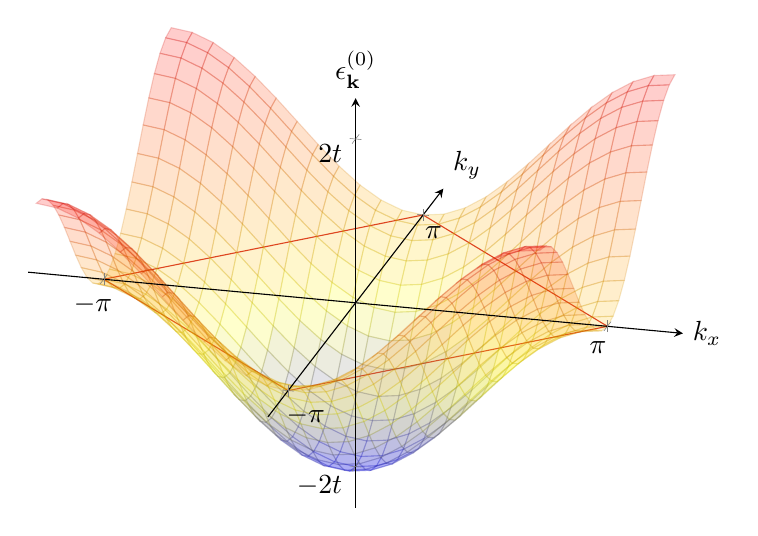
\begin{tikzpicture}
	\begin{axis}[
			axis on top,
			axis lines=center,
			xmin=-1.3, xmax=1.3,
			ymin=-1.3, ymax=1.3,
			zmin=-2.5, zmax=2.5,
			xtick={-1,1},
			ytick={-1,1},
			ztick={-2,2},
			xticklabels={$-\pi$,$\pi$},
			yticklabels={$-\pi$,$\pi$},
			zticklabels={$-2t$,$2t$},
			xlabel={$k_x$},
			ylabel={$k_y$},
			zlabel={$\epsilon_{\mathbf{k}}^{(0)}$},
			xlabel style={anchor=west},
			ylabel style={anchor=south west},
			zlabel style={anchor=south},
			width=\textwidth,
			view/az=15,
			view/el=30
		]
		\addplot3[
			domain=-1:0,
			color=tabred,
			dashed,
		]
		(
			{x},
			{-1-x},
			{0}
		);
		\addplot3[
			domain=0:1,
			color=tabred,
			dashed,
		]
		(
			{x},
			{-1+x},
			{0}
		);
		\addplot3[
			domain=-1:0,
			color=tabred,
			dashed,
		]
		(
			{x},
			{1+x},
			{0}
		);
		\addplot3[
			domain=0:1,
			color=tabred,
			dashed,
		]
		(
			{x},
			{1-x},
			{0}
		);
		
		\addplot3[
			domain=-1:1,
			samples=25,
			smooth,
			surf,
			opacity=0.2
		] { -cos(deg(pi*x))-cos(deg(pi*y)) };
		
		
	\end{axis}
\end{tikzpicture}
	\caption{Depiction of the Hubbard square lattice hopping band $\epsilon_{\mathbf{k}}^{(0)} = -2t[\cos(k_x) + \cos(k_y)]$. The red lines mark the zero-energy intersection.}
	\label{appfig:ferromagnetic-3d-band}
\end{figure}

{\color{tabred} Unclear: numerically, it turns out the paramagnetic phase ($m=0$) is preferred. Let $\Delta \equiv Um$ and ignore the constant contribution to energies $Un$: graphically, the $\uparrow$ band is shifted by $\Delta$, the $\downarrow$ band by $-\Delta$. At half-filling the Fermi energy remains fixed. For each quadrant (top view of the bands), the DoS is inversion-symmetric with respect to the anti-diagonal (red lines in Fig.~\ref{appfig:ferromagnetic-3d-band}), thus filling the bands bottom-up while performing the shifts should leave the total energy unchanged. Why is $m=0$ preferred?}

\section{Antiferromagnetic solution}

Consider now an AF mean-field solution. Let me change notation for a brief moment, indicating each site as
\[
	i \to \mathbf{r} = (x,y)
	\qquad
	x,y \in \mathbb{N}
\]
The mean-field AF solution at half-filling is the uniform-modulated magnetization
\[
	m_\mathbf{r} = (-1)^{x+y} m
	\qquad
	m \in [-1,1]
\]
and a mean-field Ansatz
\[
	\ev{\hat n_{\mathbf{r}\uparrow}} = n+m_\mathbf{r}
	\qquad
	\ev{\hat n_{\mathbf{r}\downarrow}} = n-m_\mathbf{r}
\]
With respect to the solution presented above, the only detail changing is the last term,
\[
	\hat H = -t \sum_{\langle \mathbf{r}\mathbf{r}' \rangle} \sum_\sigma \hat c_{\mathbf{r}\sigma}^\dagger \hat c_{\mathbf{r}'\sigma}
	+ nU \sum_\mathbf{r} \left[
		\hat n_{\mathbf{r}\uparrow} + \hat n_{\mathbf{r}\downarrow}
	\right] + mU \sum_\mathbf{r} (-1)^{x+y} \left[
		\hat n_{\mathbf{r}\uparrow} - \hat n_{\mathbf{r}\downarrow}
	\right]
\]
Fourier-transforming, the phase factor can be absorbed in the destruction operator inside of $\hat n_{\mathbf{r}\sigma}$:
\[
\begin{aligned}
	\sum_\mathbf{r} (-1)^{x+y} \hat n_{\mathbf{r}\sigma} &= \sum_\mathbf{r} (-1)^{x+y} \hat c_{\mathbf{r}\sigma}^\dagger \hat c_{\mathbf{r}\sigma} \\
	&= 
	\sum_\mathbf{r} e^{i \bm{\pi} \cdot \mathbf{r}}
	\frac{1}{N} \sum_{\mathbf{k} \in \mathrm{BZ}} e^{i \mathbf{k} \cdot \mathbf{r}} \hat c_{\mathbf{k}\sigma}^\dagger \frac{1}{N} \sum_{\mathbf{k}' \in \mathrm{BZ}} e^{-i \mathbf{k}' \cdot \mathbf{r}} \hat c_{\mathbf{k}'\sigma} \\
	&= \sum_{\mathbf{k} \in \mathrm{BZ}} \sum_{\mathbf{k}' \in \mathrm{BZ}} \hat c_{\mathbf{k}\sigma}^\dagger \hat c_{\mathbf{k}'\sigma} \frac{1}{N^2} \sum_\mathbf{r} e^{-i [\mathbf{k}' - (\mathbf{k} + \bm{\pi}) ] \cdot \mathbf{r}} \\
	&= \sum_{\mathbf{k} \in \mathrm{BZ}} \hat c_{\mathbf{k}\sigma}^\dagger \hat c_{\mathbf{k}+\bm{\pi}\sigma}
\end{aligned}
\]
where $\bm{\pi} = (\pi,\pi)$. It follows:
\[
mU \sum_\mathbf{r} (-1)^{x+y} \left[
		\hat n_{\mathbf{r}\uparrow} - \hat n_{\mathbf{r}\downarrow}
	\right] = \Delta \sum_{\mathbf{k} \in \mathrm{BZ}} \left[
		\hat c_{\mathbf{k}\uparrow}^\dagger \hat c_{\mathbf{k}+\bm{\pi}\uparrow} - \hat c_{\mathbf{k}\downarrow}^\dagger \hat c_{\mathbf{k}+\bm{\pi}\downarrow}
	\right]
	\qq{where}
	\Delta \equiv mU
\]
\begin{figure}
	\centering
	\subfloat[Alternative band.]{
		% It's easier to rotate coordinates and hide axis than
% define a tilted rectangular domain?

\begin{tikzpicture}
	\begin{axis}[
			axis on top,
			axis lines=none, % Support axis
			xmin=-1.3, xmax=1.3,
			ymin=-1.3, ymax=2.3,
			zmin=-2.5, zmax=2.5,
			view/az=65,
			view/el=30,
			width=0.7\textwidth
		]
		\addplot3[
			domain=-0.707:0.707,
			color=tabred,
		]
		(
			{x},
			{0.707},
			{0}
		);
		\addplot3[
			domain=-0.707:0.707,
			color=tabred,
		]
		(
			{x},
			{-0.707},
			{0}
		);
		\addplot3[
			domain y=-0.707:0.707,
			color=tabred,
		]
		(
			{0.707},
			{y},
			{0}
		);
		\addplot3[
			domain y=-0.707:0.707,
			color=tabred,
		]
		(
			{-0.707},
			{y},
			{0}
		);
		
		\draw[color=black, line width=0.2pt, -stealth]
			(0,0,0) -- (0.2,0.2,0) node[anchor=west, yshift=-0.2em]
				{\tiny $k_x$};
		\draw[color=black, line width=0.2pt, -stealth]
			(0,0,0) -- (-0.25,0.25,0) node[anchor=south, xshift=0.2em, yshift=-0.1em]
				{\tiny $k_y$};
		
		\node[color=tabred, anchor=south, yshift=0.2em]
			at (-0.707,0,0)
				{$\mathrm{MBZ}$};

		\draw[color=gray, -stealth]
			(0,0,0) -- (0,{sqrt(2)},0);

		\fill[color=tabred]
			(0,0,0) circle (1pt) node[anchor=east]
				{$\mathbf{0}$};
		
		\fill[color=tabblue]
			(0,{sqrt(2)},0) circle (1pt) node[anchor=west]
				{$\bm{\pi}$};
		
		\addplot3[
			domain=-0.707:0.707,
			y domain=-0.707:2.121,
			samples=25,
			smooth,
			surf,
			opacity=0.2,
			colormap name=tab
		] { -cos(deg(
				pi * (x-y)/sqrt(2)	% Rotated coordinates
			))-cos(deg(
				pi* (x+y)/sqrt(2)	% Rotated coordinates
			)) };
	\end{axis}
\end{tikzpicture}
		\label{appsubfig:alternative-ferromagnetic-3d-band}
	}
	\subfloat[Contour plot.]{
		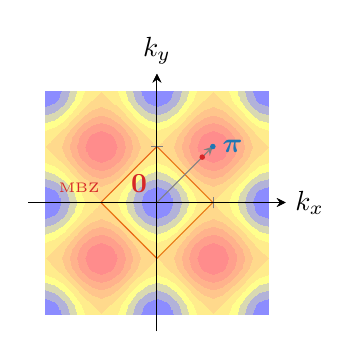
\begin{tikzpicture}
	\begin{axis}[
			axis x line=center,
			axis y line=center,
			axis z line=none,
			xmin=-2.3, xmax=2.3,
			ymin=-2.3, ymax=2.3,
			zmin=-2.5, zmax=2.5,
			xtick={1},
			ytick={1},
			xticklabel={$\pi$},
			yticklabel={$\pi$},
			xlabel={$k_x$},
			ylabel={$k_y$},
			xlabel style={anchor=west},
			ylabel style={anchor=south},
			view/az=0,
			view/el=90,
			width=0.4\textwidth,
			height=0.4\textwidth
		]
		\addplot3[
			domain=-1:0,
			color=tabred,
			dashed,
		]
		(
			{x},
			{-1-x},
			{0}
		);
		\addplot3[
			domain=0:1,
			color=tabred,
			dashed,
		]
		(
			{x},
			{-1+x},
			{0}
		);
		\addplot3[
			domain=-1:0,
			color=tabred,
			dashed,
		]
		(
			{x},
			{1+x},
			{0}
		);
		\addplot3[
			domain=0:1,
			color=tabred,
			dashed,
		]
		(
			{x},
			{1-x},
			{0}
		);
		
		\addplot3[
			domain=-2:2,
			samples=25,
			smooth,
			contour filled={number=10},
			fill opacity=0.45,
		] { -cos(deg(pi*x))-cos(deg(pi*y)) };
		
		\node[color=tabred, anchor=south east, xshift=0.3em]
			at (-1,0,0)
				{\tiny $\mathrm{MBZ}$};
		
		\draw[color=gray, -stealth]
			(0,0,0) -- (1,1,0);
		
		\fill[color=tabred]
			(0,0,0) circle (0pt) node[anchor=south east]
				{$\mathbf{0}$};
		
		\fill[color=tabblue]
			(1,1,0) circle (1pt) node[anchor=west]
				{$\bm{\pi}$};
		
	\end{axis}

	% Fine tuned
	\fill[color=tabred]
		(2.21,2.21) circle (1pt);
	
\end{tikzpicture}
		\label{appsubfig:ferromagnetic-contour}
	}
	\caption{Alternative depiction of the Hubbard square lattice hopping band previously reported in Fig.~\ref{appfig:ferromagnetic-3d-band}. The Magnetic Brillouin Zone ($\mathrm{MBZ}$) is delimited by the zero-energy contour and is indicated in figure. As it is evident, energy sign flips by taking a $(\pi,\pi)$ translation in $\mathbf{k}$ space.}
	\label{appfig:alternative-ferromagnetic-band}
\end{figure}

Consider the band of Fig.~\ref{appfig:ferromagnetic-3d-band} at half-filling. As does \citeauthor{fabrizio2022course} \cite{fabrizio2022course}, the area delimited externally by the solid lines at zero energy is denominated ``Magnetic Brillouin Zone'' ($\mathrm{MBZ}$). The periodicity of $\mathbf{k}$ space guarantees that the full $\mathrm{BZ}$ can be taken as well to be the one of Fig.~\ref{appsubfig:alternative-ferromagnetic-3d-band}. Then:
\[
\begin{aligned}
	\sum_{\mathbf{k} \in \mathrm{BZ}}
	\hat c_{\mathbf{k}\uparrow}^\dagger \hat c_{\mathbf{k}+\bm{\pi}\uparrow} &= \sum_{\mathbf{k} \in \mathrm{MBZ}}
	\left[
		\hat c_{\mathbf{k}\uparrow}^\dagger \hat c_{\mathbf{k}+\bm{\pi}\uparrow} + \hat c_{\mathbf{k}+\bm{\pi}\uparrow}^\dagger \hat c_{\mathbf{k}+2\bm{\pi}\uparrow}
	\right] \\
	&= \sum_{\mathbf{k} \in \mathrm{MBZ}}
	\left[
		\hat c_{\mathbf{k}\uparrow}^\dagger \hat c_{\mathbf{k}+\bm{\pi}\uparrow} + \hat c_{\mathbf{k}+\bm{\pi}\uparrow}^\dagger \hat c_{\mathbf{k}\uparrow}
	\right]
\end{aligned}
\]
and the same applies for spin $\downarrow$. Periodicity by shifts $2\bm{\pi}$ has been used. Now, define the Nambu spinors:
\[
	\hat \Psi_{\mathbf{k}\sigma} \equiv \begin{bmatrix}
		\hat c_{\mathbf{k}\sigma}^\dagger \\
		\hat c_{\mathbf{k}+\bm{\pi}\sigma}^\dagger 
	\end{bmatrix}
\]
and a spin-wise gap,
\[
	\Delta_\uparrow = \Delta
	\qquad
	\Delta_\downarrow = -\Delta
\]
At fixed filling, the $U$ term is a pure energy shift, thus will be neglected. The kinetic term transforms as
\[
\begin{aligned}
	-t \sum_{\langle ij \rangle} \sum_\sigma \hat c_{i\sigma}^\dagger \hat c_{j\sigma} &= \sum_{\mathbf{k} \in \mathrm{BZ}} \sum_\sigma \epsilon_\mathbf{k}^{(0)} \hat c_{\mathbf{k}\sigma}^\dagger \hat c_{\mathbf{k}\sigma} \\ 
	&= \sum_{\mathbf{k} \in \mathrm{MBZ}} \sum_\sigma \left[
		\epsilon_\mathbf{k}^{(0)} \hat c_{\mathbf{k}\sigma}^\dagger \hat c_{\mathbf{k}\sigma}
		+ \epsilon_{\mathbf{k}+\bm{\pi}}^{(0)} \hat c_{\mathbf{k}+\bm{\pi}\sigma}^\dagger \hat c_{\mathbf{k}+\bm{\pi}\sigma}
	\right] \\
	&= \sum_{\mathbf{k} \in \mathrm{MBZ}} \sum_\sigma \epsilon_{\mathbf{k}}^{(0)}  \left[
		\hat c_{\mathbf{k}\sigma}^\dagger \hat c_{\mathbf{k}\sigma}
		- \hat c_{\mathbf{k}+\bm{\pi}\sigma}^\dagger \hat c_{\mathbf{k}+\bm{\pi}\sigma}
	\right] \\ 
\end{aligned}
\]
In the second passage, the sum over the full $\mathrm{BZ}$ was written considering that the entirety of the zone is given by all the points in the $\mathrm{MBZ}$ plus their conjugates obtained by a $\bm{\pi}$ shift in the flipped band. As depicted in Fig.~\ref{appsubfig:alternative-ferromagnetic-3d-band}, kinetic energy is anti-periodic in $\mathbf{k}$ space by a vector $\bm{\pi}$. This anti-periodicity accounts for the minus sign arising in the third passage. The hamiltonian is then given by:
\[
	\hat H = \sum_{\mathbf{k} \in \mathrm{MBZ}} \sum_\sigma \hat \Psi_{\mathbf{k}\sigma}^\dagger \hat h_{\mathbf{k}\sigma} \hat \Psi_{\mathbf{k}\sigma}
	\qq{being}
	\hat h_{\mathbf{k}\sigma} \equiv \begin{bmatrix}
		\epsilon_\mathbf{k}^{(0)} & \Delta_\sigma \\
		\Delta_\sigma & - \epsilon_\mathbf{k}^{(0)}
	\end{bmatrix}
\]
Notice: the Nambu hamiltonian is a $2\times2$ matrix over the $\mathrm{MBZ}$ -- which is half the full $\mathrm{BZ}$, coherently with a solution which essentially bipartites the lattice giving back a double sized unit cell.

The system ground-state \todo
%\input{parts/appendices/mean-field-hubbard/hm-superconductivity} %TODO WRITE

\printbibliography \nocite{*}

\end{document}
